%%%%%%%%%%%%%%%%%%%%%%%%%%%%%%%%%%%%%%%%%
% kaobook
% LaTeX Template	
% Version 1.3 (December 9, 2021)
%
% This template originates from:
% https://www.LaTeXTemplates.com
%
% For the latest template development version and to make contributions:
% https://github.com/fmarotta/kaobook
%
% Authors:
% Federico Marotta (federicomarotta@mail.com)
% Based on the doctoral thesis of Ken Arroyo Ohori (https://3d.bk.tudelft.nl/ken/en)
% and on the Tufte-LaTeX class.
% Modified for LaTeX Templates by Vel (vel@latextemplates.com)
%
% License:
% CC0 1.0 Universal (see included MANIFEST.md file)
%
%%%%%%%%%%%%%%%%%%%%%%%%%%%%%%%%%%%%%%%%%

%----------------------------------------------------------------------------------------
%	PACKAGES AND OTHER DOCUMENT CONFIGURATIONS
%----------------------------------------------------------------------------------------

\documentclass[
	a4paper, % Page size
	fontsize=10pt, % Base font size
	twoside=false, % Use different layouts for even and odd pages (in particular, if twoside=true, the margin column will be always on the outside)
	%open=any, % If twoside=true, uncomment this to force new chapters to start on any page, not only on right (odd) pages
	%chapterentrydots=true, % Uncomment to output dots from the chapter name to the page number in the table of contents
	numbers=noenddot, % Comment to output dots after chapter numbers; the most common values for this option are: enddot, noenddot and auto (see the KOMAScript documentation for an in-depth explanation)
]{kaobook}

% Choose the language
\ifxetexorluatex
	\usepackage{polyglossia}
	\setmainlanguage{english}
\else
	\usepackage[english]{babel} % Load characters and hyphenation
\fi
\usepackage[english=british]{csquotes}	% English quotes


% Load packages for testing
\usepackage{blindtext}
%\usepackage{showframe} % Uncomment to show boxes around the text area, margin, header and footer
%\usepackage{showlabels} % Uncomment to output the content of \label commands to the document where they are used

% Load the bibliography package
\usepackage{kaobiblio}
\addbibresource{biblioFEM.bib} % Bibliography file

% Load mathematical packages for theorems and related environments
\usepackage[framed=true]{kaotheorems}

% Load the package for hyperreferences
\usepackage{kaorefs}

\usepackage{ marvosym }


%\usepackage{algorithmicsx} % http://ctan.org/pkg/algorithms
%\usepackage{algpseudocode} % http://ctan.org/pkg/algorithmicx

\graphicspath{{examples/documentation/images/}{images/}{../../../disciplinas2020/elemfin2020/2016/}} % Paths in which to look for images

\makeindex[columns=3, title=Alphabetical Index, intoc] % Make LaTeX produce the files required to compile the index

\makeglossaries % Make LaTeX produce the files required to compile the glossary
\newglossaryentry{computer}{
	name=computer,
	description={is a programmable machine that receives input, stores and manipulates data, and provides output in a useful format}
}

% Glossary entries (used in text with e.g. \acrfull{fpsLabel} or \acrshort{fpsLabel})
\newacronym[longplural={Frames per Second}]{fpsLabel}{FPS}{Frame per Second}
\newacronym[longplural={Tables of Contents}]{tocLabel}{TOC}{Table of Contents}

 % Include the glossary definitions

\makenomenclature % Make LaTeX produce the files required to compile the nomenclature

\DeclareMathOperator*{\argmin}{argmin}
\DeclareMathOperator*{\argmax}{argmax}
\newcommand*{\argminl}{\argmin\limits}
\newcommand*{\argmaxl}{\argmax\limits}


% Reset sidenote counter at chapters
%\counterwithin*{sidenote}{chapter}

%----------------------------------------------------------------------------------------

\begin{document}

%----------------------------------------------------------------------------------------
%	BOOK INFORMATION
%----------------------------------------------------------------------------------------

\titlehead{\texttt{ICMC-USP}}
\subject{Lecture Notes \\ \textbf{Curso de Difuss\~ao}}

\title[]{Automatic solution of PDEs with the Finite Element platform {\normalfont\texttt{FEniCSx}}}
\subtitle{A hands-on course}

\author[RFA \& IB]{Roberto F. Ausas \\ \& \\ Igor Almeida Baratta} %\thanks{A \LaTeX\ lover}}

\date{\today}

\publishers{Instituto de Ci\^encias Matem\'aticas e de Computa\c{c}\~ao\\ University of S\~ao Paulo}

%----------------------------------------------------------------------------------------

\frontmatter % Denotes the start of the pre-document content, uses roman numerals

%----------------------------------------------------------------------------------------
%	OPENING PAGE
%----------------------------------------------------------------------------------------

%\makeatletter
%\extratitle{
%	% In the title page, the title is vspaced by 9.5\baselineskip
%	\vspace*{9\baselineskip}
%	\vspace*{\parskip}
%	\begin{center}
%		% In the title page, \huge is set after the komafont for title
%		\usekomafont{title}\huge\@title
%	\end{center}
%}
%\makeatother

%----------------------------------------------------------------------------------------
%	COPYRIGHT PAGE
%----------------------------------------------------------------------------------------

\makeatletter
\uppertitleback{\@titlehead} % Header

\lowertitleback{
	\textbf{Disclaimer}\\
	You can edit this page to suit your needs. For instance, here we have a no copyright statement, a colophon and some other information. This page is based on the corresponding page of Ken Arroyo Ohori's thesis, with minimal changes.
	
	\medskip
	
	\textbf{No copyright}\\
	\cczero\ This book is released into the public domain using the CC0 code. To the extent possible under law, I waive all copyright and related or neighbouring rights to this work.
	
	To view a copy of the CC0 code, visit: \\\url{http://creativecommons.org/publicdomain/zero/1.0/}
	
	\medskip
	
	\textbf{Colophon} \\
	This document was typeset with the help of \href{https://sourceforge.net/projects/koma-script/}{\KOMAScript} and \href{https://www.latex-project.org/}{\LaTeX} using the \href{https://github.com/fmarotta/kaobook/}{kaobook} class.
	
	The source code of this book is available at:\\\url{https://github.com/fmarotta/kaobook}
	
	(You are welcome to contribute!)
	
	\medskip
	
	\textbf{Publisher} \\
	First printed in January 2022 by \@publishers
}
\makeatother

%----------------------------------------------------------------------------------------
%	DEDICATION
%----------------------------------------------------------------------------------------

%\dedication{
%        Life is like a box of chocolates. You never know what you're gonna get.
%	\flushright -- Forrest Gump
%}

%----------------------------------------------------------------------------------------
%	OUTPUT TITLE PAGE AND PREVIOUS
%----------------------------------------------------------------------------------------

% Note that \maketitle outputs the pages before here

\maketitle


\definecolor{codegreen}{rgb}{0,0.6,0}
\definecolor{codegray}{rgb}{0.5,0.5,0.5}
\definecolor{codepurple}{rgb}{0.58,0,0.82}
\definecolor{backcolour}{rgb}{0.95,0.95,0.92}
\definecolor{gray}{rgb}{0.6, 0.6,0.6} 

\lstdefinestyle{mystyle}{
    backgroundcolor=\color{backcolour},   
    commentstyle=\color{codegreen},
    keywordstyle=\color{magenta},
    numberstyle=\tiny\color{codegray},
    stringstyle=\color{codepurple},
    basicstyle=\ttfamily\small,
    breakatwhitespace=false,         
    breaklines=true,                 
    captionpos=b,                    
    keepspaces=true,                 
    numbers=none,                    
    numbersep=5pt,                  
    showspaces=false,                
    showstringspaces=false,
    showtabs=false,                  
    tabsize=2
}
 
\lstset{style=mystyle}

% Python environment
\lstnewenvironment{python}[1][]
{
\pythonstyle
\lstset{#1}
}
{}

% Python for external files
\newcommand\pythonexternal[2][]{{
\pythonstyle
\lstinputlisting[#1]{#2}}}

% Python for inline
\newcommand\pythoninline[1]{{\pythonstyle\lstinline!#1!}}


%----------------------------------------------------------------------------------------
%	PREFACE
%----------------------------------------------------------------------------------------

%----------------------------------------------------------------------------------------
%	TABLE OF CONTENTS & LIST OF FIGURES/TABLES
%----------------------------------------------------------------------------------------

\begingroup % Local scope for the following commands

% Define the style for the TOC, LOF, and LOT
%\setstretch{1} % Uncomment to modify line spacing in the ToC
%\hypersetup{linkcolor=blue} % Uncomment to set the colour of links in the ToC
\setlength{\textheight}{230\hscale} % Manually adjust the height of the ToC pages

% Turn on compatibility mode for the etoc package
\etocstandarddisplaystyle % "toc display" as if etoc was not loaded
\etocstandardlines % "toc lines" as if etoc was not loaded

\tableofcontents % Output the table of contents

%\listoffigures % Output the list of figures

% Comment both of the following lines to have the LOF and the LOT on different pages
\let\cleardoublepage\bigskip
\let\clearpage\bigskip

%\listoftables % Output the list of tables

\endgroup

%----------------------------------------------------------------------------------------
%	MAIN BODY
%----------------------------------------------------------------------------------------

\mainmatter % Denotes the start of the main document content, resets page numbering and uses arabic numbers
\setchapterstyle{kao} % Choose the default chapter heading style

\chapter*{Preface}
\addcontentsline{toc}{chapter}{Preface} % Add the preface to the table of contents as a chapter


The finite element method (FEM) is by now one of the most popular
methods for numerically solving Partial Differential Equations (PDEs) in
science, engineering and applied mathematics. There are a number of
good reasons for this:

\begin{itemize}
	\item[\Smiley] For \textbf{elliptic}
	and \textbf{parabolic} problems\sidenote[][-0.2cm]{\textbf{Elliptic problems}:
		Stationary diffusion,
		heat conduction, fully developed laminar flows in ducts,
		linear elasticity.\\
		\textbf{Parabolic problems}:
		Transient diffusion or heat conduction, chemical kinetics,
		fluid dynamics.},
	the FEM provides very accurate solutions;\\
	
	\item[\Smiley] It is \textbf{general}, not restricted to linear problems,
	or to isotropic problems, or to any subclass of mathematical
	problems; \\
	
	\item[\Smiley] It is \textbf{geometrically flexible}, complex domains
	are quite easily treated, not requiring adaptations of the
	method itself; \\
	
	\item[\Smiley] It is \textbf{easy to code}, and the coding is quite problem-independent.
	Boundary conditions are much easier to deal with than in other methods; \\
	
	\item[\Smiley] It is \textbf{robust}, because in most cases the mathematical problem
	has an underlying variational structure (energy minimization, for example). \\
	
\end{itemize}

\begin{marginfigure}[-4.0cm]
	\hrule
	\vspace{0.1cm}
	\flushleft \textbf{\scriptsize Solid mechanics}
	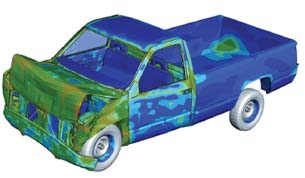
\includegraphics[width=0.8\textwidth]{truck}
	\vspace{0.1cm}       
	\hrule
	\vspace{0.1cm}
	\textbf{\scriptsize Heat transfer}
	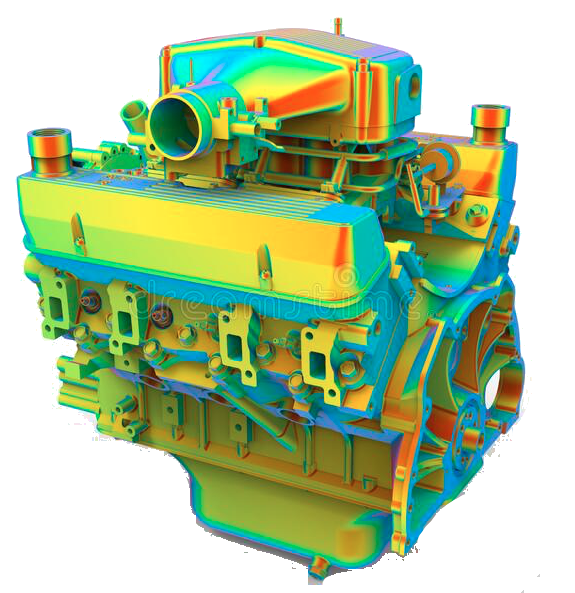
\includegraphics[width=0.7\textwidth]{engine2}
	\vspace{0.1cm}       
	\hrule
	\vspace{0.1cm}
	\textbf{\scriptsize Internal flows: Turbomachinery}
	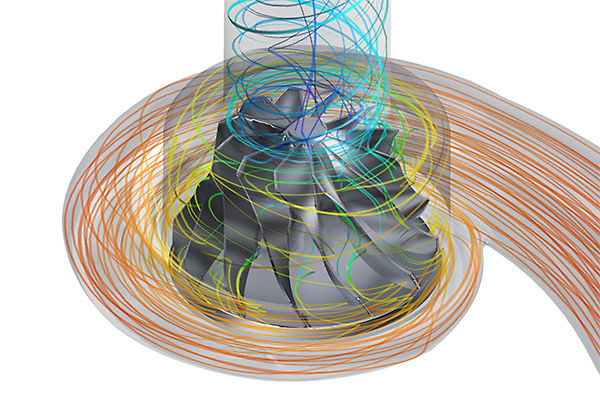
\includegraphics[width=0.8\textwidth]{turbine3}
	\vspace{0.1cm}
	\hrule
	\vspace{0.1cm}
	\textbf{\scriptsize Computational hemodynamics}
	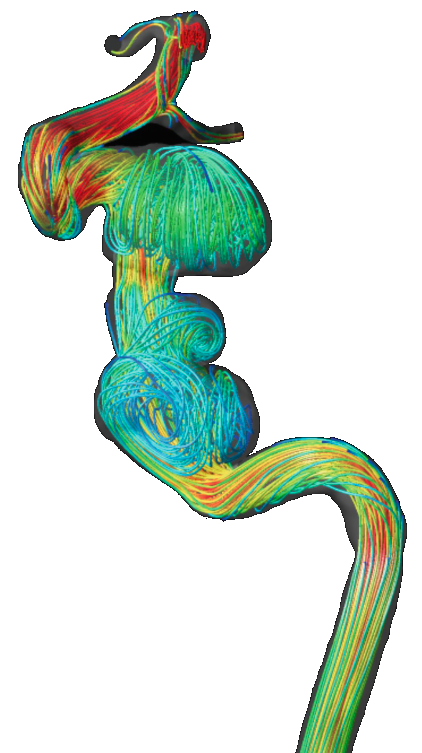
\includegraphics[width=0.5\textwidth,angle=90]{hemodyn2}
	\vspace{0.1cm}~\\
	\hrule
	\vspace{0.1cm}
	\textbf{\scriptsize External flows: Aerodynamics}
	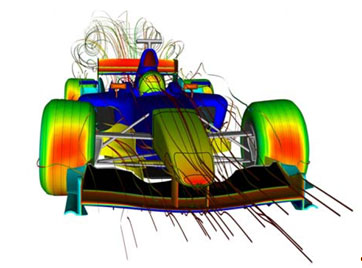
\includegraphics[width=0.8\textwidth]{f1formula}
	\vspace{0.1cm} 
	\hrule
	\caption[]{Examples solved by FEM.}
	\labfig{examples}
\end{marginfigure}

\section{What This Course Covers}
\labsec{does}

The main objective of this course is to introduce the student to the \href{https://fenicsproject.org/}{\texttt{FEniCSx}} open source platform for solving PDEs using the Finite Element method, through practical examples that arise in Solid and Fluid Mechanics.
The \texttt{FEniCS} project is a high-end open source platform that allows you to efficiently automate the resolution of partial differential equations (PDEs) by the finite element method (FEM). Through the use of a domain-specific language called UFL (Uniform Form Language) it is possible to write the variational formulation of complex problems governed by PDEs and their discretization by the FEM. Despite using a high-level language, the library allows solving problems efficiently with parallel computing, since it generates code in C that is compiled at runtime to perform the assembly of matrices and vectors that arise when applying the method. 

The course essentially consists of practical lectures on how to use the software to 
numerically solve some relevant 2nd order PDEs of interest in fluid and solid mechanics.  
Although the main focus of the course is practical (it will be a hands-on course), some mathematical and theoretical aspects will be recalled so as to provide the necessary context to understand the physical/mathematical problems considered and their numerical resolution by the finite element method. The target audience for the course is primarily graduate students, however, advanced undergrads in applied mathematics, physics or engineering courses are welcome to take the course. Students are expected to have minimal knowledge about PDEs and the physical models behind the problems to be solved. Some previous background about discretization methods for PDEs is also desirable.

The course will be divided into 5 lectures with the following topics to be covered: 

\begin{description}
	\item[Lecture |01|] Introduction:
	\begin{itemize}
		\item Examples of PDEs in fluid and solid mechanics
		\item Preliminary notions on the Finite Element Method
		\item The \texttt{FEniCSx} platform
		\item A first example: The heat conduction equation
	\end{itemize}
	
	\item[Lecture |02|] Classical problems:
	\begin{itemize}
		\item Transient heat conduction equation
		\item The elasticity problem
	\end{itemize}
	
	\item[Lecture |03|] Mixed problems:
	\begin{itemize}
		\item Coupled thermo-elasticity problem
		\item The Navier-Stokes equations
	\end{itemize}
	
	\item[Lecture |04|] Advanced topics: 
	
	\begin{itemize}
		\item Darcy's flow: $H(\mbox{div})$ formulations;
		\item Electromagnetism: The Helmholtz equation: 
	\end{itemize}
	
	\item[Lecture |05|] High Performance Computing with \texttt{FEniCSx}:
	
	\begin{itemize}
		\item Notions on parallel computing
		\item Scalability: Weak and Strong scaling
	\end{itemize}
	
\end{description}

\begin{flushright}
	\textit{RFA \& IAB} 
\end{flushright}

\index{preface}


\setchapterpreamble[u]{\margintoc}
\chapter{INTRODUCTION}
\labch{lec1}


\section{Motivating examples in solid and fluid mechanics}

We begin by recalling some prototypical examples of PDEs
we aim to solve by the finite element method.
We introduce things with a relatively informal language
and provide some physical interpretation of the different
quantities and processes involved.

\subsection{Poisson's equation} \index{Poisson's problem}

The simplest second order PDE we will consider in this course is
Poisson's equations that models several physical phenomena, such as,
heat conduction, mass transport by diffusion or even
fully developed flows in ducts as we will see later on in this
chapter. The problem reads: Given a region $\Omega \subset \mathbb{R}^d,~~d=1,2$ or $3$
with boundary $\partial{\Omega}$, find $u$ such as\sidenote{For $d = 2$, recall from Calculus,
the \emph{nabla} operator. In cartesian coordinates:
\begin{itemize}
\item The gradient of a scalar-valued function
$$
\nabla{f}  = \left (\dfrac{\partial{f}}{\partial{x}_1}, \dfrac{\partial{f}}{\partial{x}_2} \right)
$$
\item The divergence of a vector-valued function
$$
\nabla \cdot \mathbf{F} = \dfrac{\partial{F_1}}{\partial{x}_1} +  \dfrac{\partial{F_2}}{\partial{x}_2}
$$
\end{itemize}
}
\begin{equation}
\left \{
\begin{array}{rcll}
-\nabla \cdot \left ( \mu(\ex) \nabla{u}(\ex) \right) & = & f(\ex) & \ex \in \Omega \\
& & & \\
u(\ex) & = & g(\ex) & \ex \in \partial{\Omega}
\end{array}
\right.
\end{equation}

\begin{marginfigure}[3.0cm]
	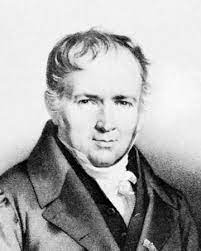
\includegraphics[width=0.65\textwidth]{Poisson}
	\caption[]{Sim\'eon Denis Poisson (France, 1781--1840).} 
	\labfig{domainfd}
\end{marginfigure}
%\begin{marginfigure}[3.5cm]
%       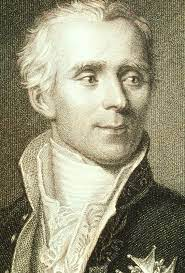
\includegraphics[width=0.65\textwidth]{Laplace}
%       \caption[]{Pierre-Simon Laplace (France, 1749--1827).} 
%\labfig{domainfd}
%\end{marginfigure}
where the source term $f:\Omega \rightarrow \mathbb{R}$ is a given function and
the boundary data $g:\partial{\Omega} \rightarrow \mathbb{R}$ is also a given
function. This problem falls into the cathegory of \textbf{elliptic} problems. 
The scalar field $u$ represents different physical quantities
depending on the problem. Notice that if $\mu$ is a constant, the left
hand side becomes the Laplace equation, i.e.,
\begin{equation}
\nabla \cdot \left ( \mu(\ex) \nabla{u}(\ex) \right) = \mu \, \nabla^2u(\ex)
\end{equation}
Of importance to us is a variant of this problem which includes flux boundary
conditions over all or in some part of $\partial{\Omega}$ (ommiting the
$\ex$ dependence for simplificity of notation)
\begin{equation}
\left \{
\begin{array}{rcll}
-\nabla \cdot \left ( \mu \nabla{u} \right) & = & f & \mbox{in}~~\Omega \\
& & & \\
u & = & g & \mbox{on}~~\Gamma_D \\
& & & \\
-\mu\,\nabla{u}\cdot \check{\mathbf{n}} & = & h & \mbox{on}~~\Gamma_N \\
\end{array}
\right.
\end{equation}
where $\partial{\Omega} = \Gamma_D \cup \Gamma_N$ and $\Gamma_D \cap \Gamma_N = \emptyset$
(see \reffig{domainGDGN}).
The so called mixed formulation introduces an additional field to represent
the flux of the quantity of interest
\begin{equation}
\left \{
\begin{array}{rcll}
\nabla \cdot \boldsymbol{\mathcal{J}} & = & f & \mbox{in}~~\Omega \\
& & & \\
\boldsymbol{\mathcal{J}} & = & -\mu\,\nabla{u} & \mbox{in}~~\Omega \\
& & & \\
u & = & g & \mbox{on}~~\Gamma_D \\
& & & \\
\boldsymbol{\mathcal{J}} \cdot \check{\mathbf{n}} & = & h & \mbox{on}~~\Gamma_N \\
\end{array}
\right.
\end{equation}
\begin{marginfigure}[-5.0cm]
	\includegraphics[]{Mixed_boundary_conditions}
	\caption[]{Domain $\Omega$ whose boundary is partitioned into a Dirichlet and a Neumann part.} 
	\labfig{domainGDGN}
\end{marginfigure}
Although both problems are equivalent in the exact setting we are
focused now, in the discrete setting things may differ a lot,
very different approaches being needed to deal with each formulation.
The equation defining the relation between $\boldsymbol{\mathcal{J}}$
and $u$ is what we call \textbf{constitutive law}.
Finally, it is instructive to interpret the different
quantities according to the physical problem being solved,
as summarized in table \reftab{physicaltable}.

\begin{table*}[ht]
\caption[]{Physical interpretation of quantities in Poisson's problem. Units in SI.}
\labtab{physicaltable}
\begin{tabular}{ c c c c c }
	\toprule
	Physical problem & $u$ & $f$ & $\boldsymbol{\mathcal{J}}$ & $\mu$  \\
	\midrule
	\multirow{3}{4em}{Heat conduction} & ~ & ~ & ~ & ~ \\
                                           & Temperature [{\footnotesize $^\circ K$}] & Heat source {\footnotesize [$\dfrac{\mbox{W}}{\mbox{m}^{3}}$]}  & Heat flux {\footnotesize [$\dfrac{\mbox{W}}{\mbox{m}^{2}}$]} & Conductivity {\footnotesize [$\dfrac{\mbox{W}}{\mbox{m} ^\circ \mbox{K}}$]} \\ 
                                           ~ & ~ & ~ & ~ & \\
	\multirow{3}{4em}{Mass diffusion} & ~ & ~ & ~& ~ \\
                                          & Mass {\footnotesize [$\dfrac{\mbox{mol}}{\mbox{m}^{3}}$]} & Mass source {\footnotesize [$\dfrac{\mbox{mol}}{\mbox{m}^{3}\mbox{s}}$]} & Mass flux {\footnotesize [$\dfrac{\mbox{mol}}{\mbox{m}^{2}\mbox{s}}$]}  & Diffusivity {\footnotesize [$\dfrac{\mbox{m}^2}{\mbox{s}}$]} \\ 
                                        ~ & ~ & ~ & ~ & \\
        \multirow{3}{4em}{Flow in ducts}  & ~ & ~ & ~& ~ \\
                                          & Velocity {\footnotesize [$\dfrac{\mbox{m}}{\mbox{s}}$]} & Pressure gradient {\footnotesize [$\dfrac{\mbox{N}}{\mbox{m}^3}$]} & Shear stress {\footnotesize [Pa]}  & Viscosity {\footnotesize [Pa $\cdot$ s]} \\ 
                                       ~  & ~ & ~ & ~ & \\
	\bottomrule
\end{tabular}
\end{table*}

\subsection{Transient heat conduction} \index{Transient heat equation}

The transient or unsteady version of the previous problems includes an additional term
involving the rate of change of the physical quantity of interest.
For the heat conduction problem the equation reads
\begin{equation}
\left \{
\begin{array}{rcll}
a(\mathbf{x},t)\,\dfrac{\partial{u}(\ex,t)}{\partial{t}} -\nabla \cdot \left ( \mu(\ex,t) \nabla{u}(\ex,t) \right) & = & f(\ex,t) & \ex \in \Omega,~~t \in [0,T] \\
& & & \\
u(\ex,t) & = & g(\ex,t) & \ex \in \partial{\Omega},~~t \in [0,T] \\
& & & \\
u(\ex,0) & = & u_0(\ex) & \ex \in \partial{\Omega}
\end{array}
\right.
\end{equation}
where now an initial condition for the scalar unknown (e.g. the temperature)
has been provided. This problem falls into the cathegory of \textbf{parabolic}
problems. The parameter $a$ in front of the time derivative
has different meanings depending on the problem at hand (see \reftab{physicaltabletran})
\begin{margintable}
\caption[]{Physical interpretation of the $a$ factor in front of $\partial_t{u}$ in the transient Poisson's problem. Units in SI.}
\labtab{physicaltabletran}
\begin{tabular}{ c c c }
	\toprule
	Problem & Factor $a$ & Description \\
	\midrule
	\multirow{3}{4em}{Heat conduction} & ~ & ~ \\
                                         ~ & $\rho \, c$ & ~ {\footnotesize [$\dfrac{\mbox{Kg}}{\mbox{m}^3}$~$\dfrac{\mbox{J}}{\mbox{Kg}\,^{\circ}\mbox{K}}$ ]}  \\ 
                                         ~ & ~ & ~  \\
	\multirow{3}{4em}{Mass diffusion} & ~ & ~ \\
                                        ~ & 1 &  {\footnotesize [-]}\\ 
                                        ~ & ~ & ~\\
        \multirow{3}{4em}{Flow in ducts}  & ~ & ~\\
                                        ~ & $\rho$ & {\footnotesize [$\dfrac{\mbox{Kg}}{\mbox{m}^3}$]}\\ 
                                        ~ & ~ & ~\\
	\bottomrule
\end{tabular}
\end{margintable}
The different forms of this problem, such as the one with a flux boundary condition
or the mixed formulation can be formulated in a similar way as in the stationary case.

\subsection{The equations of linear elasticity}

This is the prototypical example in solid mechanics in which we describe
the deformation of a solid domain. If we consider a
domain $\Omega \subset \mathbb{R}^d$ its shape is defined by
a map $\boldsymbol{\chi}: \Omega \rightarrow \mathbb{R}^d$, such that for any
$\mathbf{x} \in \Omega$ we write
\begin{equation}
\boldsymbol{\chi}(\mathbf{x},t) = \mathbf{x} + \mathbf{u}(\mathbf{x},t)
\end{equation}
where the vector field $\mathbf{u}: \Omega \rightarrow \mathbb{R}^{d}$
represents the displacement at the fixed location in space $\mathbf{x}$.
The PDE governing the problem follows from Newton's
dynamical equilibrium equations: 
\begin{equation}
\underbrace{\rho(\mathbf{x}) \dfrac{\partial^2\mathbf{u}(\mathbf{x},t)}{\partial{t}^2}}_{\mbox{mass}~\times~\mbox{acceleration}} -~ \underbrace{\nabla \cdot \boldsymbol{\sigma}(\mathbf{x},t) = \mathbf{f}(\mathbf{x},t)}_{\mbox{Forces}}
\end{equation}
where the second order time derivative in the left hand side corresponds
to the acceleration and $\mathbf{f}$ in the right hand side to the body forces (e.g., gravity),
$\boldsymbol{\sigma}(\mathbf{x},t)$ defines the stresses in the body at location $\mathbf{x}$,
which under the small deformation assumption is given by
the \textbf{constitutive law}
\begin{equation}
\boldsymbol{\sigma} =  \underbrace{\mu \left (\nabla{\mathbf{u}} + \nabla^{\intercal}{\mathbf{u}} \right)}_{2\mu\,\boldsymbol{\varepsilon}(\mathbf{u})} ~+~
\lambda (\nabla \cdot \mathbf{u}) \, \mathbf{I} 
\end{equation}
where $\lambda$ and $\mu$ are known material parameters and $\mathbf{I}$ is the identity matrix of $d\times d$\sidenote{For $d = 2$,
in cartesian coordinates
\begin{itemize}
\item The stress tensor is the matrix
\begin{equation}
\boldsymbol{\sigma} = \begin{bmatrix}\sigma_{11} & \sigma_{12} \\\sigma_{21} & \sigma_{22} \end{bmatrix}\nonumber
\end{equation}
\item The divergence of $\boldsymbol{\sigma}$ is the vector
\begin{equation}
\nabla \cdot \boldsymbol{\sigma} = \begin{bmatrix} \frac{\partial{\sigma_{11}}}{\partial{x}_1} + \frac{\partial{\sigma_{12}}}{\partial{x}_2} \\  \frac{\partial{\sigma_{21}}}{\partial{x}_1} + \frac{\partial{\sigma_{22}}}{\partial{x}_2} \end{bmatrix}\nonumber
\end{equation}
\item The gradient of the vector  field $\mathbf{u}$ is the matrix
\begin{equation}
\nabla\mathbf{u} = \begin{bmatrix} \frac{\partial{u_1}}{\partial{x}_1} & \frac{\partial{u_1}}{\partial{x}_2} \\
 \frac{\partial{u_2}}{\partial{x}_1} & \frac{\partial{u_2}}{\partial{x}_2} \end{bmatrix}\nonumber
\end{equation}
 \end{itemize}}.
In the stationary case this is an elliptic problem in which
the unknown field is a vector-valued function.
In order to have a well-posed problem the displacement
must be restricted in some part of the boundary (say, $\Gamma_{\mathbf{u}}$)
so as to eliminate rigid body motions (i.e., translations
and rotations). Also, a surface force distribution can be applied
on the rest of the boundary $\Gamma_{\boldsymbol{\mathcal{F}}} = \partial{\Omega} \setminus \Gamma_{\mathbf{u}}$.

\begin{equation}
\left \{
\begin{array}{rcll}
-\nabla \cdot \left ( 2\mu \boldsymbol{\varepsilon}(\mathbf{u}) + \lambda \, (\nabla\cdot\mathbf{u}) \, \mathbf{I}\right) & = & \mathbf{f} & \mbox{in}~\Omega \\
& & & \\
\mathbf{u} & = & \mathbf{u}_D & \mbox{on}~\Gamma_{\mathbf{u}} \\
& & & \\
(2 \mu \boldsymbol{\varepsilon}(\mathbf{u}) + \lambda \, (\nabla\cdot\mathbf{u})\,\mathbf{I})\cdot \check{\mathbf{n}} & = & \boldsymbol{\mathcal{F}} & \mbox{on}~\Gamma_{\boldsymbol{\mathcal{F}}}
\end{array}
\right.
\end{equation}
where $\mathbf{u}_D$ and $\boldsymbol{\mathcal{F}}$ are given functions.

\subsection{The incompressible Navier-Stokes problem}

A natural extension of the previous problem are
the Navier-Stokes equations. Now, we have two primary variables,
namely, the velocity field $\mathbf{u}(\mathbf{x},t)$ and
the pressure field $p(\mathbf{x},t)$. We consider
an Eulerian formulatio, so, $\mathbf{u}$ is
the velocity at fixed position $\mathbf{x}$ in space.
Also, we restrict ourselves to the particular case
of incompressible fields, i.e.,
\begin{equation}
\nabla \cdot \mathbf{u} = \frac{\partial{u_1}}{\partial{x_1}} + \frac{\partial{u_2}}{\partial{x_2}} + \frac{\partial{u_3}}{\partial{x_3}} = 0
\end{equation}
The stresses in the fluid are described by the Cauchy stress tensor \index{Cauchy stress tensor}
\begin{equation}
\boldsymbol{\sigma}(\mathbf{x},t) = -p(\mathbf{x},t) \mathbf{I} + \boldsymbol{\sigma}^*(\mathbf{x},t)
\end{equation}
which is the sum of a volumetric part 
\begin{equation}
-p(\mathbf{x},t) \mathbf{I} = 
\begin{bmatrix}
-p & 0 & 0 \\
0 & -p & 0 \\
0 & 0 & -p
\end{bmatrix}
\end{equation}
and a deviatoric part
\begin{equation}
\boldsymbol{\sigma}^*(\mathbf{x},t)= 2 \, \mu \boldsymbol{\varepsilon}(\mathbf{u}) =
\mu \left (\nabla{\mathbf{u}} + \nabla^{\intercal}{\mathbf{u}} \right)
%=
%\mu
%\begin{bmatrix}
%2\frac{\partial{u_1}}{\partial{x}_1} & \frac{\partial{u_1}}{\partial{x}_2} + \frac{\partial{u_2}}{\partial{x}_1} & \frac{\partial{u_1}}{\partial{x}_3} + \frac{\partial{u_3}}{\partial{x}_1} \\
% & 2\frac{\partial{u_2}}{\partial{x}_2} &  \\
% &  &  2\frac{\partial{u_3}}{\partial{x}_3}
%\end{bmatrix}
\end{equation}
\begin{marginfigure}[-3.0cm]
	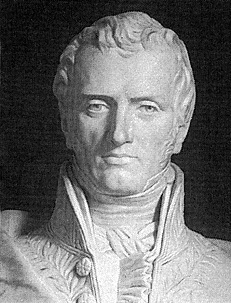
\includegraphics[width=0.65\textwidth]{Navier}
	\caption[]{Claude Louis Marie Henri Navier (France, 1785--1836).} 
	\labfig{navierphoto}
\end{marginfigure}
\begin{marginfigure}[3.0cm]
	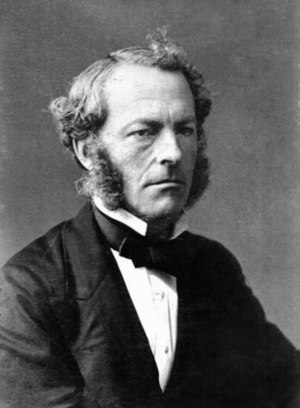
\includegraphics[width=0.65\textwidth]{Stokes}
	\caption[]{George Stokes (Ireland(1819)--England(1903)).} 
	\labfig{stokesphoto}
\end{marginfigure}
where $\mu$ is the viscosity of the fluid. Now, we write the momentum equation in the so called convective form
\begin{equation}
\rho\dfrac{D{\mathbf{u}}}{Dt} - \nabla \cdot\boldsymbol{\sigma} =  
\rho\left (\dfrac{\partial{\mathbf{u}}}{\partial{t}} +  \mathbf{u} \cdot \nabla \mathbf{u}\right ) 
- \nabla \cdot ( 2 \, \mu \boldsymbol{\varepsilon}(\mathbf{u})) + \nabla{p} = \mathbf{f}
\end{equation}
where the first (non-linear) term introduces the convective acceleration, the second term
the viscous effects and the third term the forces due to pressure gradients. As in the previous
case, in the left hand side we have the body forces (e.g., $\mathbf{f} = -\rho \, g  \check{\mathbf{e}}_3$).
Given an initial velocity field $\mathbf{u}_0$ that satisfies the incompressibility constraint,
the Navier-Stokes problem reads
\begin{equation}
\labeq{navierstokes}
\left\{
\begin{array}{ll}
\rho\left (\dfrac{\partial{\mathbf{u}}}{\partial{t}} +  \mathbf{u} \cdot \nabla \mathbf{u}\right )
- \nabla \cdot ( 2 \, \mu \boldsymbol{\varepsilon}(\mathbf{u})) + \nabla{p} = \mathbf{f} & \mbox{ in } \Omega \\
& \\
\nabla \cdot \mathbf{u} = 0  & \mbox{ in } \Omega \\
& \\
\mathbf{u} = \mathbf{u}_D & \mbox{ on } \Gamma_D \\
& \\
\left [-p\mathbf{I} + 2\,\mu\, \boldsymbol{\varepsilon}(\mathbf{u}) \right ] \cdot \check{\mathbf{n}} = \boldsymbol{\mathcal{F}} & \mbox{ on } \Gamma_N
\end{array}
\right.
\end{equation}
where $\mathbf{u}_D$ is a given function on $\Gamma_D$ and $\boldsymbol{\mathcal{F}}$ is
a given function on $\Gamma_N$.


\subsection{Electromagnetism: The Helmholtz's equation}

...

\section{A variational formulation}

The simplest example we can consider is the Poisson's problem
\begin{equation}
\left \{
\begin{array}{rcll}
-\nabla \cdot \left ( \mu \nabla{u} \right) & = & f & \mbox{in}~~\Omega \\
& & & \\
u & = & g_D & \mbox{on}~~\partial{\Omega}_D \\
& & & \\
-\mu\,\nabla{u}\cdot \check{\mathbf{n}} & = & g_N & \mbox{on}~~\partial{\Omega}_N \\
\end{array}
\right.
\end{equation}


We will proceed quite informally and letting some details for more advanced courses.
The idea first is to cast this problem into
variational form, which amounts to multiply by a sufficiently regular
\textbf{test} function $v$ that satifies the boundary condition, i.e.,
\begin{equation}
v(\mathbf{x}) = 0~~~\forall \mathbf{x} \in \partial{\Omega}_D \labeq{vzeroG}
\end{equation}
and integrate over $\Omega$, yielding
\begin{equation}
-\int_{\Omega}{\nabla\cdot \left ( \mu(\ex)\,\nabla{u}(\ex)\right ) \, {v}(\ex)}\,dx =
\int_{\Omega}{f(\ex)\,v(\ex)}\,dx \labeq{poissonbasicfv}
\end{equation}
From our Calculus course we know that (ommiting the $\mathbf{x}$ dependence to simplify notation)
\begin{equation}
\nabla \cdot \left(  \mu \nabla{u} \, v  \right) = \nabla \cdot \left(  \mu \nabla{u}  \right)\, v
+ \mu \nabla{u} \cdot \nabla{u} \nonumber
\end{equation}
We thus have
\begin{equation}
\int_{\Omega}{\mu\,\nabla{u}\cdot \nabla{v} }\,dx -\int_{\Omega}{\nabla \cdot \left(  (\mu \nabla{u}) \, v  \right)}\,dx  = 
\int_{\Omega}{f\,v}\,dx \labeq{poissonbasicfvfin}
\end{equation}
For the second term in the left hand side we apply Gauss theorem
\begin{equation}
\int_{\Omega}{\nabla \cdot \left(  (\mu \nabla{u}) \, v  \right)}\,dx  = \int_{\partial{\Omega}}{v\,(\mu \nabla{u})\cdot \check{\mathbf{n}}}\,ds
\end{equation}
which is identically zero on $\partial{\Omega}_D$ by \refeq{vzeroG}, yielding\sidenote{What we have done is also called integration by parts. Also notice that the boundary 
of $\Omega$ must have some regularity for the Gauss theorem to be applicable.}
\begin{equation}
\int_{\Omega}{\mu\,\nabla{u}\cdot \nabla{v} }\,dx = \int_{\Omega}{f\,v}\,dx - \int_{\partial{\Omega}_N}{g_N \, v}\,ds
\end{equation}
Let us agree that this should be valid for any $v$ belonging to some space of
functions $v: \Omega \rightarrow \mathbb{R}$ (say $V(\Omega)$) that satisfy
the homogeneous boundary conditions at $\partial{\Omega}_D$, for which the integrals
in the left and right hand sides at least don't blow up.
We may formally write what we call from now on the weak\sidenote{The problem is said to be in
	\textbf{weak} form because in this formulation we require less differentiability from
	$u$ in contrast to the PDEs in \textbf{strong} form for which we require $u$ to
	have at least continuous second order derivatives if we pretend the equation
	to be satisfied pointwise.} form of the problem
\begin{kaobox}[frametitle=Weak form of Poisson's problem]
	Find $u \in V(\Omega)$ such that
	\begin{equation}
	\left \{
	\begin{array}{ll}
	\underbrace{\int_{\Omega}{\mu(\ex)\,\nabla{u}(\ex)\cdot \nabla{v}(\ex)}\,dx}_{a(u,v)} =
	\underbrace{\int_{\Omega}{f(\ex)\,v(\ex)}\,dx - \int_{\partial{\Omega}_N}{g_N(\ex) \, v(\ex)}\,ds}_{\ell(v)} \labeq{poissonbasicfinal} & \\
	& \\
	\forall v \in V(\Omega). &
	\end{array}
	\right.
	\end{equation}
\end{kaobox}
What appears in the lhs is a bilinear form $a(\cdot,\cdot)$,
whereas in the rhs we have a linear form
$\ell(\cdot)$, two objects we will encounter frequently
in the course.

\section{Some important function spaces}

The main focus of this course is on the practical 
aspects of the FEM, however, it is useful to recall
a few definitions of function spaces that are 
very often found when solving PDEs by the finite element method.

The first example is the space $C^k(\Omega)$ defined as the set
of all real-valued functions that are continuous and have
its partial derivatives up to order $k$ also continuous
on $\Omega$, particular cases being
\begin{equation}
C^0(\Omega) = \{f: \Omega \rightarrow \mathbb{R} : f~\mbox{is continuous}~\forall x \in \Omega\} ~\dot{=}~ C(\Omega)
\end{equation}
and
\begin{equation}
C^{\infty}(\Omega) = \{f: \Omega \rightarrow \mathbb{R} : f~\mbox{has continuous derivatives of all orders}~\forall x \in \Omega\}
\end{equation}
Notice that $C^{\infty}(\Omega) \subset \dots \subset C^{k}(\Omega) \subset \dots \subset C^{0}(\Omega) = C(\Omega)$.

Another example that we will encounter frequently in this course is the space of
square integrable functions
\begin{equation}
L^2(\Omega) = \{f: \Omega \rightarrow \mathbb{R} : \int_{\Omega} f^2\,dx < +\infty\} \labeq{L2sp}
\end{equation}
and the space of square integrable functions whose derivatives are also
square integrable
\begin{equation}
H^1(\Omega) = \{f: \Omega \rightarrow \mathbb{R} : f \in L^2(\Omega)~~\mbox{and}~ \int_{\Omega}{(\nabla{f}\cdot\nabla{f})} \,dx < +\infty\} \labeq{H1sp}
\end{equation}
which is quite relevant to us \sidenote{In \refeq{H1sp}, since $\nabla{f}: \Omega \rightarrow \mathbb{R}^{d}$
(is a vector--valued function), the symbol ``$\cdot$'' stands for the inner (or usual ``dot'')
product of vectors, i.e.,  
$\nabla{f}(x) \cdot \nabla{f}(x) = \mathlarger{\sum}_{i=1}^{d}{(\nabla{f})_{i}(x)\,(\nabla{f})_{i}(x)} =
\mathlarger{\sum}_{i=1}^{d}{\frac{\partial{f}}{\partial{x_i}}(x) \, \frac{\partial{f}}{\partial{x_i}}(x)}$.}.

Both are Hilbert spaces, i.e.,
is a vector space equipped with an inner product, that
is also a complete metric space with respect to the norm induced by
the inner product.

The inner products are the $L^2(\Omega)$-inner product
\begin{equation}
(v,w)_{L^2(\Omega)} = \int_{\Omega}{v\,w}\,dx  \labeq{L2inner}
\end{equation}
and the $H^1(\Omega)$-inner product
\begin{equation}
(v,w)_{H^1(\Omega)} = \int_{\Omega}{\left (v\,w + \nabla{v} \cdot \nabla{w}\right )}\,dx \labeq{H1inner}
\end{equation}
which induce the norms

\begin{equation}
\|v\|_{L^2(\Omega)} = \left ( \int_{\Omega}{v^2}\,dx  \right )^{\frac12} \nonumber
\end{equation}
and the $H^1(\Omega)$-inner product
\begin{equation}
\|v\|_{H^1(\Omega)} = \left ( \int_{\Omega}{\left (v^2 + \nabla{v} \cdot \nabla{v}\right )}\,dx \right )^{\frac12}  \nonumber
\end{equation}

As a final example consider a subspace of the previous, made up of functions
that are equal to zero on the boundary $\Gamma = \partial{\Omega}$
\begin{equation}
H^1_0(\Omega) = \{f \in H^1(\Omega) : f|_{\Gamma} = 0 \}, \nonumber
\end{equation}
This one is also of particular interest to us, since it incorporates
a \textbf{boundary condition}\sidenote[][1.0cm]{
We use the notation $ f|_{\Gamma}$ to denote the restriction of a function
$f$ to the boundary $\Gamma$, i.e., the values of $f(x),~x \in \Gamma$.
To do this properly, we must introduce the \textbf{trace} operator
$\gamma: C(\bar{\Omega}) \rightarrow C(\Gamma),~~\gamma(f) = f|_{\Gamma}$.}. 
We will encounter such spaces frequently throughout. Moreover, 
we will need to construct finite dimensional subspaces of these spaces 
for the implementation of the FEM. 

\section{The Galerkin method}

A key ingredient of the finite elememt method, is the
Galerkin method (also referred to as Ritz-Galerkin) \index{Ritz-Galerkin method},
which takes as starting point the variational formulation. 
Let recall the abstract variational problem:~~
Find $u \in V$ such that
\begin{equation}
\left.
\begin{array}{rll}
a(u,v) & = & \ell(v)  ~~~\forall \, v \in V \\
\end{array}
\right. \nonumber
\end{equation}
of which we will see several examples in following lectures.
The idea behind the Galerkin method is simply to replace
the space $V$ by a finite dimensional space $V_h \subset V$.
The space $V_h$ can be spanned by a set of linearly
independent functions in $V$, $\{\phi_1,\phi_2,\dots,\phi_n\}$
\sidenote[][0.0cm]{Recall, the subindex $h$ is used
	to denote finite dimensional or discrete spaces. The $h$
	in the finite element method is related to the refinement
	of a partition of $\Omega$ (the mesh), such that $h \rightarrow 0$
	as $n \rightarrow \infty$.},
so, we write a discrete variational formulation:

\begin{kaobox}[backgroundcolor={blue!10!white}]
\textbf{VF}$_h$: Find $u_h \in V_h$ such that
\begin{equation}
\left.
\begin{array}{rll}
a(u_h,v_h) & = & \ell(v_h)  ~~~\forall \,v_h \in V_h \\
\end{array}
\right. \labeq{absVPdisc}
\end{equation}
\end{kaobox}

The interesting thing about the Galerkin method is that it provides
the \textbf{methodology} to compute $u_h$. If we choose a basis
$\{\psi_1,\psi_2,\dots,\psi_N\}$ of $V_h$ and define $u_h \in V_h$ by
\begin{equation}
u_h(\mathbf{x}) = \sum_{j=1}^{n}{\mathsf{U}_j \, \psi_j(\mathbf{x})} \labeq{ansatzuh}
\end{equation}
\begin{marginfigure}[0.0cm]
	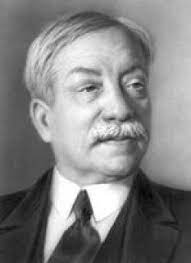
\includegraphics[width=0.65\textwidth]{Galerkin}
	\caption[]{Boris Galerkin (Russia, 1871-1945).}
	\labfig{galerkinphoto}
\end{marginfigure}
replace \refeq{ansatzuh} and take $w_h = \psi_i$ in \refeq{absVPdisc},
we obtain
\begin{equation}
a\left (\sum_{j=1}^{N}{\mathsf{U}_j\psi_j}, \psi_i\right) = \sum_{j=1}^{N}{\underbrace{a(\psi_j,\psi_i)}_{A_{ij}}\mathsf{U}_j} =
\underbrace{\ell(\psi_i)}_{b_i},~~~i=1,\dots,N
\end{equation}

\begin{kaobox}[backgroundcolor={blue!10!white}]
This clearly is a linear system of equations we can solve on a computer:
	
\begin{equation}
\mathbb{A} \, \boldsymbol{\mathsf{U}}
 = \boldsymbol{\mathsf{b}}
\end{equation}
where 
\begin{itemize}
\item $\boldsymbol{\mathsf{U}} = [\mathsf{U}_1, \mathsf{U}_2, \dots, \mathsf{U}_N]^{\intercal}$
is the vector of unknown degrees of freedom (dofs);
\item $\mathbb{A} \in \mathbb{R}^{N \times N}$ is the system matrix;
\item $\boldsymbol{\mathsf{b}} \in \mathbb{R}^{N}$ is the rhs vector,
\end{itemize}
which for our prototypical example of the heat diffusion problem, are defined by
\begin{equation}
A_{ij} = a(\psi_j,\psi_i) = \int_{\Omega}{\left ( \mu \, \nabla{\psi}_j \right )\cdot \nabla{\psi}_i }\,dv,
\end{equation}
and
\begin{equation}
b_i = \ell(\psi_i) = \int_{\Omega}{f \psi_i }\,dv.
\end{equation}

The size of the \textbf{Algebraic} problem to be solve clearly
depends on how big the dimension of the subspace $V_h$ is, and
for solving such system, \emph{Direct} or \emph{Iterative}
methods may be used.

\end{kaobox}

About matrix $\mathbb{A}$, in this particular case, we can say:
\begin{itemize}
	\item Since $a(v,w) = a(w,v)~\forall v,w \in V$ (i.e., $a(\cdot,\cdot)$ is symmetric),
	clearly $\mathbb{A}$ is also symmetric;\\
	\item if $a(w,w) > 0~\forall w \in V$ (then, $(\cdot,\cdot)$ is said to be strongly coercive\sidenote{Strong coercivity is also referred to as V-ellipticity. For
		the bilinear form at hand, it can be shown this property holds.}), taking
	any arbitrary nonzero $w_h = \sum_{j=1}^{N}{W_j \, \psi_j}$ and
	defining $\boldsymbol{\mathsf{W}} = [\mathsf{W}_1, \mathsf{W}_2, \dots, \mathsf{W}_N]^{\intercal}$, we get
	\begin{equation}
	a\left (\sum_{j=1}^{N}{\mathsf{W}_j\psi_j},\sum_{i=1}^{N}{\mathsf{W}_i\psi_i} \right) = \sum_{i=1}^{N}\sum_{j=1}^{N}{\mathsf{W}_i \, A_{ij} \, \mathsf{W}_j}
	= \boldsymbol{\mathsf{W}}^{\intercal} \mathbb{A} \boldsymbol{\mathsf{W}} > 0,~~\boldsymbol{\mathsf{W}} \ne \mathbf{0}
	\end{equation}
	thus, $\mathbb{A}$ is positive definite and therefore \textbf{invertible},
	so, we can safely solve the system and find the unique $\mathbf{U}$
	that defines $u_h$. \\
\end{itemize}

\section{Some classical Finite Element spaces}

The question that arises is how to construct a discrete space.
The typical choice is to construct piecewise polynomial spaces
associated to a \textbf{conforming partition} (a finite element mesh) 
of the computational domain,
i.e.,
\begin{equation}
V_h =  \{ w \in C^0(\bar{\Omega}),~\left. w \right |_K \in P_{k}(K)~~\forall K \in \mathcal{T}_h\} \nonumber
\end{equation}
where $P_{k}(K)$ is the space of polynomials of degree $k$ on $K$.
For instance, for $k = 1$ in 2D we have the classical \emph{hat} nodal functions
on 3-node triangular elements illustrated in \reffig{P1basis}.
\begin{equation*}
	P_1(K) = \{p: K \rightarrow \mathbb{R}, ~p = \alpha + \beta x + \gamma \, y \}   
\end{equation*}
\begin{marginfigure}[-5.0cm]
	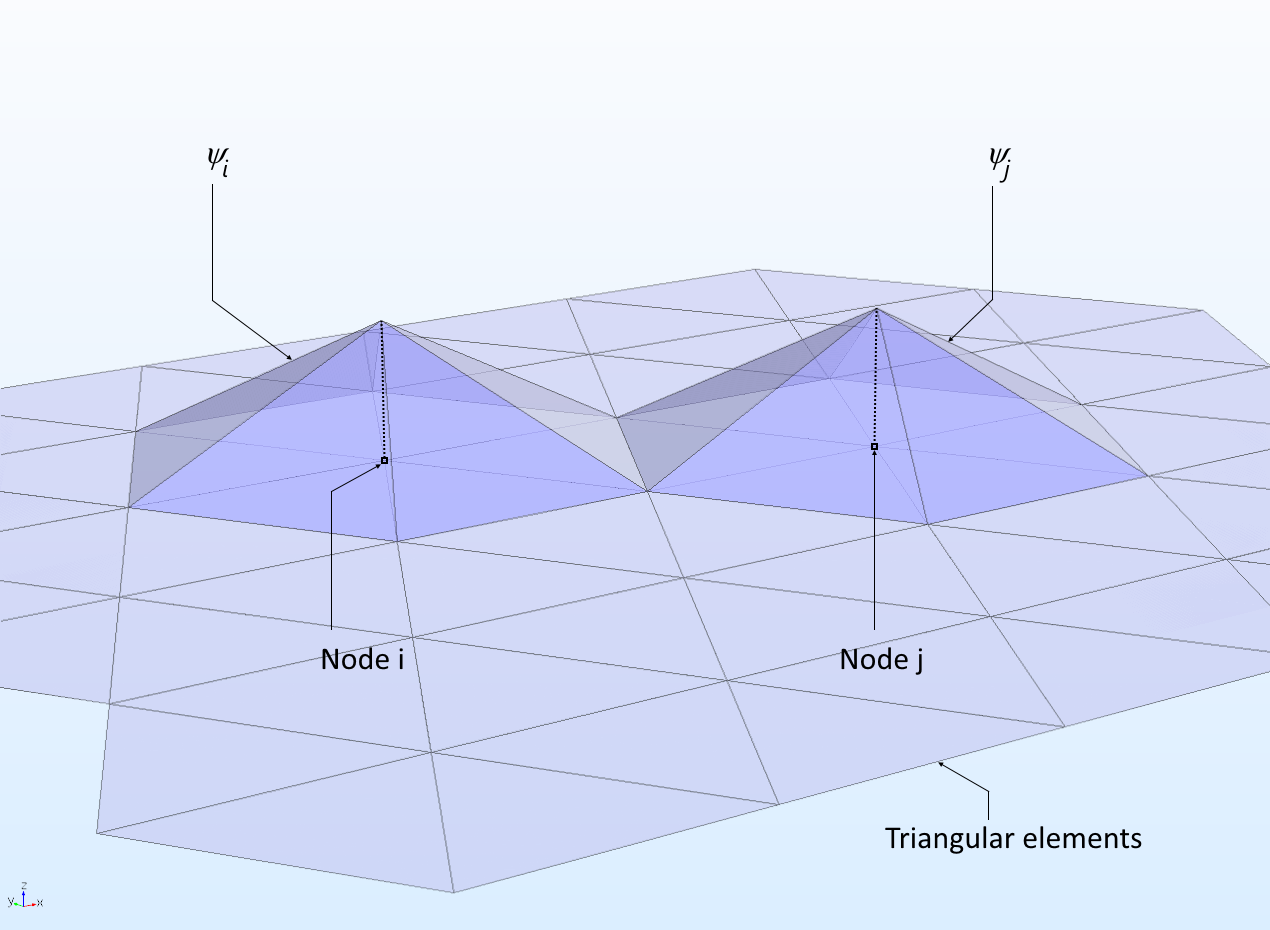
\includegraphics[width=1.25\textwidth]{base-functions-no-overlap.png}\\
	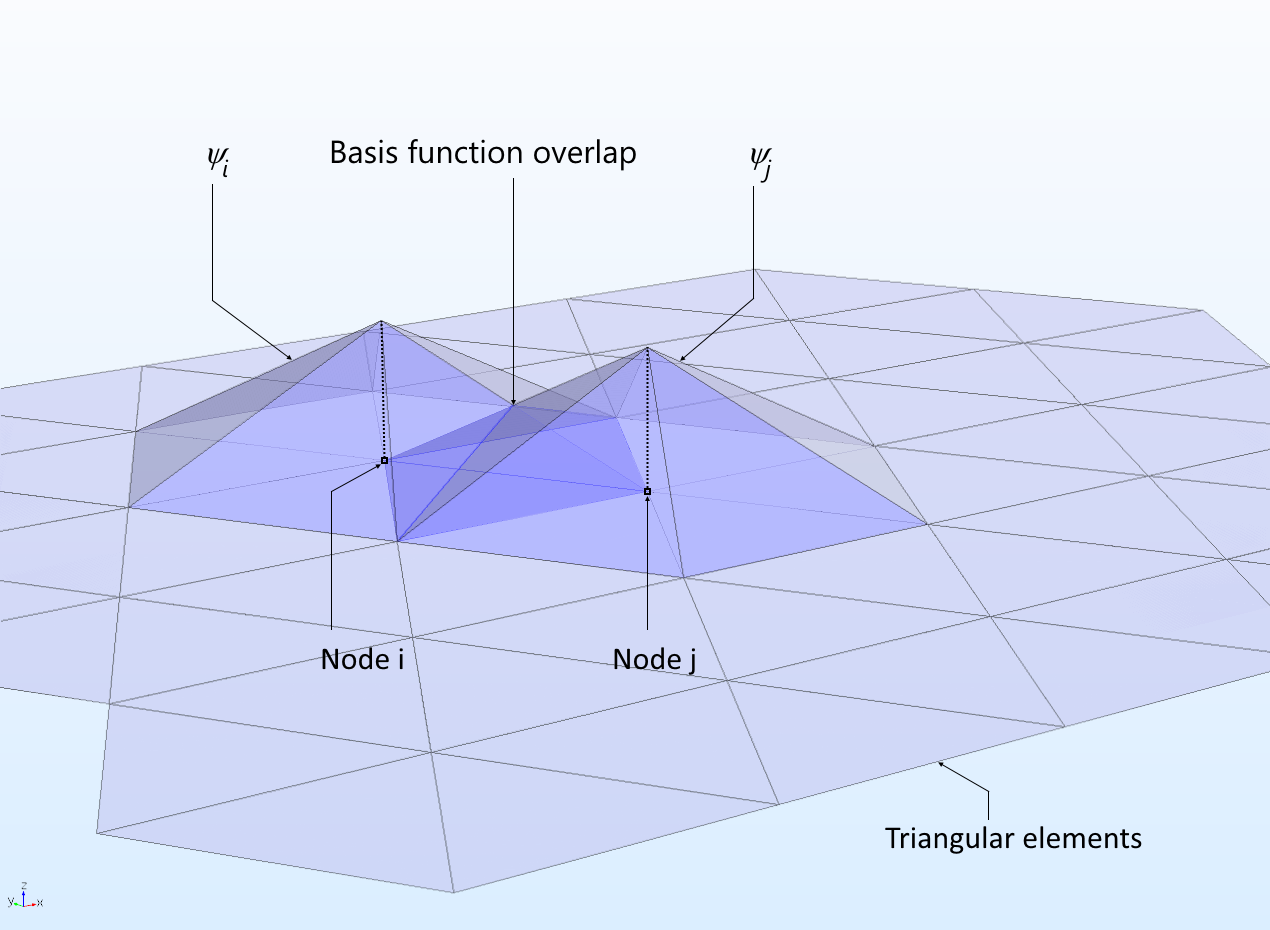
\includegraphics[width=1.25\textwidth]{base-functions-overlap.png}   
	\caption[]{Examples of $P_1$ basis functions associated to the nodes of a 2D triangular mesh.
		Source: \href{https://www.comsol.com/}{\texttt{https://https://www.comsol.com/}}.}
	\labfig{P1basis}
\end{marginfigure}

With these local functions, a global nodal base $\{\psi_1, \dots, \psi_n \}$, 
can be constructed, such that there is one function for each vertex (node)
of the mesh. Any piecewise linear function can be written as a
linear combination of such functions. They are constructed
such that the delta Kronecker property holds, i.e.,
$$
\psi_i(\mathbf{x}_j) = \delta_{ij}
$$
These are called \emph{Lagrangian} elements.
By looking at the basis functions illustrated in \reffig{P1basis}, we notice that they have
\textbf{compact support}, i.e, they are different than zero only in the cluster of elements
shared by a given node, thus leading to a sparse matrix $\mathbb{A}$.
Polynomials of higher order (quadratic, cubic, etc.) can be define similarly, just by introducing addition \textbf{degrees of freedom} (dofs).

An important concept for the construction of finite element spaces
as the ones just mentioned, is that of a finite element conforming mesh is, which 
we define here for completeness and ilustrate in \reffig{confvsnonconf}.
These are the type of meshes we will consider in this course.

\begin{definition}
	A partition $\mathcal{T}_h$ of a domain $\Omega$ is \textbf{ conforming} if $\bar{K}_i \cap \bar{K}_j$ is either
	\begin{itemize}
		\item empty, or,
		\item a vertex, or
		\item a complete edge.
		\item a complete face (in 3D)
	\end{itemize}
	otherwise the partition is said to be \textbf{ nonconforming}.
\end{definition}
\begin{marginfigure}[-10.0cm]
	\scalebox{1.3}{\input{images/meshes_f.pdf_t}}
	\caption[]{Conforming vs. nonconforming partitions of $\Omega$.}
	\labfig{confvsnonconf}
\end{marginfigure}


An interesting site to take a look at the different finite elements that have been invented 
so far (or, possibly, most of them) is the library \href{https://defelement.com/}{\texttt{DefElement}},
a project related to the \texttt{FEniCS} project.

\begin{figure}[ht!!]
\begin{center}
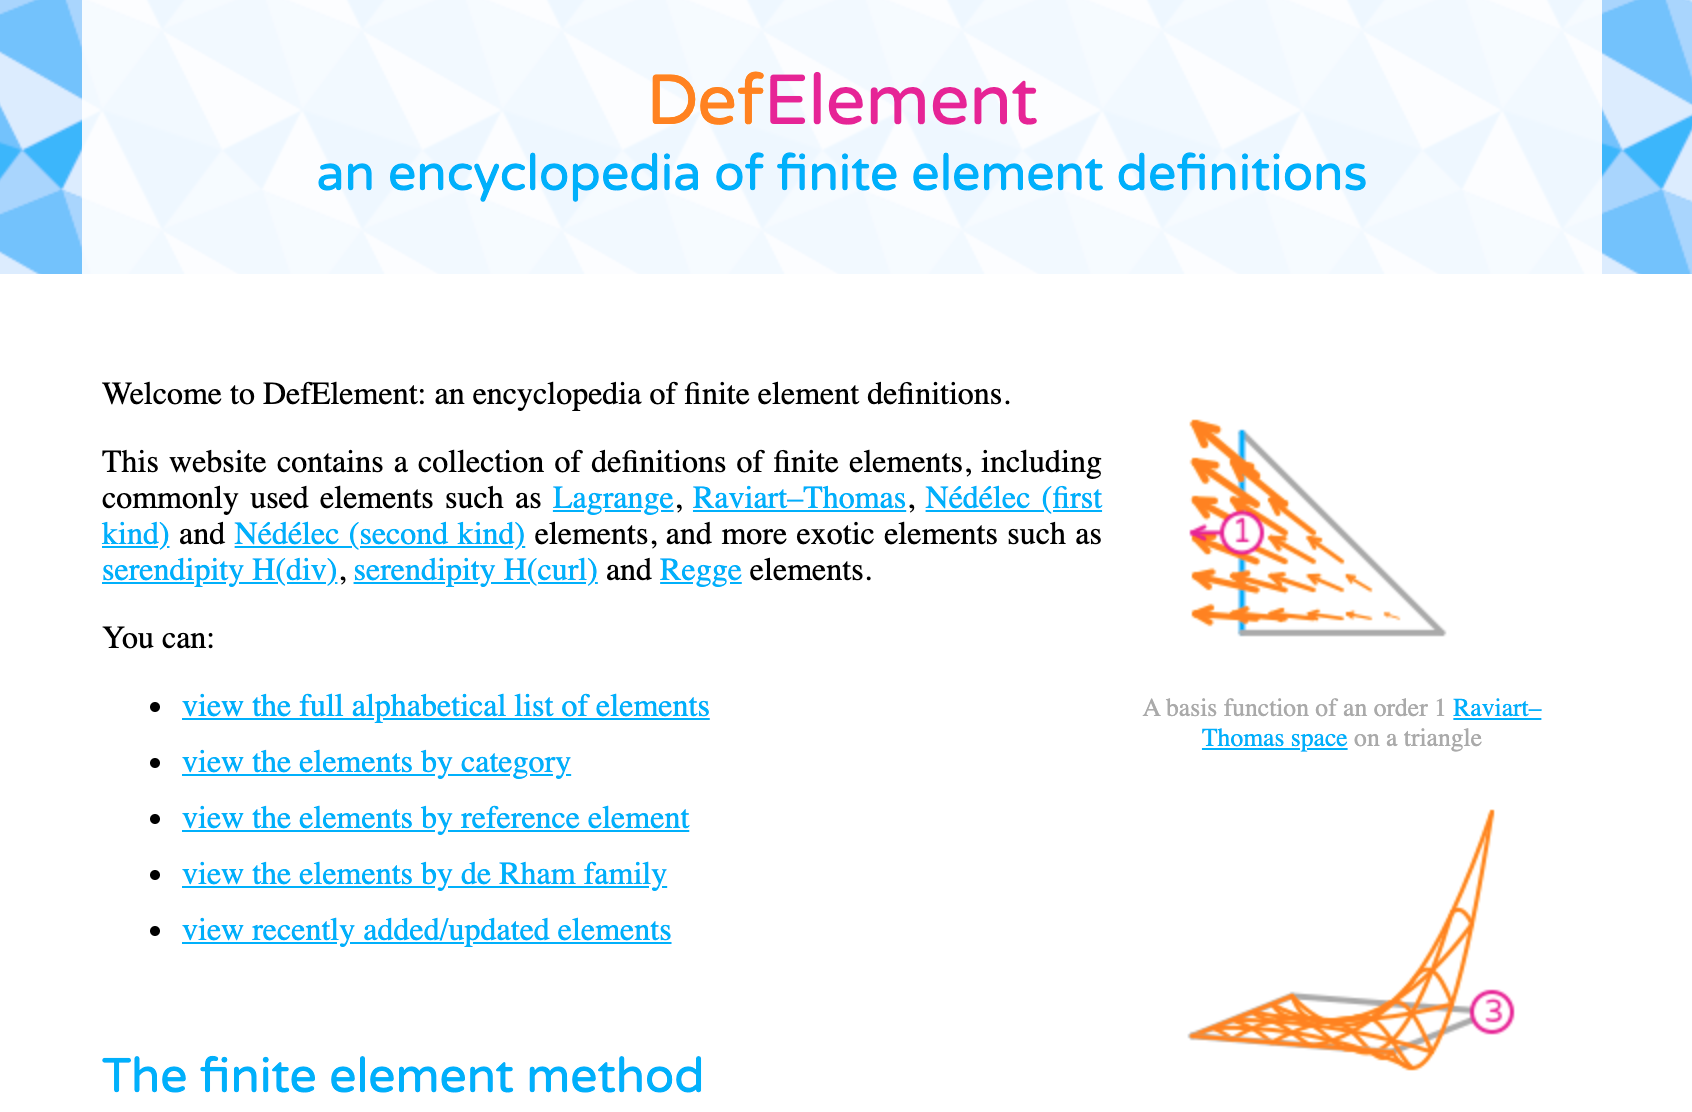
\includegraphics{defelement}
\end{center}
\end{figure}

We finally state the following theorem which is extremely important to the
FEM and justify the choice of piecewise polynomial spaces to approximate
the weak solution of PDEs:

\begin{theorem}
	Let $\Omega \subset \mathbb{R}^d$ be a bounded Lipschitz domain which can be
	partitioned into $N_e$ Lipschitz subdomains $K_j$ (i.e., $\overline{\Omega} = \bigcup_{j=1}^{N_e} \bar{K}_j$,	$K_i \cap K_j = \emptyset ~\forall i\ne j$. Let $v$ be a \textbf{ piecewise-polynomial} function on such a partition, then
	\begin{equation}
	v \in H^{1}(\Omega) \iff v \in C^0(\overline{\Omega}) \nonumber
	\end{equation}
	also
	\begin{equation}
	v \in H^{2}(\Omega) \iff v \in C^1(\overline{\Omega}) \nonumber
	\end{equation}
\end{theorem}



\section{The \texttt{FEniCSx} platform}

IGOR: MELHORAR ISTO

From the lectures, it will become quite clear that many of the computations
that are executed when using \texttt{FEniCSx} library, such as,
\textbf{construction of finite element spaces}, \textbf{assembly of finite element
	matrizes}, \textbf{numerical integration}, \textbf{imposition of boundary conditions},
\textbf{matrix solving}, and so on, 
remains totally hidden to the user. All these calculations being possible,
thanks to several components that form the \texttt{FEniCSx} platform. 
These are\sidenote{The
descriptions of the different components are just a brief summary taken from their corresponding
repository at \url{https://github.com/FEniCS}.}

\begin{enumerate}
	
	\item \href{https://github.com/FEniCS/dolfinx}{\texttt{UFL}}: \texttt{Python} library for writing problems
	in variational form. It
	provides the syntaxis to define linear and bilinear forms, finite elements spaces, such that the PDEs can 
	be written in weak form
	in a language that is close to the mathematical one;\\
	
	\item \href{https://github.com/FEniCS/dolfinx}{\texttt{DOLFINx}}: Dynamic Object Oriented Library for Fini
	te Element Computation.
	It provides the computational environment of FEniCSx in C++ and Python and serves, among other things,
	to interface to parallel linear algebra routines, such as \texttt{Petsc}; \\ 
	
	\item \href{https://github.com/FEniCS/ffcx}{\texttt{FFCx}}: FEniCS form compiler.  From a high-level descr
	iption of the form in the Unified Form Language (UFL), it generates efficient low-level C code that can be
	used to assemble the corresponding discrete operators. Also, the tutorial about \emph{Just-in-time-compilation} reveals interesting information (see \href{https://jorgensd.github.io/dolfinx-tutorial/chapter4/com
		piler_parameters.html}{\texttt{JIT}}); \\
	
	\item \href{https://github.com/FEniCS/basix}{\texttt{Basix}}: Is a finite element definition and tabulatio
	n runtime library.
	Basix allows users e.g. to evaluate finite element basis functions, access geometric and topological information about reference cells,
	interpolate into a finite element space, among other things;
	
\end{enumerate}

\section{1st Tutorial: \texttt{FEniCSx} implementation of Poisson's problem}

As already commented, we will adopt the \texttt{Colab notebook} environment
to present the different tutorials. For this first tutorial, 
we will present the \texttt{FEniCSx} implementation
of the prototypical elliptic second order problem, namely, the Poisson's 
equation, so, please, click in the link below in order to proceed

 \href{https://github.com/}{\texttt{|> Poisson's tutorial}}

\setchapterpreamble[u]{\margintoc}
\chapter{TWO CLASSICAL 2nd ORDER PROBLEMS}
\labch{lec2}

\section{Transient heat conduction}

\subsection{\texttt{FEniCSx} implementation}

\section{The elastostatic problem}

\subsection{\texttt{FEniCSx} implementation}


\iffalse

The plan for this lecture is:

\begin{itemize}
\item Present an implementation of the finite element discretization
of the Navier-Poisson elastostatic problem.
\item Create a non-trivial geometry and impose essential boundary conditions
on a vector field.
\item Visualize the solution using Paraview.
\item Perform some postprocessing of the solution.
\end{itemize}


\subsection{Mathematical formulation}

Let us recall the stationary linear elasticity problem with
Dirichlet and Neumann boundary conditions
\begin{equation}
\left \{
\begin{array}{rcll}
-\nabla \cdot \boldsymbol{\sigma} (\mathbf{u}) & = & \mathbf{f} & \mbox{in}~\Omega \\
& & & \\
\mathbf{u} & = & \mathbf{g} & \mbox{on}~\Gamma_{\mathbf{u}} \\
& & & \\
\boldsymbol{\sigma} \cdot \check{\mathbf{n}} & = & \boldsymbol{\mathcal{F}} & \mbox{on}~\Gamma_{\boldsymbol{\mathcal{F}}}
\end{array}
\right.
\end{equation}
where the stress tensor is
$$
\boldsymbol{\sigma} = 2\mu\, \boldsymbol{\varepsilon}({\mathbf{u}})+ \lambda \left ( \nabla\cdot\mathbf{u} \right )\, \mathbf{I}_{d \times d}
$$
where $d$ is the spatial dimension, $\mathbf{I}_{d \times d}$ is 
the identity tensor and the deformation tensor is defined by

$$
\boldsymbol{\varepsilon}({\mathbf{u}}) = \frac12 (\nabla{\mathbf{u}} + \nabla^{\intercal}{\mathbf{u}})
$$

Introducing the space of kinematically admissible motions

$$
V_{\mathbf{g}} = \{\mathbf{v} \in \left [ H^1(\Omega) \right ]^d,~\mathbf{v} = \mathbf{g}~\mbox{on}~\Gamma_D\}
$$

and applying the principle of virtual work, the variational formulation is obtained: 

\begin{kaobox}[frametitle=Weak form of the Elastostatic problem]
Find $\mathbf{u} \in V_{\mathbf{g}}$ such that

\begin{eqnarray}
\underbrace{\int_{\Omega}{\left [2\,\mu \boldsymbol{\varepsilon}(\mathbf{u}) : \boldsymbol{\varepsilon}(\mathbf{v})
		+ \lambda\, (\nabla \cdot \mathbf{u})\,(\nabla \cdot \mathbf{v}) \right ]\,dx}}_{a(\mathbf{u},\mathbf{v})} =
\underbrace{\int_{\Omega}{\mathbf{f}\cdot \mathbf{v}}\,dx +
	\int_{\Gamma_{\boldsymbol{\mathcal{F}}}}{\boldsymbol{\mathcal{F}} \cdot \mathbf{v}}\,ds}_{\ell(\mathbf{v})}\nonumber
\end{eqnarray}
$\forall \mathbf{v} \in V_{\mathbf{0}}$.
\end{kaobox}

The same could be obtained by multiplying the PDE by a sufficiently regular test
function $\mathbf{v}$ and integrating by parts, very much in the same way we 
proceeded with Poisson's problem.
It is very important to realize that functions $\mathbf{v} \in V_{\mathbf{0}}$ 
satisfy homegeneous boundary conditions on $\Gamma_D$.
Finally, the discrete version of this problem follows from applying 
the Galerkin method: 

\begin{kaobox}[backgroundcolor={blue!10!white}]
Find $\mathbf{u}_h \in V_{h\mathbf{g}} \subset V_{\mathbf{g}}(\Omega)$ such that

\begin{equation}
a(\mathbf{u}_h,\mathbf{v}_h) = \ell(\mathbf{v}_h) \nonumber
\end{equation}
$ \forall \mathbf{v}_h \in V_{h\mathbf{0}}$.

\end{kaobox}

We must create the discrete function space associated to the mesh $\mathcal{T}_h$. As in previous examples, a natural choice is a space of continuous vector functions, whose components 
are elementwise polynomials of degree $k$ (tipically, $k=1$ or $2$.)

$$
V(\mathcal{T}_h) = V_h = \{\mathbf{v} \in [H^1(\Omega)]^d,~\mathbf{v}|_E \in [P_k(E)]^d \, \forall E \in \mathcal{T}_h\}
$$

\subsection{Computational setting}

\begin{marginfigure}[-2.0cm]
\includegraphics[width=0.4\textwidth]{corpo_prova2d.png}
\caption[]{Computational domain to solve the elastostatic problem in 2D.
	The total height is $2.4$ units, the width and height of the bottom and top parts is $0.4$
	and the radius of the central arc (the neck) is $1.2$.}
\labfig{corpo2d}
\end{marginfigure}
In this tutorial we consider a more complex geometry which is ilustrated in 
\reffig{corpo2d}. This geometry is built using the \texttt{gmsh} library.
Notice how the mesh is refined locally in the thinner part of the domain.
On this geometry we will consider the following boundary conditions.
\begin{eqnarray}
\mathbf{u} & = & (0,0)^{\intercal} ~~\mbox{in}~~\Gamma_{\mbox{bottom}} \nonumber \\
& & \nonumber \\
u_x & = & 0~~\mbox{in}~~\Gamma_{\mbox{left}}\nonumber
\end{eqnarray}
These conditions ensure that \textbf{rigid body} motions, namely, \textbf{rotations and translations} are totally restricted. Usually, setting the boundary conditions is the step that takes more work. We must identify those degrees of freedom (the $\mathsf{U}_i$s) that correspond to points
located on the boundary and set accordingly by modifying the linear system of equations. 

As for the natural bounday conditions, on the top wall we will apply 
the following surface force distribution

$$
\boldsymbol{\mathcal{F}} = (0,-0.1)^{\intercal}
$$
so as to impose a compressive load. The rest of the boundary is traction free and the body forces are considered to be negligible, i.e.,

$$
\boldsymbol{\mathcal{F}} = (0,0)^{\intercal},~~~\mathbf{f} = (0,0)^{\intercal}
$$

\section{Homework 2}

\subsection{Von Mises stresses}

Given the deviatoric stresses 
$$
\boldsymbol{s} = \boldsymbol{\sigma}(\mathbf{u}_h) - \frac{\mbox{tr}(\boldsymbol{\sigma}(\mathbf{u}_h))}{d}\boldsymbol{I}_{d\times d}
$$

Compute the \textbf{scalar} quantity known as the Von Mises stresses
defined as the second invariant of the deviatoric stresses:

$$
\sigma_V = \sqrt{\frac32\boldsymbol{s}:\boldsymbol{s}}
$$

Implement in \texttt{dolfinx}. For visualization of results, interpolate $\sigma_V$ onto a space of elementwise constant functions (a \texttt{DG} space of order 0) as we have done before

$$
Q_h = \{v \in L^2(\Omega),~v|_E \in P_0(E) \, \forall E \in \mathcal{T}_h\}
$$

Follow the next guidelines:
\vspace{-0.5cm}
\begin{center}
	\begin{minipage}{1.05\textwidth}
		\lstinputlisting[language=Python]{vonmises.py}
	\end{minipage}
\end{center}


Notice the use of the \texttt{interpolate} method to assign to each 
element the corresponding value of $\sigma_V$.

\subsection{Optional: 3D problem}
\begin{marginfigure}[-3.0cm]
	\includegraphics[width=1.2\textwidth]{corpo_prova3d.png}
	\caption[]{Computational domain to solve the elastostatic problem in 3D.}
	\labfig{corpo3d}
\end{marginfigure}
Consider the 3D version of the previous problem which is shown
in \reffig{corpo3d}
This mesh can be created with the function \texttt{GenerateMesh3D()} available
at the end of the \texttt{notebook}. Implement the necessary changes to solve
the problem with the following boundary conditions
\begin{eqnarray}
\mathbf{u} & = & (0,0,0)^{\intercal} ~~\mbox{in}~~\Gamma_{\mbox{bottom}} \nonumber \\
& & \nonumber \\
\mathbf{u} & = & (0,0,-0.1)^{\intercal} ~~\mbox{in}~~\Gamma_{\mbox{top}} \nonumber
\end{eqnarray}
whereas the rest of the boundary remains traction free 
$$
\boldsymbol{\mathcal{F}} = (0,0)^{\intercal}
$$
\fi

%-----------------------------------------------
\setchapterpreamble[u]{\margintoc}
\chapter{MIXED PROBLEMS}
\labch{lec3}

\section{Thermoelastic problem}

\subsection{\texttt{FEniCSx} implementation}

\section{The incompressible Navier-Stokes equations}

\subsection{\texttt{FEniCSx} implementation}

%-----------------------------------------------
\setchapterpreamble[u]{\margintoc}
\chapter{ADVANCED TOPICS}
\labch{lec4}

\section{Darcy's flow}

\subsection{\texttt{FEniCSx} implementation}

\section{The Helmholtz's equation}

\subsection{\texttt{FEniCSx} implementation}

%-----------------------------------------------
\setchapterpreamble[u]{\margintoc}
\chapter{HIGH PERFORMANCE COMPUTING WITH \texttt{FEniCSx}}
\labch{lec5}


\section{Parallel computing in \texttt{FEniCSx}}

\section{Weak and strong scaling}

\subsection{\texttt{FEniCSx} implementation}


\iffalse

Prior to jumping into our first Miniproject/Assignment, let solve a few exercices that will
help us to get used with the previous problems:

\begin{kaobox}[frametitle=Exercices]

\begin{itemize}
\item Check the units of quantities in \reftab{physicaltable}. \\

\item Consider the Poisson's equation with $f = -6$ and $\mu = 1$
in the domain $\Omega = [0,1]^2$. Verify that 
\begin{equation}
u(x_1,x_2) = 1 + x_1^2 + 2\,x_2^2
\end{equation}
is a solution. Which boundary conditions this solution satisfies?\\

\item In the 2D case, consider a scalar function $\psi$ such that
\begin{equation}
u_1 = -\dfrac{\partial{\psi}}{\partial{x_2}},~~~u_2 = \dfrac{\partial{\psi}}{\partial{x_1}}
\end{equation}
($\psi$ is called the stream function). Show that $\nabla \cdot {\mathbf{u}} = 0$.\\

\item In the previous problem, compute the stress tensor $\boldsymbol{\sigma}$.\\


\item In the Navier-Stokes problem in 3D, write \emph{in extensum} the 3 momentum equations
corresponding to each component.\\

\item Consider the following \textbf{manufactured} solution in 2D for
the Navier-Stokes equations:
\begin{eqnarray}
\mathbf{u}(x_1,x_2,t) & = & \left [ \sin(x_1)\sin(x_2 + t), ~\cos(x_1)\cos(x_2 + t)\right]^{\intercal},\nonumber \\
p(x_1,x_2,t) & = & \cos(x_1) \sin(x_2 + t),\nonumber
\end{eqnarray}

Compute to which body force $\mathbf{f}$ and boundary conditions it corresponds.\\

\item Write the nondimensional form of the Navier-Stokes equations in terms
of nondimendional variables $\hat{\mathbf{u}}$, $\hat{\mathbf{x}}$, $\hat{p}$,
$\hat{t}$, $\hat{\mathbf{f}}$, the parameter and
Re$=\dfrac{\rho U L}{\mu}$ (a.k.a. the Reynolds number).

\end{itemize}

\end{kaobox}

\index{Fully developed flow}
\section{{\color{gray!50!blue} Assignment 1: Poisson's problem for fully developed flow}}

\begin{marginfigure}[-6.0cm]
\scalebox{0.8}{\input{images/pipes.pdf_t}}
       %\includegraphics[width=0.65\textwidth]{pipe_square.jpg}
       %\includegraphics[width=0.65\textwidth]{pipe_circular.jpg}
       \caption[]{Domain for the fully developed flow.} 
\labfig{domainfd}
\end{marginfigure}

\begin{kaobox}
Fully developed flow in ducts is a particular case of flow governed by the
Navier-Stokes equations, which corresponds to the following situation
(see \reffig{domainfd}):
\begin{itemize}
\item Incompressible flow along a long cylinder of 
cross section $\Omega\,\subset\,\mathbb{R}^2$. The flow
domain is $\mathcal{B}=\Omega\times (0,L)$.\\
\item The flow is driven by a uniform pressure gradient
\begin{equation}
\mathcal{G}(t)=\frac{p(L,t)-p(0)}{L}
\end{equation}
The pressure field is thus linear as a function of $x_3$.
Also, notice that when $\mathcal{G}(t)>0$ we expect $u_3<0$ and
viceversa. 
\\
\item If $L$ is sufficiently large, the entry and exit effects
can be neglected and all cross sections are essentially identical,
except for the pressure.\\

%\item Let $\omega$ be an arbitrary region in $\Omega$ and let $V$ be the
%corresponding cylinder, i.e.,
%\begin{equation}
%V=\omega\times (0,L)~.
%\end{equation}
%We denote also $\omega_z = \omega \times  \{z\}$ (the cross section at $x_3=z$) and 
%$\mathcal{S}=\partial \omega\times (0,L)$ (the lateral surface) so that
%\begin{equation}
%\partial V = \omega_0\,\cup\,\mathcal{S}\,\cup\,\omega_L~.
%\end{equation}

\item We consider as solution, velocity fields of the form:
\begin{equation}
\mathbf{u} = [0, 0, u(x_1,x_2,t)]^{\intercal}
\end{equation}

\item For any differentiable $u$, the proposed velocity is divergence free, i.e.,
\begin{equation}
\frac{\partial{u_1}}{\partial{x_1}} + \frac{\partial{u_2}}{\partial{x_2}} + \frac{\partial{u_3}}{\partial{x_3}}
=  \frac{\partial{u}}{\partial{x_3}} = 0
\end{equation}

\item Decomposing the stress tensor in pressure and non-pressure
components, we have
\begin{equation}
\boldsymbol{\sigma}(x_1,x_2,x_3,t)=-p(x_3,t)\,\mathbf{I}\,+\,\boldsymbol{\sigma}^*(x_1,x_2,t)~.
\label{eqstress3}
\end{equation}
where, if the fluid is Newtonian \index{Newtonian fluid}, 
\begin{equation}
\boldsymbol{\sigma}^*=\mu\,\left (
\begin{array}{ccc}
0 & 0 & u_{,1} \\ 0 & 0 & u_{,2} \\ u_{,1} & u_{,2} & 0
\end{array} \right )
\qquad \Rightarrow \qquad
\boldsymbol{\tau} = \mu\,\nabla\,u~,
\end{equation}
being $\boldsymbol{\tau}$ a vector having the shear stresses as its components.\\

\item By inserting $\mathbf{u}$, $p$ and $\boldsymbol{\sigma}^*$
into the momentum balance of \refeq{navierstokes}, we finally arrive
\begin{equation}
\rho\dfrac{\partial{u}}{\partial{t}} + \mathcal{G}(t) - \,\nabla\cdot(\mu\,\nabla u)=0~~~\forall \mathbf{x} \in\Omega~,
\label{diffeq3}
\end{equation}

\item Finally, for the boundary conditions we assume the standard hypothesis of
\textbf{non-slip}, which implies
\begin{equation}
u = 0~~~\forall \mathbf{x} \in \partial{\Omega}
\end{equation}
This means that the fluid is attached to the walls of the domain, which is a physical
observation valid in most of the cases\sidenote{More general conditions, such as \textbf{slip}
conditions observed in rarefied flows (typically, gas flows at very small scale) can
be considered as well.}.\\
\item We conclude by noticing that this problem is mathematically identical
to the transient heat conduction problem presented above, and in the
stationary case ($\partial_t{u} = 0$) to the
Poisson's problem. Physically, the quantity being diffused is linear momentum.

\end{itemize}
\end{kaobox}

\subsection{The variational formulation}

We will now proceed quite informally and postpone some details for later chapters.
The idea first is to cast this problem into
variational form, which amounts to multiply by a sufficiently regular
\textbf{test} function $v$ that satifies the boundary condition, i.e.,
\begin{equation}
v(\mathbf{x}) = 0~~~\forall \mathbf{x} \in \partial{\Omega} \labeq{vzeroG}
\end{equation}
and integrate over $\Omega$. 
Let us consider for simplicity the stationary case, and call $f = -\mathcal{G}$,
\begin{equation}
-\int_{\Omega}{\nabla\cdot \left ( \mu(\ex)\,\nabla{u}(\ex)\right ) \, {v}(\ex)}\,dx =
\int_{\Omega}{f\,v(\ex)}\,dx \labeq{poissonbasicfv}
\end{equation}
From our Calculus course we know that (ommiting the $\mathbf{x}$ dependence to simplify notation)
\begin{equation}
\nabla \cdot \left(  \mu \nabla{u} \, v  \right) = \nabla \cdot \left(  \mu \nabla{u}  \right)\, v
+ \mu \nabla{u} \cdot \nabla{u} \nonumber
\end{equation}
\begin{marginfigure}[-5.0cm]
       \includegraphics[width=0.75\textwidth]{Gauss}
       \caption[]{Carl Friedrich Gauss (Germany, 1777--1855).} 
\labfig{gaussphoto}
\end{marginfigure}
We thus have
\begin{equation}
\int_{\Omega}{\mu\,\nabla{u}\cdot \nabla{v} }\,dx -\int_{\Omega}{\nabla \cdot \left(  (\mu \nabla{u}) \, v  \right)}\,dx  = 
\int_{\Omega}{f\,v}\,dx \labeq{poissonbasicfvfin}
\end{equation}
For the second term in the left hand side we apply Gauss theorem
\begin{equation}
\int_{\Omega}{\nabla \cdot \left(  (\mu \nabla{u}) \, v  \right)}\,dx  = \int_{\partial{\Omega}}{v\,(\mu \nabla{u})\cdot \check{\mathbf{n}}}\,ds
\end{equation}
which is identically zero by \refeq{vzeroG}, yielding\sidenote{What we have done is also
called integration by parts. Also notice that the boundary of $\Omega$ must have some regularity
for the Gauss theorem to be applicable.}
\begin{equation}
\int_{\Omega}{\mu\,\nabla{u}\cdot \nabla{v} }\,dx = \int_{\Omega}{f\,v}\,dx 
\end{equation}
Let us agree that this should be valid for any $v$ belonging to some space of
functions $v: \Omega \rightarrow \mathbb{R}$ (say $V(\Omega)$) that satisfy
the homogeneous boundary condition at $\partial{\Omega}$, for which the integrals
in the left and right hand sides at least don't blow up.
The precise definitions and details will come soon.
We may formally write what we call from now on the weak\sidenote{The problem is said to be in
\textbf{weak} form because in this formulation we require less differentiability from
$u$ in contrast to the PDEs in \textbf{strong} form for which we require $u$ to
have at least continuous second order derivatives if we pretend the equation
to be satisfied pointwise.} form of the problem
\begin{kaobox}[frametitle=Weak form of Poisson's problem]
Find $u \in V(\Omega)$ such that
\begin{equation}
\left \{
\begin{array}{ll}
\underbrace{\int_{\Omega}{\mu(\ex)\,\nabla{u}(\ex)\cdot \nabla{v}(\ex)}\,dx}_{a(u,v)} =
        \underbrace{\int_{\Omega}{f\,v(\ex)}\,dx}_{\ell(v)} \labeq{poissonbasicfinal} & \\
        & \\
        \forall v \in V(\Omega). &
\end{array}
\right.
\end{equation}
\end{kaobox}
What appears in the lhs is a bilinear form $a(\cdot,\cdot)$,
whereas in the rhs we have a linear form
$\ell(\cdot)$, two objects we will encounter frequently
in the course.

\bigskip

Now, we will solve this problem numerically using the \texttt{FEniCS} platform.
In the next section I will provide some guidelines for you 
to implement in few lines of code a Finite Element solver so as
to familiarize with the main features of the project.

\subsection{The \texttt{FEniCSx} implementation}

You need first to install the library. I suggest to use
the \texttt{Docker containers} as explained in
\href{https://jorgensd.github.io/dolfinx-tutorial/fem.html}{\texttt{FEniCSx Tutorial}}.
Basically, you must run in a terminal (assuming the \texttt{Docker} is installed):
\begin{verbatim}
> docker run -ti dolfinx/dolfinx:latest  # To install the first time
> python3 -c "import dolfinx" # Check installation
> exit
> cd to_your_working_directory/
> docker run -ti -v $(pwd):/root/shared -w /root/shared  dolfinx/dolfinx
> python3 basic_poisson.py # Script provided
\end{verbatim}

The implementation follows the next script :

\begin{itemize}

\item Import some libraries
\vspace{-0.5cm}
\begin{center}
\begin{minipage}{1.0\textwidth}
    \lstinputlisting[language=Python]{lineimport.py}
\end{minipage}
\end{center}

\item Construct a partition of the domain $\Omega$,
in this case the rectangle $[0,1] \times [0,1]$,
made of triangles. This is called a mesh
\vspace{-0.5cm}
\begin{center}
\begin{minipage}{1.0\textwidth}
    \lstinputlisting[language=Python]{linemesh.py}
\end{minipage}
\end{center}

\item Associated to this mesh we construct a discrete space
$V_d \subset V(\Omega)$, in this case, piecewise Lagrangian polynomials of degree
$1$ defined over the triangles of the mesh, 
\vspace{-0.5cm}
\begin{center}
\begin{minipage}{1.0\textwidth}
    \lstinputlisting[language=Python]{linespace.py}
\end{minipage}
\end{center}

\item Identify the facets that form $\partial{\Omega}$
and imposing a uniform Dirichlet
boundary condition (this piece of code is perhaps the most
difficult to understand)
\vspace{-0.5cm}
\begin{center}
\begin{minipage}{1.0\textwidth}
    \lstinputlisting[language=Python]{linesbc.py}
\end{minipage}
\end{center}

\item Write the discrete version of \refeq{poissonbasicfinal}
by using the so called Galerkin method: Find $u_d \in V_d$, such that
\begin{equation}
\int_{\Omega}{\mu\,\nabla{u}_d\cdot \nabla{v}}\,dx =
        \int_{\Omega}{f\,v}\,dx ~~~\forall v \in V_d. \labeq{poissonbasicfinaldisc}
\end{equation}
We need to express this weak formulation in the \texttt{UFL} language
\vspace{-0.5cm}
\begin{center}
\begin{minipage}{1.0\textwidth}
    \lstinputlisting[language=Python]{linesvarform.py}
\end{minipage}
\end{center}

\item Solve the problem by assemblying an associated linear system and using
a linear algebra package such as
\href{https://petsc.org/release/}{\texttt{Petsc}}
\vspace{-0.5cm}
\begin{center}
\begin{minipage}{1.0\textwidth}
    \lstinputlisting[language=Python]{linessolve.py}
\end{minipage}
\end{center}

\item Save the function $u_d$ to a file and visualize for instance
in \href{https://www.paraview.org/}{\texttt{Paraview}}
(see \reffig{solpoisson}).
\begin{marginfigure}[-2.25cm]
\begin{center}
\includegraphics[width=0.9\linewidth]{mesh_poisson} \\
\includegraphics[width=0.9\linewidth]{solution_poisson} \\
\includegraphics[width=0.9\linewidth]{surface_poisson}
\caption[]{Contours of velocity magnitude $\lVert \textbf{u} \rVert_2$ and finite element partition for the
fully developed flow in a duct of square cross section.} \labfig{solpoisson}
\end{center}
\end{marginfigure}

\end{itemize}

\begin{kaobox}[frametitle=Implement the following modifications to \texttt{basic\_poisson.py}]

\begin{itemize}
\item Inspect and run the script provided and make sure you understand its different
sections.\\

\item Implement a viscosity coefficient $\mu$ that depends on $\mathbf{x}$
according to
\begin{equation}
\mu(\mathbf{x}) = 0.01 + e^{-100\,\left [(x-\frac12)^2 + (y-\frac12)^2 \right ]} \nonumber
\end{equation}

To retrieve the mesh coordinates you will need to add the following line to the script
\begin{center}
\begin{minipage}{0.7\textwidth}
    \lstinputlisting[language=Python]{linesspatial.py}
\end{minipage}
\end{center}
Notice that the $x$ and $y$ coordinates corresponds respectively
to \texttt{x[0]} and \texttt{x[1]}.\\

\item Solve the problem by considering an increasing number of elements
in \texttt{mesh.create\_rectangle()} so as to better capture the localized
behavior of $\mu(\mathbf{x})$~~(take e.g., $16\times 16,~32\times 32, \dots 128\times 128$).
Consider also the case of elements of quadrangular shape by setting
\texttt{cell\_type=mesh.CellType.quadrilateral}.\\

\item By following the guidelines in
\href{https://jorgensd.github.io/dolfinx-tutorial/chapter1/membrane_code.html}{FEniCS Tutorial}
solve the problem in domains $\Omega$ of circular and triangular shapes.\\

\item (\textbf{Optional}) Compute the shear stresses $\boldsymbol{\tau} = \mu\,\nabla\,u$.
Plot the norm $\|\boldsymbol{\tau}\|_2 = \sqrt{\boldsymbol{\tau}\cdot \boldsymbol{\tau}}$
as a scalar field. 
You will need to interpolate
$\|\boldsymbol{\tau}\|_2$ into a space of elementwise constant functions.
\begin{center}
\begin{minipage}{0.7\textwidth}
    \lstinputlisting[language=Python]{linesdg.py}
\end{minipage}
\end{center}
Compute the wall shear stresses
$\boldsymbol{\sigma}^* \cdot \check{\mathbf{n}} =
(\boldsymbol{\tau} \cdot \check{\mathbf{n}}) \check{\mathbf{e}}_3$,
where $\check{\mathbf{e}}_3$ is the unit vector in the $z$--direction,
by integrating over the boundary
\begin{equation}
W_{ss} = \int_{\partial{\Omega}}{\boldsymbol{\tau}\cdot \check{\mathbf{n}}}\,ds \nonumber
\end{equation}
\begin{center}
\begin{minipage}{0.7\textwidth}
    \lstinputlisting[language=Python]{linesintds.py}
\end{minipage}
\end{center}

\item Prepare a short presentation to report the results.

\end{itemize}

\end{kaobox}



\setchapterpreamble[u]{\margintoc}
\chapter{SOBOLEV SPACES}
\labch{funcanaltools}

Prior to proceed with the theory and some mathematical
aspects of the finite element method we need to recall
a minimum set of tools of functional analysis, since
we will be dealing with function spaces of infinite
dimension. This is essential because the finite element methods
is formulated in finite-dimensional subspaces of so called
Sobolev spaces. A complete reference for the topics
to be covered in this chapter can be found for instance in the Book by Reddy
\cite{Reddy} (which is quite accessible and didactic) and the book by Brenner
and Scott \cite{Brenner}.
\begin{marginfigure}[1.0cm]
       \includegraphics[width=0.65\textwidth]{Sobolev}
       \caption[]{Sergei Sobolev (Russia, 1908--1989).} 
\labfig{sobolevphoto}
\end{marginfigure}

\section{Function spaces} \index{Function space}

In this course we consider \textbf{vector} (or linear) spaces made up
of functions. Recall, a vector space is said to be $n$--dimensional if
we can find $n$ linearly independent elements, but $n+1$ elements
are linearly dependent. This is what we tipically study in
linear algebra courses. Now, suppose that $n$ linearly independent
elements can be found in the space for every $n$, then, the space
is said to be \textbf{infinite dimensional}.

Let us consider a space $V$ over the field $\mathbb{R}$
and let $\Omega \subset \mathbb{R}^d,~d=1,2$ or $3$ be
an open and bounded domain. If $f, g$ are functions (or elements)
of $V$, i.e., $f,g: \Omega \rightarrow \mathbb{R}$, then for any
$x \in \Omega$, we have 
\begin{itemize}
       \item $f + g \in V$: $(f+g)(x) = f(x) + g(x)$\ \\
       
       \item $\alpha \, f \in V$: $(\alpha \, f)(x) = \alpha f(x)$ for any scalar $\alpha \in \mathbb{R}$.
\end{itemize}

In the sequel we deal with the concept of \textbf{continuity}, \textbf{differentiability}
and \textbf{integrability} of functions.  
An important example is the space $C^k(\Omega)$ defined as the set of
of all real-valued functions that are continuous and have
its partial derivatives up to order $k$ also continuous
on $\Omega$, particular cases being
\begin{equation}
C^0(\Omega) = \{f: \Omega \rightarrow \mathbb{R} : f~\mbox{is continuous}~\forall x \in \Omega\} ~\dot{=}~ C(\Omega)
\end{equation}
and
\begin{equation}
C^{\infty}(\Omega) = \{f: \Omega \rightarrow \mathbb{R} : f~\mbox{has continuous derivatives of all orders}~\forall x \in \Omega\}
\end{equation}
Notice that $C^{\infty}(\Omega) \subset \dots \subset C^{k}(\Omega) \subset \dots \subset C^{0}(\Omega) = C(\Omega)$.

Another example that we will encounter frequently in this course is the space of
square integrable functions
\begin{equation}
L^2(\Omega) = \{f: \Omega \rightarrow \mathbb{R} : \int_{\Omega} f^2\,dx < +\infty\} \labeq{L2sp}
\end{equation}
and the space of square integrable functions whose derivatives are also
square integrable
\begin{equation}
H^1(\Omega) = \{f: \Omega \rightarrow \mathbb{R} : f \in L^2(\Omega)~~\mbox{and}~ \int_{\Omega}{(\nabla{f}\cdot\nabla{f})} \,dx < +\infty\} \labeq{H1sp}
\end{equation}
which is quite relevant to us \sidenote{In \refeq{H1sp}, since $\nabla{f}: \Omega \rightarrow \mathbb{R}^{d}$
(is a vector--valued function), the symbol ``$\cdot$'' stands for the inner (or usual ``dot'')
product of vectors, i.e.,  
$\nabla{f}(x) \cdot \nabla{f}(x) = \mathlarger{\sum}_{i=1}^{d}{(\nabla{f})_{i}(x)\,(\nabla{f})_{i}(x)} =
\mathlarger{\sum}_{i=1}^{d}{\frac{\partial{f}}{\partial{x_i}}(x) \, \frac{\partial{f}}{\partial{x_i}}(x)}$.}.

As a final example consider a subspace of the previous, made up of functions
that are equal to zero on the boundary $\Gamma = \partial{\Omega}$
\begin{equation}
H^1_0(\Omega) = \{f \in H^1(\Omega) : f|_{\Gamma} = 0 \}, \labeq{H10sp}
\end{equation}
This one is also of particular interest to us, since it incorporates
a \textbf{boundary condition}\sidenote[][1.0cm]{
We use the notation $ f|_{\Gamma}$ to denote the restriction of a function
$f$ to the boundary $\Gamma$, i.e., the values of $f(x),~x \in \Gamma$.
To do this properly, we must introduce the \textbf{trace} operator
$\gamma: C(\bar{\Omega}) \rightarrow C(\Gamma),~~\gamma(f) = f|_{\Gamma}$.}. We will encounter these
spaces frequently throughout.

% Comment Gock, pag. 28(45): For a complete theory of PDEs,
% it is important to know how much weak differentiability
% is necessary for a function to have well defined boundary values
% Here appears, the trace theorem: in 2D, restricting a function
% of H1 to a one dimensional curve $\Gamma$ produces a function
% in H^1/2(\Gamma) \subset L^2(\Gamma), and then it makes sense
% to talk of a H1 function to be a solution of a PDE.
% Neumann problems are more delicate, because grad(u) is in L2,
% whose restrictions to Gamma are not well defined.

\bigskip

Now, we need to equippe these spaces with the notion of a norm
to determine ``how large is a given function $f$''
or ``how close are two functions $f$ and $g$''.

\section{Norms and inner products}

\begin{definition} \index{Norm}
\labdef{norm}
(\textbf{Norm}): Given a vector space $V$ over the field $\mathbb{R}$, a norm in $V$ is a function
$\parallel \cdot \parallel : V \rightarrow \mathbb{R}$ with the following properties
\begin{itemize}
\item[1.] $\parallel v \parallel \ge 0$,~$\parallel v \parallel = 0 \Leftrightarrow v = 0$; \\

\item[2.] $\parallel \alpha v \parallel = | \alpha | \parallel v \parallel $ for any scalar $\alpha \in \mathbb{R}$; \\

\item[3.] $\parallel v + w \parallel \le \parallel v \parallel + \parallel w \parallel$ (\textbf{Triangle inequality}).
\end{itemize}
\end{definition}
Note that a norm induces a distance (or a \textbf{metric}) by the formula
\begin{equation}
d(v,w) = \lVert v-w \rVert
\end{equation}

\begin{marginfigure}[0.01cm]
	\includegraphics[width=1.3\textwidth]{images/fn.png}
	\caption[]{Example of a sequence of functions $f_n(x)$ to illustrate
        that the $L^{\infty}(\Omega)$ and $L^2(\Omega)$--norms are not equivalent.} 
	\labfig{figtriang}
\end{marginfigure}

In finite--dimensional spaces all norms are equivalent, i.e.,
if $\parallel \cdot \parallel_a$ and $\parallel \cdot \parallel_b$
are two different norms over a linear space $V$, $\exists c_1,c_2$
such that
\begin{equation}
       c_1 \lVert v \rVert_b \le \lVert v \rVert_a \le c_2 \lVert v \rVert_b,\forall v \in V
\end{equation}
this means that, if we have a sequence of functions $\{f_n\}_{n=1}^{\infty}$,
if $f_n(x) \xrightarrow[\parallel \cdot \parallel_a]{} F~\Rightarrow f_n \xrightarrow[\parallel \cdot \parallel_b]{} F$.
However, with infinite dimensional spaces this does not necessarily hold.
Consider for instance the space of continuous functions
$C^0(\Omega)$ being $\Omega = [-1,1]$, the sequence of functions\sidenote[][0.5cm]{The
expression of $f_n,~n=1,\dots$,~is
\begin{equation}
f_n(x) = \left\{
\begin{array}{ccc}
1 - |x|\,n & \mbox{if}~ |x| < \frac{1}{n} \\
0 & \mbox{otherwise}
\end{array}
\right.\nonumber
\end{equation}
} 
shown in figure \reffig{figtriang} and the norms
\begin{eqnarray}
\parallel f_n \parallel_{L^{\infty}(\Omega)} & = & \sup \{ |f_n(x)|: x \in \Omega \} = 1~\forall n \labeq{Linftynorm}\\
\parallel f_n \parallel_{L^2(\Omega)} & = & \left ( \int_{\Omega}[f_n(x)]^2\,dx \right )^{\frac12} =
\left (\frac{2}{3\,n} \right)^{\frac12} \xrightarrow[n\rightarrow \infty]{} 0
\end{eqnarray}

Let us recall that continuous functions on a compact\sidenote[][0.0cm]{For any
subset $\Omega \subset \mathbb{R}^d$, $\Omega$ is compact $\Leftrightarrow$
it is closed and bounded, i.e., it contains all its limit points.}
domain are automatically
bounded, therefore the supremum norm $\parallel \cdot \parallel_{L^{\infty}(\Omega)}$,
is a natural norm to equippe $C^0(\Omega)$.
We have also introduced above the $\parallel \cdot \parallel_{L^{2}(\Omega)}$ norm which is a natural
choice for the space of square integrable functions $L^{2}(\Omega)$.


\begin{definition} \index{Inner product}
\labdef{inner}
(\textbf{Inner product}):
Given a vector space $V$ over the field $\mathbb{R}$,
an inner product is a function that takes two arguments
$(\cdot,\cdot):  V \times V \rightarrow \mathbb{R}$
with the following properties
\begin{itemize}
\item[1.] $(v,w) = (w,v)$ (\textbf{Symmetry});\\
\item[2.] $(\alpha v + \beta w, u) = \alpha (v,u) + \beta (w,u)$ (\textbf{Linearity});\\
\item[3.] $(v,v) \ge 0$,~$(v,v) = 0 \Leftrightarrow v = 0$ (\textbf{Positivity})
\end{itemize}
\end{definition}

Note that an inner product is a bilinear form. Also, an important
fact is that an inner product induces a norm by the formula
\begin{equation}
\lVert v \rVert = \sqrt{(v,v)}
\end{equation}
and, therefore a \textbf{metric}.

\section{Banach, Hilbert and Lebesgue spaces}

\begin{marginfigure}[-1.5cm]
       \includegraphics[width=0.55\textwidth]{Banach}
       \caption[]{Stefan Banach (Krak\'ow(1892)--Ukraine(1945)).} 
\labfig{banachphoto}
\end{marginfigure}
\begin{marginfigure}[3.5cm]
       \includegraphics[width=0.55\textwidth]{Hilbert}
       \caption[]{David Hilbert (Germany, 1862--1943).} 
\labfig{hilbertphoto}
\end{marginfigure}
\begin{marginfigure}[8.5cm]
       \includegraphics[width=0.55\textwidth]{Lebesgue}
       \caption[]{Henri Lebesgue (France, 1875--1941).} 
\labfig{lebesguephoto}
\end{marginfigure}

In the theory of PDEs an important role is played by
the Banach spaces and in particular by the Hilbert spaces
which are central to this course.
\begin{definition} \index{Banach space}
\labdef{banachsp}
(\textbf{Banach space}):
A Banach space $V$ is a vector space equipped with a
norm $\parallel \cdot \parallel_V$,
which is also complete with respect to that norm, i.e.,
all Cauchy sequences in $V$ converge to an element $v \in V$.
\end{definition}
so, if $\{v_n\}_{n=1,2,\dots}$ is a Cauchy sequence of functions $v_n \in V$,
$\lVert v_n - v \rVert_V \xrightarrow[n\rightarrow \infty]{}0,~~v \in V$,
but, what is a Cauchy sequence?
\begin{definition} \index{Cauchy sequence}
\labdef{cauchseq}
(\textbf{Cauchy sequence}): A sequence of elements $v_1, v_2, v_3, \dots$
is called a Cauchy sequence (or a fundamental sequence)
if for every $\epsilon > 0$,
exists a positive integer $N$ such that for all $m,n > N$,
$\parallel v_n - v_m \parallel < \epsilon$.
\end{definition}
i.e., a sequence in which its elements get arbitrarily close
to each other. It is instructive to consider the following example.
Take the space $C^0(\Omega),~\Omega = [0,1]$ equipped with the $L^2(\Omega)$-norm, i.e.,
$\lVert v \rVert_{L^2(\Omega)} = \sqrt{\int_0^1{v^2}\,dx}$ and the Cauchy
sequence of functions $\{v_n\}$ defined by (see \reffig{figstep})

% Reddy pag. 113
% Every congergent sequence is Cauchy, but no every Cauchy sequence is necessarily convergent
% although the members may be converging to a limit, the limit may not be part of the space.
% When this is so, then we say that the space is incomplete. The situation may be remedied,
% however, by adding to the space those elements that are the limits of Cauchy sequences
% but which were not originally in the space. This is called Completion.

\begin{equation}
v_n = \left \{
\begin{array}{cl}
0 & \mbox{if}~~0<x<\frac12  \\
(x-\frac12)^{\frac{1}{n}} & \mbox{if}~~\frac12 \le x \le 1
\end{array}
\right. \labeq{exacauchy}
\end{equation}
whose limit as $n\rightarrow \infty$ is
\begin{equation}
v = \left \{
\begin{array}{cc}
0 & \mbox{if}~~0<x<\frac12  \\
1 & \mbox{if}~~\frac12 \le x \le 1
\end{array}
\right.
\end{equation}
It can be seen that in the $L^2$-norm $v_n \xrightarrow[n\rightarrow \infty]{} v$
(check that), however notice that $v$ is dicontinuous.
We have found an example of a Cauchy sequence in $C^0(\Omega)$ converging to an element not belonging
to $C^0(\Omega)$, so the space is not complete with respect to the $L^2(\Omega)$-norm.

\bigskip

Let us now define an important class of spaces for this course:
\begin{definition} \index{Hilbert space}
\labdef{hilbertsp}
(\textbf{Hilbert space}):
A Hilbert space is a vector space equipped with an inner product, that
is also a complete metric space with respect to the norm induced by
the inner product.
\end{definition}
\begin{marginfigure}[-1.5cm]
	\includegraphics[width=1.2\textwidth]{images/vnex.png}
	\caption[]{Example of the sequence of functions $v_n(x)$ tending towards the step function.} 
	\labfig{figstep}
\end{marginfigure}
so, a Hilbert space is also a Banach space. Important examples to us
of inner products are the $L^2(\Omega)$-inner product
\begin{equation}
(v,w)_{L^2(\Omega)} = \int_{\Omega}{v\,w}\,dx  \labeq{L2inner}
\end{equation}
and the $H^1(\Omega)$-inner product
\begin{equation}
(v,w)_{H^1(\Omega)} = \int_{\Omega}{\left (v\,w + \nabla{v} \cdot \nabla{w}\right )}\,dx \labeq{H1inner}
\end{equation}
which induces the previously mentioned norms. Notice also that if the functions
are vector-valued, i.e., $\mathbf{v},\mathbf{w}: \Omega \rightarrow \mathbb{R}^d$,
$d = 2$ or $3$, we write\sidenote[][0.5cm]{In \refeq{innerH1vec}, since $\nabla{\mathbf{v}}: \Omega \rightarrow \mathbb{R}^{d\times d}$ (is a matrix--valued function),
the symbol ``$:$'' stands for the inner product of tensors or the double contraction,
i.e., $\nabla{\mathbf{v}} : \nabla{\mathbf{w}} = \mathlarger{\sum}_{i,j=1}^{d}{(\nabla{\mathbf{v}})_{ij}\,(\nabla{\mathbf{w}})_{ij}}$.}
\begin{equation}
(\mathbf{v},\mathbf{w})_{H^1(\Omega)} =
\int_{\Omega}{\left (\mathbf{v}\cdot \mathbf{w} + \nabla{\mathbf{v}} : \nabla{\mathbf{w}}\right )}\,dx \labeq{innerH1vec}
\end{equation}

\medskip

Finally, let us consider the so called Lebesgue spaces:
\begin{definition} \index{Lebesgue space}
\labdef{lebesguesp}
(\textbf{Lebesgue space}):
The Lebesgue space of order $p \in [1,\infty)$ is defined as
\begin{equation}
L^p(\Omega) = \{ f: \Omega \rightarrow \mathbb{R} : \int_{\Omega}{|f|^p}\,dx < +\infty \}
\end{equation}
For $p = \infty$
\begin{equation}
L^{\infty}(\Omega) = \{ f: \Omega \rightarrow \mathbb{R}~~:~\lVert f \rVert_{L^{\infty}(\Omega)} < +\infty \}
\end{equation}
\end{definition}
The natural norm for these spaces is the $L^{p}(\Omega)$--norm
\begin{equation}
\lVert f \rVert_{L^p(\Omega)} = \left ( \int_{\Omega}{|f|^p}\,dx \right )^{\frac{1}{p}}.
\end{equation}
\begin{marginfigure}[-2.0cm]
       \includegraphics[width=0.825\textwidth]{Riemann}
       \caption[]{Bernhard Riemann (Hanover(1826)--Italy(1866)).} 
\labfig{hadamard}
\end{marginfigure}
A few comments are in order:
\begin{itemize}
\item $L^p(\Omega)$ are Banach spaces;\\
\item $L^2(\Omega)$ (already introduced in \refeq{L2sp}) is a Hilbert space;\\
\item $L^p(\Omega) \subset L^q(\Omega)~\forall q < p$ (e.g., $q=1,~p=2$,
of all functions that are integrable in $\Omega$, just some of them are
square integrable, and so on);\\
\item For purely technical reasons, we need to 
introduce the notion of \textbf{Lebesgue integration},
which is a generalization of the \textbf{Riemann integration} we
have learned in elementary courses. All the theory is rigorously built on top
of that. Lebesgue integration is able to handle more general functions, but,
it coincides with the Riemann integral, in case
the latter exists;\\
\item The spaces $L^p$ define equivalence classes of functions.
This means, two functions $f$ and $g$ are said to be equivalent if they differ only
on a set of zero measure\sidenote{A set of zero measure means: a set of isolated
points in 1D (no length), a line in 2D (no area) and a surface in 3D (no volume).}.
Then, if $f = g$ almost everywhere
($f\ne g$ only on a set of zero measure)
\begin{equation}
\int_{\Omega}{|f-g|^p}\,dx = 0
\end{equation}
\end{itemize}

We are not done yet, a fundamental concept is finally needed to complete
the picture:

\section{Weak derivatives and Sobolev spaces} \index{Weak derivative} 

Consider the one dimensional function $f(x) = 1 - \lvert x \rvert$ in the
interval $[-1,1]$. This is a continuous function whose first derivative
is not defined in the classical sense in $x = 0$, however, we intuitively
define its derivative as a function $g(x)$ given by
\begin{equation}
g(x) = \left\{
\begin{array}{rc}
1 & \mbox{if}~~x < 0 \\
-1 & \mbox{if}~~x > 0 \\
\end{array}
\right. \labeq{fprimexample}
\end{equation}
so, this function if \textbf{piecewise continuous differentiable}\sidenote{In the
finite element method we approximate the solution
of PDEs by using this type of functions most part of the time.}.
Also, note that $g\in L^{2}(-1,1)$.
Now, take a function $\phi(x)$, smooth
everywhere in $\Omega = [-1,1]$ and vanishing outside
$\Omega$, and proceed as follows
\begin{eqnarray}
\int_{-1}^{1}{f(x) \, \phi'(x)}\,dx = \int_{-1}^{0^-}{(1+x) \, \phi'(x)}\,dx + \int_{0^+}^{1}{(1-x) \, \phi'(x)}\,dx =
~~~~~~~~~&\nonumber \\
=~\underbrace{[(1+x)\,\phi]_{-1}^{0^-} + [(1-x)\,\phi]_{0^+}^{1}}_{=~0}
~~-~~ \int_{-1}^{0^-}{1 \, \phi(x)}\,dx - \int_{0^+}^{1}{(-1) \, \phi(x)}\,dx =  \nonumber \\
= -\int_{-1}^{1}{g(x) \, \phi(x)}\,dx~~~ &
\end{eqnarray}
where we have applied the integration by parts formula we have learned in calculus.
The function $g$ is called the weak derivative of $f$.
%\begin{eqnarray}
%\int_{-1}^{1}{f'(x) \, \phi(x)}\,dx = \int_{-1}^{0^-}{f'(x) \, \phi(x)}\,dx + \int_{0^+}^{1}{f'(x) \, \phi(x)}\,dx =
%~~~~~~~~~&\nonumber \\
%\underbrace{[f\,\phi]_{-1}^{0^-} + [f\,\phi]_{0^+}^{1}}_{=~0}
%~~-~~ \int_{-1}^{0^-}{f(x) \, \phi'(x)}\,dx - \int_{0^+}^{1}{f(x) \, \phi'(x)}\,dx =  \nonumber \\
%= - \int_{-1}^{1}{f(x) \, \phi'(x)}\,dx~~~ &
%\end{eqnarray}
In order to formalize this, let us first define the space
\begin{equation}
\mathcal{D}(\Omega) = \{\phi \in C^{\infty}(\Omega) : \phi~\mbox{has compact support in}~\Omega \}
\end{equation}
Compact support in $\Omega$ means that $\phi$ in particular, vanishes on the boundary of ${\Omega}$,
i.e., the set of points in which $\phi\ne 0$ is closed and bounded (\textbf{compact}),
as shown in figure \reffig{bumpfunc}.

\begin{marginfigure}[-4.0cm]
	\includegraphics{1280px-Bump}
	\caption[]{Example of a function with compact support (the Bump function). By JoshDif - Own work, CC BY-SA 4.0,
        \url{https://commons.wikimedia.org/w/index.php?curid=67554863}} 
	\labfig{bumpfunc}
\end{marginfigure}

\begin{definition}
\labdef{weakder}
(\textbf{Weak derivative}): A given function $f : \Omega \rightarrow \mathbb{R}$
is said to have weak derivative with respect to $x_i$,
$D_w^if$ if there exists a function $g$
such that
\begin{equation}
\int_{\Omega}{g(x)\, \phi(x)}\,dx =
-\int_{\Omega}{f(x) \, \frac{\partial{\phi}}{\partial{x}_i}(x)}\,dx~~\forall \phi \in \mathcal{D}(\Omega)
\end{equation}
If such $g$ exists, we define $D^i_wf = \frac{\partial{f}}{\partial{x}_i} = g$.
\end{definition}
The new definition of derivative is the same as the classical
$\mathlarger{\lim}_{h\rightarrow 0} \frac{f(x+h) - f(x)}{h}$,
if $f$ is regular enough at $x$.

\medskip

The definition can be extended to higher order derivatives.
Given a function $f: \Omega \rightarrow \mathbb{R}^n$ and
a multi-index $\vec{\alpha} = (\alpha_1,\dots,\alpha_n),
~|\vec{\alpha}| = \alpha_1 + \dots + \alpha_n$,
$D_w^{\vec{\alpha}}f = \dfrac{\partial^{|\vec{\alpha}|}{f}}{\partial{x_1^{\alpha_1}}\dots\partial{x_n^{\alpha_n}}}$
is the weak derivative of $f$ of order $|\vec{\alpha}|$,
if there exists a function $g$ such that
\begin{equation}
\int_{\Omega}{g(x)\, \phi(x)}\,dx =
(-1)^{|\alpha|}\int_{\Omega}{f(x) \, {\phi}^{(\alpha)}(x)}\,dx~~\forall \phi \in \mathcal{D}(\Omega)
\end{equation}

We are now ready to define the so called Sobolev spaces:
\begin{definition} \index{Sobolev space}
\labdef{sobolevsp}
The Sobolev space $W^{m,p}(\Omega)$ is defined as
\begin{equation}
W^{m,p}(\Omega) = \{f:\Omega\rightarrow \mathbb{R} : f \in L^{p}(\Omega),~D_w^{\vec{\alpha}}f \in L^{p}(\Omega)~ \forall \vec{\alpha},
|\vec{\alpha}| \le m  \}
\end{equation}
\end{definition}
with the norm
\begin{equation}
\lVert f \rVert_{W^{m,p}(\Omega)} = \left ( \mathlarger{\sum}_{|\vec{\alpha}| \le m}{\lVert D_w^{\vec{\alpha}} f \rVert}^p_{L^{p}(\Omega)} \right )^{\frac{1}{p}} \labeq{Wmpnorm}
\end{equation}

Notice that, previously mentioned spaces are especial cases\sidenote[][-1.0cm]{Both, the
$L^2(\Omega)$ and $H^1(\Omega)$ are the most relevant spaces in this course.}
\begin{itemize}
\item $W^{0,p}(\Omega) = L^p(\Omega)$ is the Lebesgue space of order $p$ (e.g., $W^{0,2}(\Omega) = L^2(\Omega)$,
the space of square integrable functions);\\
\item $W^{m,2}(\Omega) = H^m(\Omega)$ is a Hilbert space (e.g., $W^{1,2}(\Omega) = H^1(\Omega)$, the
space of square integrable functions whose derivatives are also square integrable).
\end{itemize}

There are also important properties of these spaces that are worth to know:
% Ver Reddy, pags. 113, pags. 231-232),
% Important Facts:
% Completeness: Topological property of a normed space (i.e., a property based on
% distances between elements)
% In the case of Hilbert spaces "degree of smoothness" is understood to mean "how many times can
% the function be differentiated (weakly) before it ceases to belong to L2?
% Gock, 41(57):
% C^\infty \cup H1 is dense in H1, i.e., H1 is the completion of C^\infty under the H1norm
% Sobolev spaces arise from 'filling the holes' of the Ck spaces
% These are not inclusions, this is the concept of completion.

\begin{marginfigure}[-4.0cm]
	\includegraphics[width=0.8\textwidth]{lipvsnonlip}
	\caption[]{Examples of domains with Lipschitz and not Lipschitz boundary.}
	\labfig{lipnolip}
\end{marginfigure}

\begin{itemize}
\item It can be shown that $W^{m,p}(\Omega)$ is a Banach space (see \cite{Brenner});\\
\item $H^m(\Omega)$ is the completion of $C^{\infty}(\Omega)$ with respect to
the norm $\lVert \cdot \rVert_{H^m(\Omega)}$. This means, for any $v \in H^m(\Omega)$
it is possible to find an infinitely differentiable function $f$ that is arbitrarely
close to $v$, i.e., $\lVert v - f \rVert_{H^m(\Omega)} < \epsilon,~\forall \epsilon > 0$.
We say that $C^{\infty}(\Omega)$ is dense in $H^m(\Omega)$\sidenote[][1.0cm]{This
allows us to prove results involving the space $H^1(\Omega)$, by showing them
for smooth functions. This is called a \emph{density argument}.};\\

\item An alternative definition of the space $H^m(\Omega)$, instead
of looking whether the weak derivatives belong or not to $L^2(\Omega)$ 
is by completion of the space $C^m(\Omega)$ with respect to the norm
$\lVert \cdot \rVert_{H^m(\Omega)}$. 
\end{itemize}

In particular, we must state the following important theorem
concerning Hilbert spaces $H^m$ and its connection
to the spaces $C^k$:
\begin{theorem}
\labthm{sobolevine} (\textbf{Sobolev embedding}):
Given a bounded domain $\Omega \subset \mathbb{R}^d$
with Lipschitz boundary\sidenote[][-1.0cm]{We need the shape of $\Omega$ to be ``reasonable''.
Lipschitz boundary means that, everywhere the boundary is the graph of a Lipschitz function
(i.e., $|f(\mathbf{x}) - f(\mathbf{y})| < L |\mathbf{x}-\mathbf{y}|$).
Examples are shown in \reffig{lipnolip}.}.
Let $m$ and $k$ such that $m - k > \frac{d}{2}$, then, every function of 
$H^m(\Omega)$ belongs to $C^k(\Omega)$. Furthermore, the inclusion
$H^m(\Omega) \subset C^k(\Omega)$ is continuous. 
\end{theorem}

% Reddy pag. 233
% Sobolev embedding (this is an inclusion)
% means, e.g. if d=1/2, to guarantee that a function is continuous
% we require it belongs to H1/H2.

\begin{itemize}
\item Continuous inclusion or \textbf{continuous embedding} of $H^m(\Omega)$
in $C^k(\Omega)$,
that is denoted sometimes $H^m(\Omega) \hookrightarrow C^k(\Omega)$,
means\sidenote[][0.0cm]{In \refeq{Wkinftynorm}
we define $\lVert v \rVert_{W^{k,\infty}(\Omega)} = \max_{|\vec{\alpha}| \le k}{\lVert D_w^{\vec{\alpha}}{v} \rVert_{L^{\infty}(\Omega)}}$.
As a particular case, for $k=0$ we have the $L^{\infty}(\Omega)$-norm defined in \refeq{Linftynorm},
which is a natural norm for the space of continous functions.}
\begin{equation}
\lVert v \rVert_{W^{k,\infty}(\Omega)} \le c \lVert v \rVert_{H^{m}(\Omega)} \labeq{Wkinftynorm}
\end{equation}

\item In one spatial dimension $d = 1$, take
$m=1$ and $k=0$, any function in $H^1(\Omega)$ is
automatically continuous, i.e., $H^1(\Omega) \subset C^0(\Omega)$;\\

\item In two and three spatial dimensions $d \ge 2$, take $m=2$, $k=0$,
we can say that any function in $H^2(\Omega)$ is continuous, i.e.,
$H^2(\Omega) \subset C^0(\Omega)$;\\

\item There are others Sobolev's embeddings for general $W^{m,p}(\Omega)$
spaces (see a more advanced reference).

\end{itemize}



%\begin{theorem}
%\labdef{sobolevine} (\textbf{Sobolev's Inequality}): Given a bounded domain $\Omega \subset \mathbb{R}^d$
%with Lipschitz boundary\sidenote{We need the shape of $\Omega$ to be ``reasonable''.
%Lipschitz boundary means that, everywhere the boundary is the graph of a Lipschitz function.
%Examples are shown in figure \reffig{lipnolip}.}.
%Let $1 < p < \infty$ such that $k > \frac{d}{p}$. Then, there exists $c$ such that
%\begin{equation}
%\lVert u \rVert_{L^{\infty}(\Omega)} \le c \lVert u \rVert_{W^{m}_p(\Omega)}
%\end{equation}
%\end{theorem}

\section{Conclusion}

To conclude this chapter, let us work out a few exercices
which also serve to introduce some additional tools to be used later on:

\begin{kaobox}[frametitle=Solve the following exercices]
\begin{itemize}
\item \textbf{Cauchy-Schwarz inequality}. Consider a space $V$ with inner product \index{Cauchy-Schwarz inequality}
$(\cdot,\cdot)_V$ and induced norm $\parallel \cdot \parallel_V$.
For any $v,w \in V$
\begin{equation}
|(v,w)_V| \, \le ~ \lVert v \rVert_V \lVert w \rVert_V
\end{equation}
Prove this important inequality. This inequality is a particular case
of the more general \textbf{H\"older's inequality}: Let $p,q \in [1,\infty]$
such that $\frac{1}{p} + \frac{1}{q} = 1$,
$v \in L^p(\Omega)$ and $w \in L^q(\Omega)$, then $v\,w \in L^1(\Omega)$
and
\begin{equation}
\lVert v\,w \rVert_{L^1(\Omega)} \, \le ~ \lVert v \rVert_{L^p(\Omega)} \lVert w \rVert_{L^q(\Omega)}
\end{equation} 
\begin{marginfigure}[-5.0cm]
       \includegraphics[width=0.725\textwidth]{Cauchy}
       \caption[]{Augustin-Louis Cauchy (France, 1789--1857).} 
\labfig{photocauchy}
\end{marginfigure}

\item \textbf{Triangle inequality}. Using the Cauchy-Schwarz inequality,
prove that for any $v,w \in V$
\begin{equation}
\lVert v + w \rVert_V ~ \le ~ \lVert v \rVert_V + \lVert w \rVert_V
\end{equation}

\item Prove that the sequence of \refeq{exacauchy} is a Cauchy sequence.\\

\item Consider the space $H^1(\Omega),~\Omega = (a,b)$, the Hilbert space
of functions $v: (a,b) \rightarrow \mathbb{R}$ and the corresponding induced
norm of \refeq{H1inner}, i.e., $\lVert v \rVert_{H^1(a,b)} = \left ( \int_a^b{(v^2 + v'^2)}\,dx\right )^{\frac12}$.
Show that
\begin{eqnarray}
\vertiii{v}_{H^1(a,b)} & = & \left ( \lVert v \rVert_{L^2(\Omega)}^2 + \lVert v' \rVert_{L^2(\Omega)}^2 \right )^{\frac12} \nonumber \\
\vertiii{v}_{H^1(a,b)} & = & \lVert v \rVert_{L^2(\Omega)} + \lVert \kappa(x) v' \rVert_{L^2(\Omega)} \nonumber
\end{eqnarray}
where $0\le \kappa_{\min} < \kappa(x) \le \kappa_{\max}$,
is an equivalent norm to $\parallel \cdot \parallel_{H^1(a,b)}$. \\
%, i.e., $\exists c_1,c_2$ such that \\
%$c_1 \lVert v \rVert_{H^1(a,b)} \le \vertiii{v}_{H^1(a,b)} \le c_2 \lVert v \lVert_{H^1(a,b)},\forall v \in H^1(a,b)$. \\

%\item Show that $f'$ defined in \refeq{fprimexample} is effectively
%the first order weak derivative of $f = 1 - \lvert x \rvert$. \\

\item Let $f: \Omega \rightarrow \mathbb{R}$, $\Omega \subset \mathbb{R}^3$. 
Write the partial derivative of $f$ corresponding to $\vec{\alpha} = (2,0,0)$
and $\vec{\alpha} = (0,1,1)$. \\

\item Let $f: \Omega \rightarrow \mathbb{R}$, $\Omega \subset \mathbb{R}^2$.
Write in detail the definition of the space $H^2(\Omega)$ and its corresponding
norm (\refeq{Wmpnorm}). \\


\item (\textbf{Optional}) Show that the space 
\begin{eqnarray}
V = \{ w:(0,1)\to \mathbb{R}, \int_0^1 w(x)^2~dx <+\infty,~~~~~~~~~~~ \nonumber \\
\int_0^1 w'(x)^2~dx <+\infty\} \nonumber
\end{eqnarray}
is contained in $C^0(0,1)$. What space is $V$?.

%Further, compute
%$C\in\mathbb{R}$ such that
%$$
%\max_{x\in [0,1]} |w(x)| \leq C \sqrt{\int_0^1 w'(x)^2~dx}
%  \qquad \forall\,w\,\in\,W_0
%$$

\end{itemize}
\end{kaobox}


\section{{\color{gray!50!cyan} Assignment 2: Computing some norms in \texttt{FEniCSx}}}

\begin{kaobox}[frametitle=Implement a script that]

\begin{itemize}

\item Compute the $L^2(\Omega)$ and $H^1(\Omega)$-norms (see \refeq{L2inner} and \refeq{H1inner})
of the solution $u_d$ to Poisson's problem from the previous Assignment:
\begin{itemize}
\item Program the calculation by using the \texttt{FEniCSx} keyword \texttt{inner}\sidenote{In
\texttt{FEniCSx}, for vector--valued functions, the \texttt{inner} and \texttt{dot} keywords
are synonyms, and simply refer to the usual ``$\cdot$'' product of vectors in $\mathbb{R}^d$.}, i.e.,
\vspace{-0.05cm}
\begin{center}
\begin{minipage}{0.825\textwidth}
    \lstinputlisting[language=Python]{inner.py}
\end{minipage}
\end{center}
and doing the componentwise multiplication of the derivatives, i.e.,
\vspace{-0.05cm}
\begin{center}
\begin{minipage}{0.825\textwidth}
    \lstinputlisting[language=Python]{componentwise.py}
\end{minipage}
\end{center}
\item Consider the case of the viscosity
$\mu$ being constant or dependent on $\mathbf{x}$ as taken
in the second item of that Assignment.
\item Build a table reporting the results as a function of the number of elements
in the discretized domain.
\end{itemize}

\item Define the vector--valued function

\begin{equation}
\mathbf{u}(x_1,x_2,t) = \left [ \sin(x_1)\sin(x_2), ~\cos(x_1)\cos(x_2)\right]^{\intercal}
\end{equation}
Now, compute its $L^2(\Omega)$ and $H^1(\Omega)$-norms as done in the previous item, i.e.,
by using the \texttt{inner}\sidenote{In \texttt{FEniCSx}, for matrix--valued functions,
the \texttt{inner} keyword refers to the double contraction ``$:$'' of matrizes
in $\mathbb{R}^{d \times d}$.}
keyword and by doing ``by hand'' the componentwise calculation.\\

\item Consider $\Omega = [-\pi,\pi]$ and the functions
\begin{equation}
u(x) = \sin(m x),~~v(x) = \sin(n x)
\end{equation}
$m,n\in \mathbb{N}$. Compute by hand the $L^2(\Omega)$--inner product of $u$ and $v$ for different
combinations of $m$ and $n$ (e.g., $n=m=1$ and $n =1,~m=2$).
Then, write a \texttt{FEniCSx} script to compute the same products
and compare the results to the exact solution as the number of elements in
the mesh is increased.

\end{itemize}

\end{kaobox}

%-----------------------------------------------------------------------

\setchapterpreamble[u]{\margintoc}
\chapter{VARIATIONAL FORMULATIONS I:\\Abstract problems}
\labch{varformI}

\section{Introduction}

First, we recall the Poisson's problem with homegeneous Dirichlet data,
we have presented in the first chapter. 
Let $\Omega \subset \mathbb{R}^d$ be an open domain with Lipschitz
boundary $\partial{\Omega}$. Consider the source term $f$ and coefficient $\mu$.
The problem reads:
Find $u \in C^2(\Omega)\cap C(\bar{\Omega})$ that satisfy pointwise
the partial differential equation:
\begin{equation}
(\mbox{\textbf{DP}}):~~~~~
\left \{
\begin{array}{rcll}
-\nabla \cdot \left ( \mu(\ex) \nabla{u}(\ex) \right) & = & f(\ex) & \ex \in \Omega \\
& & & \\
u(\ex) & = & 0 & \ex \in \partial{\Omega}
\end{array}
\right.
\end{equation}
and its variational (or \textbf{weak}) form we have used to
solve the problem by the finite element method using
the \texttt{FEniCS} platform (although we didn't provide too many
details on what was behind such resolution):
\begin{kaobox}[frametitle=Weak form of Poisson's problem]
%\medskip
Find $u \in V(\Omega)$ such that
\begin{equation}
(\mbox{\textbf{VF}}):~~~~ \left \{
\begin{array}{ll}
\underbrace{\int_{\Omega}{\mu(\ex)\,\nabla{u}(\ex)\cdot \nabla{v}(\ex)}\,dx}_{a(u,v)} =
        \underbrace{\int_{\Omega}{f(\ex)\,v(\ex)}\,dx}_{\ell(v)} \labeq{poissonbasic} & \\
        & \\
        \forall v \in V(\Omega). &
\end{array}
\right.
\end{equation}
\end{kaobox}

\medskip

Notice that in  \refeq{poissonbasic} we have:
\begin{itemize}
\item In the left hand side, a \textbf{bilinear form} $a(u,v)$,
that is, a form that takes two functions as arguments and is linear
in both arguments\sidenote{Linearity of $a$ in both arguments means
that forall $u,v,w \in V$, $\alpha,\beta \in \mathbb{R}$
\begin{equation}
\begin{array}{r}
a(\alpha \, u + \beta \, v, w) = \alpha \, a(u,w) + \beta \, a(v,w) \\
a(u, \alpha \, v + \beta \, w) = \alpha \, a(u,v) + \beta \, a(u,w)
\end{array} \nonumber
\end{equation}
},
i.e., $a(\cdot,\cdot): V \times V \rightarrow \mathbb{R}$, 
\begin{equation}
       a(u,v) = \int_{\Omega}{\mu\,\nabla{u}\cdot \nabla{v}}\,dx \labeq{poissona}
\end{equation}
\item In the right hand side, a \textbf{linear form} $\ell(v)$,
a form that takes one function as its argument and is linear, i.e.,
$\ell(\cdot): V \rightarrow \mathbb{R}$, 
\begin{equation}
       \ell(v) = \int_{\Omega}{f\, v}\,dx \labeq{poissonl}
\end{equation}
\end{itemize}

In Chapter 1 no rigorous definition of the functional setting for this problem, 
the proper definition of the space $V$ or any regularity assumption
as to the data $f$ and $\mu$ were provided.
For instance, what happen if coefficient $\mu(\mathbf{x})$ is a rough function
looking as it is shown in figure \reffig{figrough}?
\begin{marginfigure}[-4.0cm]
       \includegraphics{roughmu}
       \caption[]{Example of a rough coefficient $\mu(\mathbf{x})$ in \refeq{poissonbasic}.}
\labfig{figrough}
\end{marginfigure}
We aim in this and following chapters to fill in this gap and introduce under
which conditions the problem is mathematically well-posed\sidenote{
\textbf{Well-posed problem} (Hadamard, 1932): A problem
is well-posed if it admits one and only one solution
which depends continuously on the forcing data.}.
\begin{marginfigure}[2.0cm]
       \includegraphics[width=0.825\textwidth]{Hadamard}
       \caption[]{Jacques Salomon Hadamard (France, 1865--1963).} 
\labfig{hadamard}
\end{marginfigure}

Problem (\mbox{\textbf{VF}}) as well as others to be discussed later
can be cast in a general abstract form:

\begin{kaobox}[frametitle=Abstract variational problem]
Find $u \in V$ such that
\begin{equation}
        a(u,v) = \ell(v) \labeq{abstvp}
\end{equation}
forall $v \in V$.
\end{kaobox}

\section{Linear and bilinear forms}

It is clear that if we aim to establish whether a given
variational problem is well posed or not,
we have to inspect the properties of the bilinear and the linear
forms that appear \refeq{abstvp}, so before proceeding we introduce
some definitions and a two very important theorems.

\begin{definition} \index{Bounded linear form} \index{Continuous linear form}
(\textbf{Bounded linear functional}): Let $V$ be a Hilbert space
with norm $\lVert \cdot \rVert_V$. A linear functional
$\ell: V \rightarrow \mathbb{R}$ is said to be
bounded if there exists a constant $N_{\ell}$ such that
\begin{equation}
|\ell(v)| ~\le~ N_\ell \, \lVert v \rVert_V~~~\forall v \in V \labeq{boundlin}
\end{equation}
\end{definition}

\begin{itemize}
\item If the linear functional $\ell$ is bounded, this also means
that is continuous, roughly speaking, if we change $v$ a little, $\ell(v)$ also
changes little\sidenote{If $\ell$ is bounded, we can prove it is continuous
by doing
\begin{equation}
|\ell(v + w) - \ell(v)| = |\ell(w)| \le N_{\ell} \, \lVert w \rVert_V \xrightarrow[w\rightarrow 0]{} 0\nonumber.
\end{equation} The converse is also true.},
thus, \textbf{continuous} and \textbf{bounded} linear
functionals are used as synonysms;\\
\item \refeq{boundlin} implies that $\ell \in V^*$, the dual of $V$
which is by definition the set of all bounded linear functionals
on $V$;\\
\item The minimum value $N_\ell$ for which \refeq{boundlin} holds
is called the norm of $\ell$ and we write
\begin{equation}
\lVert \ell \rVert_{V^*} = N_{\ell}
\end{equation}
\end{itemize}

\begin{definition} \index{Bounded bilinear form} \index{Continuous bilinear form}
(\textbf{Bounded bilinear form}): Let $V$ be a Hilbert space
with norm $\lVert \cdot \rVert_V$. A bilinear form
$a: V \times V \rightarrow \mathbb{R}$ is said to be
bounded if there exists a constant $N_{a}$ such that
\begin{equation}
|a(u,v)| ~\le~ N_a \, \lVert u \rVert_V \,\lVert v \rVert_V~~~~\forall u,v \in V \labeq{boundbilin}
\end{equation}
\end{definition}

\begin{itemize}
\item A bilinear form is bounded \emph{iff} is continuous (you
can fix one of its arguments and see it as a linear form;\\
\item $N_a$ is called the continuity constant.
\end{itemize}

Finally, we introduce the concept of Ellipticity or Coercivity of
a bilinear form which is essential to show \textbf{Existence}
and \textbf{Uniqueness} of solutions to the variational problem:

\begin{definition} \index{Strongly Coercive bilinear form} \index{Coercivity}
\labdef{strongcoer} 
(\textbf{Strongly coercive bilinear form}): Let $V$ be a Hilbert space
with norm $\lVert \cdot \rVert_V$. A bilinear form
$a: V \times V \rightarrow \mathbb{R}$ is said to be
strongly coercive if there exists a constant $\alpha > 0$ such that
\begin{equation}
a(u,u) ~\ge~ \alpha \, \lVert u \rVert^2_V~~~~\forall u \in V \labeq{coercbilin}
\end{equation}
\end{definition}


\section{Symmetric problems: Riesz representation}

We begin by stating the Riez representation theorem which is a fundamental
tool to deal with variational problems in which the bilinear form is symmetric.
In principle, the theorem will seem a bit abstract but then we
will explain how to use it to prove existence, uniqueness and
stability of solutions.

\begin{theorem}
\labthm{Riesz} (\textbf{Riesz representation theorem}):
Let $V$ be a Hilbert space with inner product $(\cdot,\cdot)_H$.
For each continuous linear functional $\ell \in V^{*}$, there exists a \textbf{unique}
$u \in V$ such that
\begin{equation}
\left.
\begin{array}{rll}
\lVert \ell \rVert_{V^*} & = & \lVert u \rVert_H \\
& \\
\ell(v) & = & (u,v)_H ~~~\forall v \in V
\end{array}
\right. \nonumber
\end{equation}
\end{theorem}
\begin{marginfigure}[-4.0cm]
       \includegraphics[width=0.65\textwidth]{Riesz}
       \caption[]{Frigyes Riesz (Hungary, 1880--1956).} 
\labfig{riezphoto}
\end{marginfigure}

\emph{you may be asking yourself how this relates
to the solution of (\textbf{VF}) ...
so, let's go back to our variational problem}

\begin{equation}
\mbox{Find $u \in V$ s.t.}~~a(u,v) = \ell(v)~~ \forall v \in V. \nonumber
\end{equation}
where $V$ is a Hilbert space.
Let consider a bilinear form $a$ that is:
\begin{itemize}
\item[] \textbf{Symmetric}: This implies that
\begin{equation*}
a(u,v) = a(v,u)~~~\forall u,v\in V
\end{equation*}
\item[] \textbf{Bounded} and \textbf{Coercive}: These imply that
\begin{equation}
 \sqrt{\alpha} \,\lVert u \rVert_V \le \sqrt{a(u,u)} \le \sqrt{N_a} \,\lVert u \rVert_V~~~\forall u \in V \labeq{VnormeqEnorm}
\end{equation}
\end{itemize}
Now, we reason as follows:
\begin{itemize}
\item Looking at \refdef{inner}, we acknowledge that the bilinear form $a(\cdot,\cdot)$
defines an inner product\sidenote{This inner product is sometimes called the
\emph{energy inner product} and the induced norm is called
the \emph{energy norm} that is denoted by $\lVert u \rVert_a = \sqrt{a(u,u)}$}.

\item Recall that if $V$ is a Hilbert space, it is an inner product space,
that is complete with respect to the norm $\lVert \cdot \rVert_V$, i.e.,
for a sequence of functions $\{v_n\}$,
$\lVert v_n - v\rVert_V \xrightarrow[n\rightarrow \infty]{} 0,~~v\in V$;
\item Since by \refeq{VnormeqEnorm},
$\lVert \cdot \rVert_V$ and $\lVert \cdot \rVert_a$ are equivalent
norms, then,
$\lVert v_n - v\rVert_a \xrightarrow[n\rightarrow \infty]{} 0,~~v \in V$,
so $V$ is also complete with respect to the energy norm $\lVert \cdot \rVert_a$;
\item Now, in \refthm{Riesz} take as inner product on $V$ the energy product,
i.e., $(\cdot,\cdot)_H = (\cdot,\cdot)_a = a(\cdot,\cdot)$,
so we can restate the Riesz representation theorem for our particular case
as:
\end{itemize}

\begin{theorem} \index{Riesz representation theorem}
\labthm{RieszVP} (\textbf{Well-posedness of} (\textbf{VF})):
Let $V$ be a Hilbert space,
$a: V \times V \rightarrow \mathbb{R}$ be a \textbf{symmetric}, \textbf{continuous}
and \textbf{strongly coercive} bilinear form.
For each continuous linear functional $\ell \in V^{*}$, there exists a \textbf{unique}
$u \in V$ such that
\begin{equation}
\left.
\begin{array}{rll}
a(u,v) & = & \ell(v)  ~~~\forall v \in V \\
\end{array}
\right. \nonumber
\end{equation}
Moreover, the solution $u$ is \textbf{stable}, i.e.,  $\lVert u \rVert_V \le \frac{1}{\alpha} \lVert \ell \rVert_{V^{*}}$
\end{theorem}

A few comments are in order:

\begin{itemize}

\item The stability statement, means that the solution depends continuously on the ``data''.
For instance, in \refeq{poissonl}, if the forcing term $f$ changes little, the solution
also changes little; \\

\item The inequality $\lVert u \rVert_V \le \frac{1}{\alpha} \lVert \ell \rVert_{V^{*}}$
comes from the fact that, $\lVert \ell \rVert_a = \lVert u \rVert_a$\sidenote{
This is because we have chosen the $a$--inner product in \refthm{Riesz}. Also,
we are abusing notation by denoting $\lVert \ell \rVert_a$ the norm on $V^{*}$
with respect to the energy norm in $V$.},
$\lVert u \rVert_a \ge \sqrt{\alpha} \lVert u \rVert_V$ and also
$\lVert \ell \rVert_a \le \frac{1}{\sqrt{\alpha}} \lVert \ell \rVert_V$; \\

\item For each (\textbf{VF}) in particular, that $\ell: V\rightarrow \mathbb{R}$ belongs
to $V^{*}$ has to be proven;\\

\item The symmetry, continuity and coercivity of $a$ has to be proven as well.
This can be more or less difficult depending on each case.\\

\end{itemize}

In the next chapter we consider specific examples of variational problems
and work on the two latter points.

\section{Nonsymmetric problems: Lax-Milgram}

The previous theorem is restricted to symmetric problems.
However, there problems in which the bilinear form is
nonsymmetric. The canonical example in fluid mechanics
is the case of a \textbf{convection} (or advection)
term in the Poisson's problem, namely, given a velocity
field $\boldsymbol{\beta}$ we consider,
\begin{equation*}
-\nabla \cdot \left ( \mu \nabla{u} \right)~ + \underbrace{\boldsymbol{\beta}\cdot \nabla{u}}_{\mbox{\small convection term}} = ~f
\end{equation*}
As done before, we multiply this equation by a function $v$, the associated bilinear form becomes
\begin{equation*}
a(u,v) = \int_{\Omega}{\mu\,\nabla{u}\cdot \nabla{v}}\,dx + \int_{\Omega}{(\boldsymbol{\beta} \cdot \nabla{u})\,v}\,dx
\end{equation*}
which is clearly nonsymmetric, since by inspection, we can not
exchange $u$ by $v$ (i.e, $a(u,v) \ne a(v,u)$).
For cases in which the bilinear form is not necessarily
symmetric, there exists the Lax-Milgram theorem that states exactly
the same as \refthm{RieszVP} except that the form $a$ need not to be an
inner product:
\begin{marginfigure}[0.0cm]
       \includegraphics[width=0.65\textwidth]{Lax}
       \caption[]{Peter D. Lax (Hungary, 1926).} 
\labfig{laxphoto}
\end{marginfigure}

\begin{theorem} \index{Lax-Milgram theorem}
\labthm{laxmilgram} (\textbf{Lax-Milgram}):
Let $V$ be a Hilbert space,
$a: V \times V \rightarrow \mathbb{R}$ be a \textbf{continuous}
and \textbf{strongly coercive} bilinear form.
Then, the problem: Find $u \in V$ such that
\begin{equation}
\left.
\begin{array}{rll}
a(u,v) & = & \ell(v)  ~~~\forall v \in V \\
\end{array}
\right. \nonumber
\end{equation}
is well posed for any continuous linear functional $\ell \in V^{*}$
and $\lVert u \rVert_V \le \frac{1}{\alpha} \lVert \ell \rVert_{V^{*}}$.
\end{theorem}


\section{Conclusion}

To conclude this chapter, let us work out a few exercices:
%which also serve to introduce some additional tools to be used later on:

\begin{kaobox}[frametitle=Solve the following exercices]
\begin{itemize}
\item Show that a scalar product $(\cdot,\cdot)$ is a continuous bilinear 
form.\\

\item Complete all the details to show that a symmetric, continuous
and coercive bilinear form satisfy the definition of inner product
given in \refdef{inner}. Also show that if for a sequence of functions $\{v_n\}$ in
$V$, $\lVert v_n - v\rVert_V \xrightarrow[n\rightarrow \infty]{} 0,~~v\in V ~~\Rightarrow~~$
$\lVert v_n - v\rVert_a \xrightarrow[n\rightarrow \infty]{} 0$.
% Ver Reddy pag. 108

\end{itemize}
\end{kaobox}

\section{{\color{gray!50!green} Assignment 2: Poisson's problem with inclusions}}

Let us continue with our exploration of Poisson's problem in the FEniCSx platform,
as a model for instance of fully developed flow in ducts or heat conduction in solids.
We haven't learned yet all the theoretical tools to fully understand what is
behind the implementation, however, as we did in Chapter 1, we will proceed at a
more or less informal level. The problem we aim to solve now is the following:

\begin{kaobox}

Given the computational domain $\Omega = [0,L_x] \times [0,L_y] \subset \mathbb{R}^2$,
$\partial{\Omega} = \Gamma_{\mbox{\tiny left}} \cup\Gamma_{\mbox{\tiny ad}} \cup \Gamma_{\mbox{\tiny right}}$,
source term ${f}$ and thermal diffusivity $\mu$, 
find temperature field ${u}$ satisfying

 \begin{equation}
            \left\{\
            \begin{array}{r l l l }
            - \nabla \cdot \left (\mu (\mathbf{x})\,\nabla {u}(\mathbf{x}) \right ) & = & {f}(\mathbf{x}) & \mathbf{x} \in \Omega \\
            ~\\
            {u}(\mathbf{x}) & = & {u}_{\ell}  & \mathbf{x} \in \Gamma_{\mbox{\tiny left}}\\
            ~\\
            {u}(\mathbf{x})   & = & u_r  & \mathbf{x} \in \Gamma_{\mbox{\tiny right}} \\
            ~\\
            -\mu(\mathbf{x})  \, \nabla{u}(\mathbf{x}) \cdot \check{\mathbf{n}}(\mathbf{x})   & = & 0  & \mathbf{x} \in \Gamma_{\mbox{\tiny ad}} \\
            \end{array}
            \right.\nonumber
\end{equation}
The thermal diffusivity $\mu$ is piecewise constant and defined by
\begin{equation}
            \mu(\mathbf{x}) = \left\{
            \begin{array}{r l l l }
            \mu_B & \mbox{if} & \mathbf{x} \in \Omega_{B} = \bigcup_{i=1}^{n_b} {\omega_i}, ~
            \omega_i = \{ \mathbf{x} \in \Omega, \parallel \mathbf{x} - \mathbf{x}_c^i \parallel < r_i  \}  \\
            ~\\
            \mu_A & \mbox{if} & \mathbf{x} \in \Omega_A = \Omega \setminus \Omega_{B}
            \end{array}
            \right.\nonumber
  \end{equation}
i.e., $\mu$ takes the value $\mu_A$ everywhere in $\Omega$, except at some known 
distributed circular inclusions with centers and radii $\{\mathbf{x}_c^i,r_i\}_{i=1}^{n_b}$, in which 
it takes the value $\mu_B$. Similarly, the source term $f$ can be piecewise constant.
The objetive is to study the influence of the ratio $\mu_B/\mu_A$ on the solution
for different settings to be precised later on. Typical results are shown in \reffig{exampleskAkB}.
Notice that $\Gamma_{\mbox{\tiny ad}}$ represents the top and bottom walls, in which a zero flux
is being assummed (adiabatic walls). From the countour plots we observe indeed that the normal
derivative of $u$ is zero at those walls.
\end{kaobox}

\begin{marginfigure}[-2.0cm]
\begin{center}
\includegraphics[width=1.05\linewidth]{dirichlet}\\
\includegraphics[width=1.05\linewidth]{source}
\end{center}
\caption[]{Two typical results considering homogenous source term (top) and homegenous Dirichlet
conditions (bottom) taking $\mu_B \gg \mu_A$.} \labfig{exampleskAkB}
\end{marginfigure}

\subsection*{The discrete variational formulation}

The finite element formulation follows by proceeding as in Chapter 1.
The main difference now is that the test functions $v$ must satisfy
\begin{equation}
v(\mathbf{x}) = 0~~~\forall \mathbf{x} \in \Gamma_{\mbox{\tiny left}} \cup \Gamma_{\mbox{\tiny right}}
\end{equation}
The temperature field is sought in a finite dimensional space $V_h$\sidenote[][2.0cm]{Instead of using
the subindex $d$ to denote the discrete space, we adopt the subindex $h$, which is the standard
notation in the FEM. The $h$ refers to the mesh refinement, i.e., the typical size of elements in
the partition of $\Omega$.}. We mention in advance that this space $V_h$ must be a
subspace of the Hilbert space introduced in Chapter 2
\begin{equation}
H^1(\Omega)
= \{v : \Omega \rightarrow \mathbb{R},~~v \in L^2(\Omega),~~\nabla{v} \in [L^2(\Omega)]^d \}\nonumber
\end{equation}
In fact, since we consider nonhomegeneous boundary conditions in
$\Gamma_{\mbox{\tiny left}} \cup \Gamma_{\mbox{\tiny right}}$, we seek for solutions
in the set
\begin{equation}
V_{hg} \subset V_g(\Omega) = \{v \in H^1(\Omega),~~v|_{\Gamma_{\mbox{\tiny left}}} = u_{\ell},~~v|_{\Gamma_{\mbox{\tiny right}}} = u_{r} \}\nonumber
\end{equation}
In particular, we will consider polynomial spaces of degree $k$, e.g., linear or quadratic functions
on the elements of a partition of $\Omega$\sidenote{Further details on how to construct polynomial
spaces on finite element meshes, will be given later on.}. 
Let $\{\phi^1,\dots,\phi^n \}$ be a basis of
$V_h$ and $u_h$ the expansion
\begin{equation}
u_h(\mathbf{x}) = \sum_{i=1}^n {U_i \,\phi^i(\mathbf{x})}. \nonumber
\end{equation}
The variational formulation reads: Find ${u}_h \in V_{hg}$ such that
\begin{equation}
\int_{\Omega} {\mu \, \nabla{u}_h \cdot \nabla{v }_h} \, d{x} = \int_{\Omega} { {f} \, {v}_h} \, dx~~\forall {v}_h\in V_{h0},
\end{equation}
where $V_{h0}$ is $V_{hg}$ when $u_{\ell} = u_r = 0$.

\begin{kaobox}[frametitle=Implement the following modifications to \texttt{inclusions\_poisson.py}]

\begin{itemize}
\item Inspect and run the script provided and make sure to understand its different sections.\\

\item Run the script by setting $\mu_A = \mu_B = 1, f_A = f_B = 0$ and compare the solution with
the exact one. Visualize the results in \verb+Paraview+. \\

\item Compute the error in the $L^2(\Omega)$ and $H^1(\Omega)$-norms, i.e.,
\begin{equation}
\lVert u - u_h \rVert_{L^2(\Omega)} = \sqrt{\int_{\Omega}{(u-u_h)^2}\,d{x}}, \nonumber
\end{equation}
\begin{equation}
 \lVert u - u_h \rVert_{H^1(\Omega)} = \sqrt{\int_{\Omega}{[(u-u_h)^2 + |\nabla{(u-u_h)}|^2]\,d{x}}} \nonumber
\end{equation}
where $u$ is the exact solution you must first determine. Consider and complete the code:
\begin{center}
\vspace{-0.1cm}
\begin{minipage}{0.85\textwidth}
    \lstinputlisting[language=Python]{computeerror.py}
\end{minipage}
\end{center}

From now on, we consider two situations:

\begin{itemize}
 \item[$\circ$] Homegeneous source term ($f = 0$) and nonhomegeneous Dirichlet conditions ($u_{\ell} = 100,~u_r = 1$);
 \item[$\circ$] Non-homegeneous source term ($f=100$) and homogenous Dirichlet conditions ($u_{\ell} = u_{r} = 0$);
\end{itemize}

\item Run the script by setting different values for $\mu_B$ and visualize the solution;\\

\item Compute the amount of heat entering or leaving the domain through the left and the right boundaries, i.e. 
 
 \begin{equation}
 Q_{\mbox{\tiny in}} = \int_{ \Gamma_{\mbox{\tiny left}}}{\mu_A \nabla{u}_h \cdot \check{\mathbf{e}}_1}\,ds,~~~
 Q_{\mbox{\tiny out}} = \int_{ \Gamma_{\mbox{\tiny right}}}{-\mu_A \nabla{u}_h \cdot \check{\mathbf{e}}_1}\,ds
 \nonumber
 \end{equation}
 To that end consider the code:
\begin{center}
\vspace{-0.35cm}
\begin{minipage}{0.925\textwidth}
    \lstinputlisting[language=Python]{QinQout.py}
\end{minipage}
\end{center}

\item In the first situation, compute the effective thermal diffusivity, i.e.,

\begin{equation}
\mu_{\mbox{\tiny eff}} = \frac{|Q|/L_y}{|u_{\ell} - u_r|/L_x}  \nonumber
\end{equation}
\item In the second situation, compute the total amount of energy being produced in the domain, i.e.,

\begin{equation}
S = \int_{\Omega}{f\,d{x}}  \nonumber
\end{equation}

and compare to $Q_{\mbox{\tiny in}} + Q_{\mbox{\tiny out}}$.\\
 
 \item Let consider $\mu_B \gg \mu_A$, such that the temperature
 on each circular region is nearly uniform. Implement the computation of 
 the average temperature on each inclusion, i.e., 
 \begin{equation}
 \bar{T}_i = \frac{1}{|\omega_i|} \, \int_{\omega_i}{u(\mathbf{x})}\,d{x} \nonumber
 \end{equation}
 in which $|\omega_i|$ stands for the the area of region $\omega_i$.
 As a guideline, the code can be structured as shown below
\begin{center}
\vspace{-0.05cm}
\begin{minipage}{0.85\textwidth}
    \lstinputlisting[language=Python]{meanT.py}
\end{minipage}
\end{center}

\item Prepare a short presentation to report the results.

\end{itemize}

\end{kaobox}

\setchapterpreamble[u]{\margintoc}
\chapter{VARIATIONAL FORMULATIONS II:\\Elliptic examples}
\labch{varformII}

In the previous chapter we considered abstract problems
and at the end we solved one Poisson's equation, although
without justification of some choices. In this chapter, 
we continue with concrete examples of elliptic problems,
such as Poisson's and linear elasticity, 
and their variational formulations and provide additional
details to as the choice of the appropriate functional
setting.

\section{Poisson's problem}

\subsection{Homegeneous Dirichlet BCs}

Let consider once again the Poisson's equation on a domain
$\Omega$ with \textbf{homegeneous Dirichlet} boundary conditions:
\begin{equation}
\left \{
\begin{array}{rcll}
-\nabla \cdot \left ( \mu \nabla{u} \right) & = & f & \mbox{in}~\Omega \\
& & & \\
u & = & 0 & \mbox{on}~\partial{\Omega}
\end{array}
\right.
\end{equation}
and recall the variational (or \textbf{weak}) form:
Find $u \in V$ such that
\begin{equation}
\begin{array}{ll}
\underbrace{\int_{\Omega}{\mu\,\nabla{u}\cdot \nabla{v}}\,dx}_{a(u,v)} =
        \underbrace{\int_{\Omega}{f\,v}\,dx}_{\ell(v)} & \forall v \in V. \labeq{poissonbasicag}
\end{array}
\end{equation}

What can be said about the regularity of $f$ and $v$ and the appropriate choice
for the space $V$?

\begin{itemize}
\item $f$ and $v$ should at least belong to $L^2(\Omega)$ if we
pretend that $|\ell(v)| < +\infty$ (i.e., $\ell$ must belong to $V^*$ for
the \refthm{RieszVP} or \refthm{laxmilgram} to be applicable);\\
\item At the same time, the weak derivatives of $u$ and $v$, 
must also belong to $L^2(\Omega)$ if we pretend that
$|a(u,v)| < +\infty$, this clearly suggests that
$V$ has to be a subspace of
\begin{equation}
H^1(\Omega) = \{v: \Omega \rightarrow \mathbb{R} : \int_{\Omega}{v^2} \,dx < +\infty~~\mbox{and}~ \int_{\Omega}{(\nabla{v}\cdot\nabla{v})} \,dx < +\infty\} \nonumber
\end{equation}
\item Finally, we must satisfy the boundary condition
$u|_{\Gamma} = 0$ on $\partial{\Omega}$, so the space of choice will
clearly be\sidenote{For this reason, Dirichlet conditions are also named
as \textbf{essential} boundary conditions, since, they are embedded
into the definition of the space $V$.}
\begin{equation}
H^1_0(\Omega) = \{v \in H^1(\Omega) : v|_{\Gamma} = 0 \}. \nonumber
\end{equation}
This is a closed subspace\sidenote{A closed subspace of a Hilbert space is also a Hilbert space,
a fact that is very often invoked throughout. At this point,
we recall that a subset $Y$ of a complete normed space $X$ is complete \emph{iff}
$Y$ is closed in $X$.}; \\

% Reddy pag. 119: Y being closed in X means it has all its limits point in X.

\item That $a(\cdot,\cdot)$ is strongly coercive over this space
(i.e., $a(v,v) \ge \alpha \lVert v \rVert^2_{H^1_0(\Omega)}~~\forall v \in H^1_0(\Omega)$)
remains to be proved.
\end{itemize}
Lastly, the problem can be written as
\begin{kaobox}[frametitle=Weak form of Poisson's problem with $g = 0$]
\vspace{-0.25cm}
\begin{equation}
\mbox{Find $u \in H^1_0(\Omega)$~~s.t.~~} \int_{\Omega}{\mu\,\nabla{u}\cdot \nabla{v}}\,dx =
        \int_{\Omega}{f\,v}\,dx~~\forall v \in H^1_0(\Omega). \nonumber
\end{equation}
\end{kaobox}

In what follows, we consider some variants of this problem.

\subsection{Inhomegeneous Dirichlet BCs}

The natural thing to do now is to consider a more general situation
and admit an nonhomegeneous data on $\partial{\Omega}$.
The (\textbf{DF}) thus reads
\begin{equation}
\left \{
\begin{array}{rcll}
-\nabla \cdot \left ( \mu \nabla{u} \right) & = & f & \mbox{in}~\Omega \\
& & & \\
u & = & g & \mbox{on}~\partial{\Omega}
\end{array}
\right.
\end{equation}
where the function $g$ is defined on $\partial{\Omega}$.
This function must be regular enough such that there
exits a function $u_g\in H^1(\Omega)$ that is equal
to $g$ forall $x \in \partial{\Omega}$. If you want,
you can also think $g$ as a function in $H^1(\Omega)$,
defined over all $\Omega$. In order to solve this problem we
apply the following trick. The solution is written as:
\begin{equation}
u = u_0 + u_g
\end{equation}
where $u_0 = 0~\forall x\in \partial{\Omega}$. Clearly,
$u$ satisfies the Dirichlet condition\sidenote{Note that
the choice of $u_g$ is quite flexible, as far as
it has the required regularity and satisfies the
boundary condition. For instance, it can be a function
that is equal to $g$ on $\partial{\Omega}$ and decays to zero
or same value when we move far away from $\partial{\Omega}$, as illustrated
in \reffig{exampleug}.}.
\begin{marginfigure}[2.5cm]
	\includegraphics{images/ugfunc.png}
	\caption[]{Example of a function $u_g$ that corresponds to the function
        $g(x_1,x_2) = \sin^2(4\,\theta),~\theta=\mbox{atan}(x_2/x_1)$.}
	\labfig{exampleug}
\end{marginfigure}
To derive the variational
formulation we substitute into the PDE, multiply by a function
$v \in H^1_0(\Omega)$ and integrate by parts
\begin{equation}
\int_{\Omega}{\mu\,\nabla{(u_0 + u_g)}\cdot \nabla{v}}\,dx =
        \int_{\Omega}{f\,v}\,dx ~~ \forall v \in H^1_0(\Omega). \labeq{poissonbasicinhg}
\end{equation}
Now, we move to the right hand side the term that depends on the given data $u_g$
and obtain
\begin{kaobox}[frametitle=Weak form of Poisson's problem with $g \ne 0$]
\vspace{-0.25cm}
\begin{eqnarray}
\mbox{Find $u_0 \in H^1_0(\Omega)$~~s.t.~~} \int_{\Omega}{\mu\,\nabla{u_0}\cdot \nabla{v}}\,dx =~~~~~~~~~~~~~~~~~~~~~~~~~\nonumber \\
        \int_{\Omega}{f\,v} \,dx - \int_{\Omega}{\mu\,\nabla{u_g} \cdot \nabla{v}} \,dx~~\forall v \in H^1_0(\Omega). \nonumber
\end{eqnarray}
\end{kaobox}
and obtain $u$ as a post-processing step by summing $u_0$ and $u_g$.
Notice that we have a problem with the same bilinear form
$a(\cdot,\cdot)$ and space $V$ as in the previous case, except that the linear
form has now changed to
\begin{equation}
\ell(v) = \int_{\Omega}{f\,v} \,dx - \underbrace{\int_{\Omega}{\mu\,\nabla{u_g} \cdot \nabla{v}} \,dx}_{a(u_g,v)}
\end{equation}

Now, we embark in the task of showing that this problem is actually well posed.

\subsection{Proof of well-posedness}

Let us collect everything:
\begin{equation}
\left[
\begin{array}{rl}
  \mbox{The space:} & V = H_0^1(\Omega) \nonumber \\
  \mbox{The inner product on $V$:} & (u,v)_V = \mathlarger{\int_{\Omega}}{\left ( u \, v + \nabla{u}\cdot \nabla{v}\right)}\,dx = (u,v)_{H^1(\Omega)} \nonumber \\
  \mbox{The induced norm on $V$:} & \lVert u \rVert^2_V = \mathlarger{\int_{\Omega}}{\left ( u^2 + \nabla{u}\cdot \nabla{u}\right)}\,dx = \lVert u \rVert^2_{H^1(\Omega)} \nonumber \\
  \mbox{The bilinear form:} & a(u,v) = \mathlarger{\int_{\Omega}}{\mu\,\nabla{u}\cdot \nabla{v}}\,dx \nonumber \\
  \mbox{The linear form:} & \ell(v) = \mathlarger{\int_{\Omega}}{f\,v} \,dx - a(u_g,v) \nonumber
\end{array}
\right.
\end{equation}

\subsubsection{Continuity of $a$}

We begin by assuming that $\exists~\mu_m > 0$ and $\mu_M$ such that
$\mu_m \le \mu(\mathbf{x}) \le \mu_M~\forall \mathbf{x} \in \Omega$,
which is ``physically'' quite reasonable.
Let proceed by showing all the details:
\begin{eqnarray*}
a(u,v) & = & \mathlarger{\int_{\Omega}}{\mu\,\nabla{u}\cdot \nabla{v}}\,dx \\
       & \le & \mu_M \mathlarger{\int_{\Omega}}{|\nabla{u}\cdot \nabla{v}|}\,dx \\
       & \le & \mu_M \mathlarger{\int_{\Omega}}{\lVert\nabla{u}\rVert_2 \lVert \nabla{v}\rVert_2}\,dx~~\mbox{(Cauchy-Schwarz in $\mathbb{R}^d$)}  \\
       &  = & \mu_M \mathlarger{\int_{\Omega}}{\sqrt{\nabla{u}\cdot\nabla{u}} \sqrt{\nabla{v}\cdot\nabla{v}}}\,dx~~\mbox{(Definition of Euclidean norm in $\mathbb{R}^d$)}  \\
       & \le & \mu_M \left (\mathlarger{\int_{\Omega}}{\nabla{u}\cdot\nabla{u}}\,dx\right)^{\frac12} \left(\mathlarger{\int_{\Omega}}{\nabla{v}\cdot\nabla{v}}\,dx\right )^{\frac12}~~\mbox{(Cauchy-Schwarz in $L^2(\Omega)$)}  \\
       & \le & \mu_M \left (\mathlarger{\int_{\Omega}}{(u^2+\nabla{u}\cdot\nabla{u})}\,dx\right)^{\frac12} \left(\mathlarger{\int_{\Omega}}{(v^2+\nabla{v}\cdot\nabla{v})}\,dx\right )^{\frac12}~~\mbox{(Summing $u^2$ and $v^2$)}  \\
%       & \le & \mu_M \,\lVert \nabla{u} \rVert_{L^2(\Omega)} \, \lVert \nabla{v} \rVert_{L^2(\Omega)}~~\mbox{(Definition of $L^2(\Omega)$-norm)}  \\
%       & \le & \mu_M \,(\lVert u \rVert_{L^2(\Omega)} + \lVert \nabla{u} \rVert_{L^2(\Omega)}) \, (\lVert v \rVert_{L^2(\Omega)} + \lVert \nabla{v} \rVert_{L^2(\Omega)})~~\mbox{(Summing $L^2(\Omega)$-norms of $u$ and $v$)}  \\
       & = &  N_a \,\lVert u \rVert_{H^1(\Omega)} \, \lVert v \rVert_{H^1(\Omega)}~~\mbox{(Definition of $H^1(\Omega)$-norm)}  \\
\end{eqnarray*} 
\index{Cauchy-Schwarz inequality in $\mathbb{R}^d$}
where in the 3rd step we used the Cauchy-Schwarz inequality in $\mathbb{R}^d$\sidenote{For vector-valued
functions $\mathbf{f}, \mathbf{g}: \Omega \rightarrow \mathbb{R}^d$, 
$|\mathbf{f} \cdot \mathbf{g} | \le \lVert  \mathbf{f} \rVert_2 \, \lVert \mathbf{g} \rVert_2$
where $\lVert \cdot \rVert_2$ denotes the Euclidean norm (i.e.,
$\lVert \mathbf{f} \rVert_2 = \sqrt{\mathbf{f} \cdot \mathbf{f}}$~).}
and took $N_a = \mu_M$. Summarizing, $a(\cdot,\cdot)$ is bounded:
\begin{equation}
a(u,v) \le \mu_M \,\lVert u \rVert_{H^1(\Omega)} \, \lVert v \rVert_{H^1(\Omega)}~\forall u,v \in V
\end{equation}

\subsubsection{Coercivity of $a$}

This is a bit more difficult. We will need the Poincar\'e-Friedrichs inequality
(\emph{one more ... })
%\begin{marginfigure}[-1.8cm]
%
%	\includegraphics[width=0.85\textwidth]{Edvard_Munch_the_scream}
%	\caption[]{Poincar\'e-Friedrichs inequality.}
%	\labfig{scream}
%\end{marginfigure}
\begin{marginfigure}[-2.0cm]
       \includegraphics[width=0.65\textwidth]{Poincare}
       \caption[]{Henri Poincar\'e (France, 1854--1912).} 
\labfig{poincarephoto}
\end{marginfigure}

\index{Poincar\'e-Friedrichs inequality}
\begin{theorem}
\labthm{poincarefrie} (\textbf{Poincar\'e-Friedrichs inequality})
Let $\Omega \subset \mathbb{R}^d$ be a bounded domain with Lipschitz boundary,
$\Gamma_D \subset \partial{\Omega}$, $\mbox{meas}(\Gamma_D) \ne 0$
and the space
\begin{equation}
H^1_{D0}(\Omega) = \{v \in H^1(\Omega) : v|_{\Gamma_D} = 0 \}, \nonumber
\end{equation}
Then, there exists $C_{\Omega,\Gamma_D}$ (depending only on $\Omega$ and $\Gamma_D$)
such that, for any $u \in H^1_{D0}$
\begin{equation}
\int_{\Omega}{\nabla{u} \cdot \nabla{u}}\,dx \ge C_{\Omega,\Gamma_D}\int_{\Omega}{u^2}\,dx 
\end{equation}
\end{theorem}
In the case we have at hand, $\Gamma_D = \partial{\Omega}$.
\begin{marginfigure}[-2.0cm]
       \includegraphics[width=0.65\textwidth]{Friedrichs}
       \caption[]{Kurt Otto Friedrichs (Germany (1901)--USA(1982)).} 
\labfig{friedrichsphoto}
\end{marginfigure}
Now, 
\begin{eqnarray*}
a(u,u) & = & \mathlarger{\int_{\Omega}}{\mu\,\nabla{u}\cdot \nabla{u}}\,dx \\
       & \ge & \mu_m \mathlarger{\int_{\Omega}}{\nabla{u} \cdot \nabla{u}}\,dx \\
       & = & \frac12 \mu_m \mathlarger{\int_{\Omega}}{\nabla{u} \cdot \nabla{u}}\,dx + \frac12 \mu_m \mathlarger{\int_{\Omega}}{\nabla{u} \cdot \nabla{u}}\,dx  \\
       & \ge & \frac12 \mu_m C_{\Omega,\Gamma_D} \mathlarger{\int_{\Omega}}{u^2}\,dx + \frac12 \mu_m \mathlarger{\int_{\Omega}}{\nabla{u} \cdot \nabla{u}}\,dx~~\mbox{(Poincar\'e-Friedrichs)} \\
       & \ge & \min\left\{ \frac12 \mu_m C_{\Omega,\Gamma_D},\frac12 \mu_m \right  \} \mathlarger{\int_{\Omega}}{(u^2 + \nabla{u} \cdot \nabla{u}) }\,dx \\
       & = & \alpha \,\lVert u \rVert_{H^1(\Omega)}^2~~\mbox{(Definition of $H^1(\Omega)$-norm)} 
\end{eqnarray*}
Summarizing, $a(\cdot,\cdot)$ is strongly coercive:
\begin{equation}
a(u,u) \ge \alpha \,\lVert u \rVert^2_{H^1(\Omega)}~\forall~u \in V
\end{equation}

\subsubsection{Continuity of $\ell$}

We consider the case $g = 0$ for simplicity and left the more general case for a
later moment\sidenote{The problem is indeed well-posed under reasonable
assumptions on $g$ and $\partial{\Omega}$. To prove that we need
the trace operator, to be introduce later on.}.
\begin{eqnarray*}
|\ell(v)| & = & \left | \mathlarger{\int_{\Omega}}{f\,v}\,dx \right | \\
          & \le & \left ( \mathlarger{\int_{\Omega}}{f^2}\,dx \right)^{\frac12} \, \left ( \mathlarger{\int_{\Omega}}{v^2}\,dx \right)^{\frac12}~~\mbox{(Cauchy-Schwarz in $L^2(\Omega)$)} \\
          & \le & \lVert f \rVert_{L^2(\Omega)} \, \left ( \mathlarger{\int_{\Omega}}{(v^2 + \nabla{v}\cdot\nabla{v})}\,dx \right)^{\frac12}  ~~\mbox{(Summing a positive term)}\\
          & = & N_{\ell} \, \lVert v \rVert_{H^1(\Omega)} ~~\mbox{(Definition of $H^1(\Omega)$-norm)}\\
\end{eqnarray*}
where $N_{\ell}$ is chosen as $\lVert f \rVert_{L^2(\Omega)}$.
Summarizing, $\ell(\cdot)$ is continuous:
\begin{equation}
|\ell(v)| \le N_{\ell} \, \lVert v \rVert_{H^1(\Omega)}~\forall~v \in V
\end{equation}

\subsection{Mixed Dirichlet-Neumman BCs}

We consider now the boundary $\partial{\Omega}$ to be the union of
two disjoint parts $\Gamma_D$ and $\Gamma_N$ (i.e., $\Gamma_D \cup \Gamma_N = \partial{\Omega}$
and $\Gamma_D \cap \Gamma_N = \emptyset$)\sidenote{In \refeq{poissonmixedbcs},
we define the Neumann BC in terms of the flux of quantity $-\mu \nabla{u}$,
which is defined, as usual, with the $-$ sign in front of.}
\begin{equation}
\left\{
\begin{array}{rcll}
-\nabla \cdot \left ( \mu \nabla{u} \right) & = & f & \mbox{in}~\Omega \\
& & & \\
u & = & g & \mbox{on}~\Gamma_D \\
& & & \\
-\mu \nabla{u} \cdot \check{\mathbf{n}} & = & h & \mbox{on}~\Gamma_N
\end{array}
\right.\labeq{poissonmixedbcs}
\end{equation}
See \reffig{domainGDGN} for and illustration.
\begin{marginfigure}[0.01cm]
	\includegraphics[]{Mixed_boundary_conditions}
	\caption[]{Domain $\Omega$ whose boundary is partitioned into a Dirichlet and a Neumann part.} 
	\labfig{domainGDGN}
\end{marginfigure}
First, we define the space
\begin{equation}
H^1_{D0}(\Omega) = \{v \in H^1(\Omega) : v|_{\Gamma_D} = 0 \}, \nonumber
\end{equation}
and integrating by parts, we retain the integral over $\Gamma_N$, i.e.,
\begin{equation}
\int_{\Omega}{\mu\,\nabla{u}\cdot \nabla{v}}\,dx - \int_{\Gamma_N\cup\Gamma_D}{\mu\nabla{u}\cdot\check{\textbf{n}} \, v} \,ds =
        \int_{\Omega}{\mu\,\nabla{u}\cdot \nabla{v}}\,dx + \int_{\Gamma_N}{h \, v}\,ds
\end{equation}
We again consider the split $u = u_0 + u_g$ giving
\begin{kaobox}[frametitle=Weak form of Poisson's with Mixed data]
\vspace{-0.25cm}
\begin{eqnarray}
\mbox{Find $u_0 \in H^1_{D0}(\Omega)$~~s.t.~~} \int_{\Omega}{\mu\,\nabla{u_0}\cdot \nabla{v}}\,dx =~~~~~~~~~~~~~~~~~~~~~~~~~\nonumber \\
        ~~~~~~~\int_{\Omega}{f\,v} \,dx - \int_{\Omega}{\mu\,\nabla{u_g} \cdot \nabla{v}} \,dx
        - \int_{\Gamma_N}{h \, v} \,ds ~~\forall v \in H^1_{D0}(\Omega). \nonumber
\end{eqnarray}
\end{kaobox}
As before, the bilinear form remains the same, but
the space changed and the linear form became\sidenote{The Neumann BCs are
also named \textbf{natural} boundary conditions, since
$h$ appears naturally in the variational formulation when we integrate
by part.}
\begin{equation}
\ell(v) = \int_{\Omega}{f\,v} \,dx - \int_{\Omega}{\mu\,\nabla{u_g} \cdot \nabla{v}} \,dx - \int_{\Gamma_N}{h \, v} \,ds \labeq{generalellmixed}
\end{equation}
so, the difficult part is to show that $\ell(\cdot)$ is continuous.
In chapter 9 we present a  theorem that establishes under
which conditions the general case, having $h\ne 0$ and $g\ne 0$
is well-posed. By now, we conclude the study of Poisson's problem
by considering an important case:

\subsection{The case of $\Gamma_D = \emptyset$}

The case of \textbf{pure Neumann} boundary conditions deserves some attention
\begin{equation}
\left\{
\begin{array}{rcll}
-\nabla \cdot \left ( \mu \nabla{u} \right) & = & f & \mbox{in}~\Omega \\
& & & \\
-\mu \nabla{u} \cdot \check{\mathbf{n}} & = & h & \mbox{on}~\partial{\Omega}
\end{array}
\right.\labeq{poissonpureNeumann}
\end{equation}
First, notice that if we hope to have a solution, the data
$f$ and $h$ must satisfy a \textbf{compatibility}
condition, which comes from integrating the equation over $\Omega$ and applying Gauss' theorem
\begin{equation}
 -\int_{\Omega}{\nabla \cdot \left (\mu\,\nabla{u} \right ) } \,dx =
 -\int_{\partial{\Omega}}{\left (\mu\,\nabla{u} \right )\cdot \check{\mathbf{n}} } \,ds =
 \int_{\partial{\Omega}}{h} \,ds = 
 \int_{\Omega}{f} \,dx \labeq{compneumannpure}
\end{equation}
Also, notice that if the problem admits a solution, this will be determined up to an
additive constant $c$, i.e., if $u$ satisfies \refeq{poissonpureNeumann}, so do $u + c$.
We can not proceed as in the previous case and apply Poincar\'e-Friedrichs inequality,
because $\mbox{meas}(\Gamma_D) = 0$, however, if we consider the space of
functions with ``zero mean'',
\begin{equation}
V(\Omega) = \{v \in H^1(\Omega) : \int_{\Omega}{v}\,dx = 0 \}, \nonumber
\end{equation}
the problem is indeed well-posed. The proof relies on a similar inequality
(The Poincar\'e-Neumann inequality), which is left aside now for the sake of
brevity.

\section{Linear Elasticity} \index{Linear elasticity}

As a final example of an elliptic problem we consider the classical
linear isotropic elasticity widely used in solid mechanics.
This is a problem involving a vector field as unknown,
the displacement $\mathbf{u}: \Omega \rightarrow \mathbf{R}^d$
which describes the deformation of a solid material with
respect to a reference configuration.
By now, we consider the simplest case involving
homegeneous restrictions for the displacement on $\Gamma_{\mathbf{u}}$
on the Dirichlet boundary,
(such that any rigid body motion is absent)
and homegeneous forces on $\Gamma_{\boldsymbol{\mathcal{F}}}$
(the Neumann boundary),
$\Gamma_{\mathbf{u}} \cap \Gamma_{\boldsymbol{\mathcal{F}}} = \emptyset$.
\begin{equation}
\left \{
\begin{array}{rcll}
-\nabla \cdot \left ( 2\,\mu \nabla^S{\mathbf{u}} + \lambda \, \nabla\cdot\mathbf{u} \, \mathbf{I}\right) & = & \mathbf{f} & \mbox{in}~\Omega \\
& & & \\
\mathbf{u} & = & 0 & \mbox{on}~\Gamma_{\mathbf{u}} \\
& & & \\
(2\,\mu \nabla^S{\mathbf{u}} + \lambda \, \nabla\cdot\mathbf{u})\cdot \check{\mathbf{n}} & = & 0 & \mbox{on}~\Gamma_{\boldsymbol{\mathcal{F}}}
\end{array}
\right.
\end{equation}
\begin{marginfigure}[-1.0cm]
	\includegraphics[width=0.75\textwidth]{Gabriel-Lame}
	\caption[]{Gabriel Lam\'e (France, 1795-1870)}
	\labfig{examples}
\end{marginfigure}
where $\mathbf{I} \in \mathbb{R}^{d \times d}$, $\mu > 0 $ and $\lambda$ ($> 0$ in general)
are known as the Lam\'e's parameters \index{Lam\'e parameters}, which relate to the perhaps better known Young and
Poisson modulus. Let define
$\boldsymbol{\varepsilon}(\mathbf{u}) = \frac{1}{2}\left ( \nabla{\mathbf{u}} + \nabla^{\intercal}{\mathbf{u}} \right)$.
Recall, the variational (or \textbf{weak}) formulation is obtained after multiplying by a test function $\mathbf{v}$
and integrating by parts: Find $\mathbf{u} \in V$ such that
\begin{equation}
\begin{array}{ll}
\underbrace{\int_{\Omega}{\left [2\,\mu \boldsymbol{\varepsilon}(\mathbf{u}) : \boldsymbol{\varepsilon}(\mathbf{v})
+ \lambda\, (\nabla \cdot \mathbf{u})\,(\nabla \cdot \mathbf{v}) \right ]\,dx}}_{a(\mathbf{u},\mathbf{v})} =
        \underbrace{\int_{\Omega}{\mathbf{f}\cdot \mathbf{v}}\,dx}_{\ell(\mathbf{v})} & \forall \mathbf{v} \in V. \labeq{elastbasicag}
\end{array}
\end{equation}

Now, we need a space for vector-valued functions. It turns out that
the appropriate setting for this problem should be one
in which $\mathbf{u}$ and its first weak derivatives, encoded
in the $\boldsymbol{\varepsilon}(\mathbf{u})$ tensor, be square integrable, i.e.\sidenote{In \refeq{H1vec},
the space $\left [H^1(\Omega) \right]^d$ is the cartesian product of $H^1(\Omega)$
$d$ times of , e.g., for $d = 2$, $\left [H^1(\Omega) \right]^2 = H^1(\Omega) \times H^1(\Omega)$,
so a function $\mathbf{v} \in \left [H^1(\Omega) \right]^2$, means $v_i \in H^1(\Omega), i=1,2$.},
\begin{equation}
\left [H^1_0(\Omega) \right]^d = \{\mathbf{v} \in \left [H^1(\Omega)\right]^d : \mathbf{v}|_{\Gamma} = 0 \}. \labeq{H1vec}
\end{equation}
Collecting all the ingredients:
\begin{equation}
\left[
\begin{array}{rl}
  \mbox{The space:} & V = \left[H_0^1(\Omega)\right]^d   \nonumber \\
  \mbox{The inner product on $V$:} & (\mathbf{u},\mathbf{v})_V = \mathlarger{\int_{\Omega}}{\left ( \mathbf{u} \cdot \mathbf{v} +
  \nabla{\mathbf{u}} : \nabla{\mathbf{v}}\right)}\,dx = (\mathbf{u},\mathbf{v})_{\left[H_0^1(\Omega)\right]^d} \nonumber \\
  \mbox{The induced norm on $V$:} & \lVert \mathbf{u} \rVert^2_V = \mathlarger{\int_{\Omega}}{\left ( \mathbf{u} \cdot \mathbf{u}  + \nabla{\mathbf{u}} \cdot \nabla{\mathbf{u}}\right)}\,dx
  = \lVert \mathbf{u} \rVert^2_{\left[H^1(\Omega)\right]^d} \nonumber \\
  \mbox{The bilinear form:} & a(\mathbf{u},\mathbf{v}) =\mathlarger{\int_{\Omega}}{\left [2\,\mu \boldsymbol{\varepsilon}(\mathbf{u}) : \boldsymbol{\varepsilon}(\mathbf{v})
+ \lambda\,(\nabla \cdot \mathbf{u})\,(\nabla \cdot \mathbf{v})\right ]\,dx} \nonumber \\
  \mbox{The linear form:} & \ell(\mathbf{v}) = \mathlarger{\int_{\Omega}}{\mathbf{f} \cdot \mathbf{v}} \,dx \nonumber
\end{array}
\right.
\end{equation}


The well-posedness is shown by following the same script as in the previous problem.
In order to apply the Riesz representation theorem, continuity of $\ell(\cdot)$ and $a(\cdot,\cdot)$
and its coercivity has to be proven. The more general case, with nonhomeogeneous conditions on
$\Gamma_{\boldsymbol{\mathcal{F}}}$ and the details of the proof are left for Chapter 9.

\section{A different view point: Energy minimization} \index{Energy minimization}

So far we have been dealing with the differential form (\textbf{DF})
and with the variational form (\textbf{VF}) of boundary value problems.
Now, \emph{in the case of $a(\cdot,\cdot)$ being a symmetric bilinear form},
we explore a different (though equivalent) way of looking at these
problems, namely, the Extremal Formulation (\textbf{EF}).
To that end consider the Poisson's problem and the
functional $\mathcal{J}: V \rightarrow \mathbb{R}$ given by

\begin{equation}
\mathcal{J}(v) = \frac12 \, \int_{\Omega}{\mu\,\nabla{v}\cdot \nabla{v}}\,dx - \int_{\Omega}{f\,v}\,dx
\end{equation}
Notice that $\mathcal{J}(v) = \frac12 a(v,v) - \ell(v)$, which is called
the energy of the system.  Problem (\textbf{VF}):
\begin{equation}
\mbox{Find $u \in H^1_0(\Omega)$~~s.t.~~} a(u,v) =
        \ell(v)~~\forall v \in H^1_0(\Omega). \labeq{poissonvarformagain}
\end{equation}
can be recast as the following minimization problem:
\begin{kaobox}[frametitle=Extremal form of Poisson's problem] \index{Extremal formulation}
%\medskip
Find $u$ such that
\begin{equation}
(\mbox{\textbf{EF}}):~~
 u ~=~ \argminl_{v \in H^1_0(\Omega)}{\mathcal{J}(v)}
\end{equation}
\end{kaobox}
We can show that if $u$ is the unique solution to (\textbf{VF}), then it is also the
unique solution to (\textbf{EF}). To see that, we proceed as follows.
Being $a(\cdot,\cdot)$ a \textbf{symmetric} and
\textbf{strongly coercive} bilinear form, for all $v\in H^1_0(\Omega)$
we have that
\begin{eqnarray}
\mathcal{J}(v) - \mathcal{J}(u) & = & \left [\frac12 a(v,v) - \ell(v)\right] - \left [\frac12 a(u,u) - \ell(u)\right] = \nonumber \\
& = & \left[\frac12 a(v,v) - \frac12 a(u,u)\right] - [\ell(v) - \ell(u)] = \nonumber \\
& = & \left[\frac12 a(v,v) - \frac12 a(u,u)\right] - \ell(v - u) = \nonumber \\
& = & \left[\frac12 a(v,v) - \frac12 a(u,u)\right] - a(u,v-u) = \nonumber \\
& = & \frac12 \left [a(v,v) - a(u,u)  \right ] - a(u,v) + a(u,u) = \nonumber \\
& = & \frac12 \left  [ a(v,v) - 2\,a(u,v) + a(u,u)  \right ] = \nonumber \\
%& = & \frac12 \left  [ a(v,v) - a(u,v) - a(u,v) + a(u,u)  \right ] = \nonumber \\
& = & \frac12 \left  [ a(v,v) - a(u,v) - a(v,u) + a(u,u)  \right ] = \nonumber \\
& = & \frac12 \left  [ a(v-u,v) - a(v-u,u)  \right ] = \nonumber\\
& = & \frac12 \left  [ a(v-u,v-u) \right ] \ge \frac{\alpha}{2} \lVert v-u\rVert^2_{H^1_0(\Omega)} \nonumber
\end{eqnarray}
this is, $\mathcal{J}(v) \ge \mathcal{J}(u) \forall v \in H^1_0(\Omega)$
and thus $u$ minimizes $\mathcal{J}(\cdot)$ over $H^1_0(\Omega)$.

As a final comment, we can also define an equivalent minimization problem for
the elasticity problem, in which we seek for a minimizer of the following
potential energy
\begin{equation}
\mathcal{J}(\mathbf{v}) = \mathlarger{\int_{\Omega}}{\left [\mu \boldsymbol{\varepsilon}(\mathbf{v}) : \boldsymbol{\varepsilon}(\mathbf{v})+ 
\frac{\lambda}{2}\,(\nabla \cdot \mathbf{v})^2\right ]\,dx} -
\int_{\Omega}{\mathbf{f}\cdot \mathbf{v}}\,dx
\end{equation}
in this case, it is perhaps more natural to talk about an energy of the system:
which is divided into a stored energy of the solid and a potential energy of
the loading. This means that the solution $\mathbf{u} \in \left [H_0^1(\Omega)\right]^d$
of \refeq{elastbasicag}, is the one that renders the minimum energy of the
solid, a fact that is well known.

Finally, to conclude this part:

%------------------------------------------------------
\begin{kaobox}[frametitle=Solve the following exercices]
\begin{itemize}
\item Write the variational formulation of the following problem
that involves \textbf{Robin}\sidenote{Victor Gustave Robin (1855-1897)
(a.k.a. Batman's best friend).} BCs:
\begin{marginfigure}[0.5cm]
\begin{center}
	\includegraphics[width=0.3\textwidth]{robin}
\end{center}
\end{marginfigure}
\begin{equation}
\left\{
\begin{array}{rcll}
-\nabla \cdot \left ( \mu \nabla{u} \right) & = & f & \mbox{in}~\Omega \\
& & & \\
u & = & g & \mbox{on}~\Gamma_D \\
& & & \\
\mu \nabla{u} \cdot \check{\mathbf{n}} + \gamma u & = & h & \mbox{on}~\Gamma_R
\end{array}
\right.\nonumber
\end{equation}
where $\gamma \in \mathbb{R}$ is a given parameter and
$\Gamma_D \cup \Gamma_R = \partial{\Omega}$
(and $\Gamma_D \cap \Gamma_R = \emptyset$).
In fluid mechanics, this condition serves for instance
to model heat exchange between a solid wall and an ambient
fluid by convection. \\

%\item \textbf{Transmission problem:} Dejarlo para otro capitulo \\

\item Let $\Omega=(0,1)$. Let $\varphi(x)=x$.
Think on a sequence $\{\varphi_n\}\subset V_{N0}(\Omega) = \{v \in H^1(\Omega)$,~
$v'(0)=0\}$. i.e, $\varphi_n'(0) = 0$ for all $n$ and such that
$\varphi_n\,\to\,\varphi$ in the $H^1(\Omega)$-norm.\\
{\em Hint:} For $1/n=\epsilon>0$ consider the ``trimmed'' function
$$
T_{\epsilon(n)}\varphi(x) = \begin{cases}
\varphi(\epsilon)\qquad\mbox{if}~x<\epsilon(n)\\
\varphi(x)\qquad\mbox{if}~x\geq\epsilon(n)
\end{cases}
$$
This example shows that the set of functions that satisfy
a certain Neumann boundary condition does not necessarily contains all
its accumulation points (in this case, the $V_{N0}(\Omega)$ is not closed in $H^1(\Omega)$). \\

\item Show that if $u$ is the unique mimimizer of $\mathcal{J}$
(i.e., the solution to (\textbf{EF}) over $H^1_0(\Omega)$), then $u$ is the
unique solution of (\textbf{VF}) (\refeq{poissonvarformagain}).\\
% P. Farrel, p. 48

\item \textbf{Elasticity problem:} Show that the bilinear form
of \refeq{elastbasicag} is symmetric, so the bilinear form
defines an inner product and Riesz representation theorem can be applied.\\

\end{itemize}
\end{kaobox}

\section{{\color{gray!50!magenta} Assignment 3: Variants of Poisson's problem}}

We continue with the implementation of some variants of Poisson's problem into
the FEniCSx platform. The problem we aim to solve now is the following:

\begin{kaobox}

Consider a rectangular domain with some holes, i.e.,
$\Omega = \left ([0,L_x] \times\right.$ $\left.[0,L_y] \right )\setminus \Omega_{\mbox{\tiny holes}} \subset \mathbb{R}^2$,
$\partial{\Omega} = \Gamma_{\mbox{\tiny left}} \cup\Gamma_{\mbox{\tiny bottom}} \cup \Gamma_{\mbox{\tiny right}} \cup \Gamma_{\mbox{\tiny top}} \cup \Gamma_{\mbox{\tiny holes}}$, source term ${f}$ and thermal diffusivity $\mu$. The problem reads: Find ${u}$ such that 
 \begin{equation}
            \left\{\
            \begin{array}{r l l l }
            - \nabla \cdot \left (\mu \,\nabla {u} \right ) & = & {f} & \mathbf{x} \in \Omega \\
            ~\\
            {u} & = & {u}_{\ell}  & \mathbf{x} \in \Gamma_{\mbox{\tiny left}}\\
            ~\\
            {u}  & = & u_r  & \mathbf{x} \in \Gamma_{\mbox{\tiny right}} \\
            ~\\
            \mu  \, \nabla{u} \cdot \check{\mathbf{n}} + \gamma \, u  & = & h_t  & \mathbf{x} \in \Gamma_{\mbox{\tiny top}} \\
            ~\\
            \mu  \, \nabla{u} \cdot \check{\mathbf{n}} + \gamma \, u  & = & h_b  & \mathbf{x} \in \Gamma_{\mbox{\tiny bottom}} \\
            ~\\
            u  & = & u_i  & \mathbf{x} \in \Gamma_{i} \\
            \end{array}
            \right.\nonumber
\end{equation}
where $\Gamma_i$ is the boundary of the $i$--th hole, with centers and radii $\{\mathbf{x}_c^i,r_i\}_{i=1}^{n_b}$,
being $\Gamma_{\mbox{\tiny holes}} = \cup_{i=1}^{n_b}{\Gamma_i}$. 
A mesh and a typical result are shown in \reffig{examplesrobin}.
\end{kaobox}
\begin{marginfigure}[-7.0cm]
\begin{center}
\includegraphics[width=1.05\linewidth]{robin_result}
\includegraphics[width=0.85\linewidth]{robin_mesh}
\end{center}
\caption[]{Typical result and mesh considering homogenous source term, Dirichlet conditions on the holes, left and right walls
and Robin type conditions in the bottom and top walls.} \labfig{examplesrobin}
\end{marginfigure}

\subsection*{The discrete variational formulation}

As in the previous chapter we consider a discrete version of the variational formulation,
similar to the one you should have obtained in the previous theoretical excercise:
Find ${u}_h \in V_{hg}$ such that
\begin{eqnarray}
\int_{\Omega} {\mu \, \nabla{u}_h \cdot \nabla{v }_h} \, d{x} +
\int_{\Gamma_{\mbox{\tiny top}} \cup \Gamma_{\mbox{\tiny bottom}}}{\gamma u_h\,v_h}\,ds = \int_{\Omega} { {f} \, {v}_h} \, dx + \nonumber \\
~~~~~+\int_{\Gamma_{\mbox{\tiny top}}}{h_t\,v_h}\,ds +
\int_{\Gamma_{\mbox{\tiny bottom}}}{h_b\,v_h}\,ds ~~~\forall {v}_h\in V_{h0},
\end{eqnarray}
where
\begin{equation}
V_{hg} \subset V_g(\Omega) = \{v \in H^1(\Omega),~
v|_{\Gamma_{\mbox{\tiny left}}} = u_{\ell},~v|_{\Gamma_{\mbox{\tiny right}}} = u_{r}, v|_{\Gamma_{i}} = u_i \}\nonumber
\end{equation}

\begin{kaobox}[frametitle=Implement the following modifications to \texttt{variants\_poisson.py}]

\begin{itemize}
\item Inspect the script provided and make sure to understand its different sections.\\

\item In the first place, consider $\gamma = 0$, so the Robin condition is nothing but a
Neumann (or natural condition). Take $h_t = h_b = 1$, $\mu = 1,~f = 0$, $u_{\ell} = 100,~u_r=1$ and $u_i,~i=1,2,3$ being the mean temperatures 
you obtained in the previous assignment in each inclusion when $\mu_B$ is set to a very
large value. Compare the temperature field with that of the previous assignment.\\

\item Now consider the same conditions of the previous item but $\gamma = 1$. Plot the results.\\

\item Consider the coefficient $\gamma$ assumes different values (e.g., $10^{-5},$ $0.1, 1.0, 10.0, 100.0, 1000.0)$.
Take $f = 0, \mu = 1, u_{\ell} = u_r = 10$, the same $u_i$'s of the previous item and $h_t = h_b = \gamma u_{\ell}$.
Implement a code that makes continuation over $\gamma$ and interpret the results
by plotting the solution so as to appreciate what's going on as $\gamma$ grows.
Base on the following code to implement:
\begin{center}
\begin{minipage}{0.9\textwidth}
    \lstinputlisting[language=Python]{barridogamma.py}
\end{minipage}
\end{center}

\item In the previous item, now let $u_{r} = 10$, but set $u_{\ell} = 100$. Run the code and visualize the results.
Can you explain what is going on when $\gamma$ is large?

\begin{marginfigure}[-3.0cm]
\begin{center}
\includegraphics[width=1.15\linewidth]{surfaceholessin}
\end{center}
\caption[]{Result corresponding to a Dirichlet condition
$u_i = 0.1\sin^2[(i+2)\theta_i]$, $\theta_i = \mbox{atan}\left (\frac{x_2-x_{c2}^i}{x_1-x_{c1}^i} \right),~i=1,2,3$
at holes' boundaries.}
\labfig{examplesgfunc}
\end{marginfigure}

\item Lastly, take $f = 0$, $\mu = 1$, $\gamma = 0$ and
consider boundary conditions given as functions depending on $\mathbf{x}$ as follows:

\begin{itemize}
\item $u_r = u_{\ell} = 0$;
\item $h_t = h_b = 0.2 x_1\,(L_x - x_1)$;
\item $u_i = 0.1\sin^2[(i+2)\theta_i]$, $\theta_i = \mbox{atan}\left (\frac{x_2-x_{c2}^i}{x_1-x_{c1}^i} \right),~i=1,2,3$. 
\end{itemize}
To implement the Dirichlet conditions consider the code:
\begin{center}
\begin{minipage}{0.75\textwidth}
    \lstinputlisting[language=Python]{gfuncofx.py}
\end{minipage}
\end{center}


\item Prepare a short presentation to report the results.

\end{itemize}

\end{kaobox}



\setchapterpreamble[u]{\margintoc}
\chapter{VARIATIONAL FORMULATIONS III:\\Galerkin}
\labch{galerk}

\section{The Galerkin method} \index{Galerkin method} \label{galerkinmethod}

In this chapter we introduce a key ingredient
of the finite elememt method, namely, the
Galerkin method (also referred to as Ritz-Galerkin) \index{Ritz-Galerkin method},
which takes as starting point the variational formulation. 
Let recall the abstract variational problem:~~
Find $u \in V$ such that
\begin{equation}
\left.
\begin{array}{rll}
a(u,v) & = & \ell(v)  ~~~\forall \, v \in V \\
\end{array}
\right. \labeq{absVPag}
\end{equation}
of which we have just seen several examples.
As commented in the motivational example of Chapter 1, 
the idea behind the Galerkin method is simply to replace
the space $V$ by a finite dimensional space $V_h \subset V$.
The space $V_h$ can be spanned by a set of linearly
independent functions in $V$, $\{\phi_1,\phi_2,\dots,\phi_n\}$
\sidenote[][5.0cm]{Recall, the subindex $h$ is used
to denote finite dimensional or discrete spaces. The $h$
in the finite element method is related to the refinement
of a partition of $\Omega$ (the mesh), such that $h \rightarrow 0$
as $n \rightarrow \infty$.},
so, we write a discrete variational
formulation (\textbf{VF}$_h$):~~Find $u_h \in V_h$ such that
\begin{equation}
\left.
\begin{array}{rll}
a(u_h,v_h) & = & \ell(v_h)  ~~~\forall \,v_h \in V_h \\
\end{array}
\right. \labeq{absVPdisc}
\end{equation}
The idea is that $u_h \in V_h$ defined by
\begin{equation}
u_h(\mathbf{x}) = \sum_{j=1}^{n}{U_j \, \phi_j(\mathbf{x})} \labeq{ansatzuh}
\end{equation}
will get closer and closer to the solution $u \in V$
as $n \rightarrow \infty$.
\begin{marginfigure}[-6.0cm]
        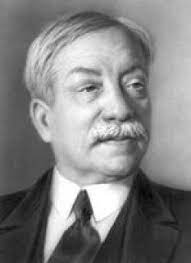
\includegraphics[width=0.65\textwidth]{Galerkin}
	\caption[]{Boris Galerkin (Russia, 1871-1945).}
	\labfig{galerkinphoto}
\end{marginfigure}

\bigskip

\emph{Assuming that problem given by \refeq{absVPag} is well posed, 
the logical question that emerges is if the new problem
given in \refeq{absVPdisc}, is also well posed ...}

\bigskip
The answer is yes, because the discrete problem inherits the properties
of the continuous one. First, observe that:
\begin{itemize}
\item Being $V$ Hilbert, a finite dimensional subspace $V_h \subset V$ is
also Hilbert\sidenote{A finite dimensional subspace is necessarily closed.};\\
\item Since $a$ is bounded in $V$
(i.e., $|a(u,v)| \le N_a\,\lVert u \rVert_V \,\lVert v \rVert_V$ $\forall u,v \in V$),
it is in particular bounded in $V_h$;\\
\item Since $a$ is strongly coercive
(i.e., $a(u,u) \ge \alpha\,\lVert u \rVert_V^2~\forall u \in V$) it is in particular
coercive in $V_h$;\\
\item For the same reason, $\ell(v)$ is also continuous in $V_h$;\\
\end{itemize}
As a corollary of \refthm{RieszVP} in case $a(\cdot,\cdot)$ is symmetric
or \refthm{laxmilgram}, if it is not necessarily symmetric, we have the:
\begin{corollary}
There exists a unique $u_h \in V_h$
that satisfies the problem (\textbf{VF}$_h$): Find $u_h \in V_h$ such that
\begin{equation}
\left.
\begin{array}{rll}
a(u_h,v_h) & = & \ell(v_h)  ~~~\forall v_h \in V_h \\
\end{array}
\right. \nonumber
\end{equation}
\end{corollary}

\bigskip

\emph{The next question is if $u_h$ is computable ...}

\bigskip
The interesting thing about the Galerkin method is that it provides
the \textbf{methodology} to compute $u_h$. If we choose a basis
$\{\phi_1,\phi_2,\dots,\phi_n\}$ of $V_h$, replace the
\refeq{ansatzuh} and take $v_h = \phi_i$ in \refeq{absVPdisc},
we obtain
\begin{equation}
a\left (\sum_{j=1}^{n}{U_j\phi_j}, \phi_i\right) = \sum_{j=1}^{n}{\underbrace{a(\phi_j,\phi_i)}_{A_{ij}}U_j} =
\underbrace{\ell(\phi_i)}_{b_i},~~~i=1,\dots,n
\end{equation}
which is clearly a linear system of equations
\begin{equation}
\mathsf{A} \, \mathbf{U} = \mathsf{b}
\end{equation}
where $\mathbf{U} \in \mathbb{R}^{n}$.
$\mathsf{A} \in \mathbb{R}^{n \times n}$ and $\mathsf{b} \in \mathbb{R}^{n}$
are defined by
\begin{equation}
A_{ij} = a(\phi_j,\phi_i),~~~b_i = \ell(\phi_i).
\end{equation}
About matrix $\mathsf{A}$ we can say:
\begin{itemize}
\item if $a(\phi_j,\phi_i) = a(\phi_i,\phi_j)$ (symmetry of $a$),
clearly $\mathsf{A}$ is also symmetric;\\
\item if $a(v_h,v_h) > 0$ (strong coercivity), taking
any arbitrary nonzero $v_h = \sum_{j=1}^{n}{V_j\phi_j}$
(i.e., $\mathbf{V} \ne \mathbf{0}$), we get
\begin{equation}
a\left (\sum_{j=1}^{n}{V_j\phi_j},\sum_{i=1}^{n}{V_i\phi_i} \right) = \sum_{i=1}^{n}\sum_{j=1}^{n}{V_iA_{ij}V_j}
= \mathbf{V}^{\intercal} \mathsf{A} \mathbf{V} > 0,~~\mathbf{V} \ne \mathbf{0}
\end{equation}
thus, $\mathsf{A}$ is positive definite and therefore \textbf{invertible},
so, we can safely solve the system and find the unique $\mathbf{U}$
that defines $u_h$. \\
\end{itemize}

\section{Galerkin orthogonality \& Best approximation} \index{Galerkin orthogonality}

An important property of the Galerkin solution $u_h$ to
(\textbf{VF}$_h$) can be stated.
Begin by saying that 
\begin{eqnarray}
a(u,v_h) = \ell(v_h) & \forall v_h \in V_h \nonumber \\
a(u_h,v_h) = \ell(v_h) & \forall v_h \in V_h \nonumber
\end{eqnarray}
so, substracting
\begin{eqnarray}
a(u - u_h,v_h) = 0 & \forall v_h \in V_h \nonumber
\end{eqnarray}
This fact, allows us to show the following important lemma:
\begin{lemma}
\lablemma{jcea}
(\textbf{J. C\'ea})
Let $a(\cdot,\cdot)$ and $\ell(\cdot)$ be continuous forms in $V$,
with $a(\cdot,\cdot)$ strongly coercive, then
\begin{equation}
\lVert u - u_h \rVert_V \le \frac{N_a}{\alpha} \lVert u - v_h \rVert_V~~\forall v_h \in V_h
\end{equation}
\end{lemma}
This can be shown by using the trick:
\begin{eqnarray}
a(u-u_h, u-u_h) & = & a(u-u_h, u-u_h+v_h-v_h) =  \nonumber \\
& = &\underbrace{a(u-u_h,v_h-u_h)}_{=0}~+~a(u-u_h,u-v_h) \nonumber \\
& = & a(u-u_h,u-v_h)~~\forall v_h \in V_h \nonumber
\end{eqnarray}
but, by the coercivity $a(u-u_h, u-u_h) \ge \alpha \lVert u-u_h \rVert_V^2$,
then
\begin{equation}
\lVert u - u_h \rVert_V^2 \le \frac{1}{\alpha}a(u-u_h, u-u_h) = \frac{1}{\alpha}a(u-u_h, u-v_h) ~~\forall v_h \in V_h
\end{equation}
and by the continuity $a(u-u_h, u-v_h) \le N_a \lVert u-u_h \rVert_V\lVert u-v_h \rVert_V$,
implying that
\begin{equation}
\lVert u - u_h \rVert_V^2 \le \frac{N_a}{\alpha} \lVert u-u_h \rVert_V\lVert u-v_h \rVert_V ~~\forall v_h \in V_h.
\end{equation}

This is equivalent to say that\sidenote{Note that we may run into trouble if
$\frac{N_a}{\alpha} \gg 1$, because this does not provide a practical
control on the error. Saying that $\lVert u - u_h \rVert_V$ is lower than
a very large number is not that useful.}:
\begin{equation}
\lVert u - u_h \rVert_V \le \frac{N_a}{\alpha} \min_{v_h \in V_h} \lVert u-v_h \rVert_V.
\end{equation}

So far, it has not been assumed that $a(\cdot, \cdot)$ is symmetric.
If $a$ happens to be, so it defines an inner product over $V$, then:

\begin{itemize}
\item $a(u - u_h,v_h) = 0~\forall~v_h \in V_h$ implies that the error $e_h = u-u_h$ is orthogonal to $V_h$,
therefore, we say that the Galerkin approximation $u_h$ is the \textbf{orthogonal projection}
of $u$ onto $V_h$ (see \reffig{orthoproj});\\

\item The Galerkin approximation $u_h$ is \textbf{optimal} in the energy norm, i.e.,
\begin{equation}
\lVert u - u_h \rVert_a \le \lVert u-v_h \rVert_a ~~\forall v_h \in V_h.
\end{equation}
since in this norm the coercivity and continuity constants are both equal to $1$.

\begin{marginfigure}[-4.0cm]
	\includegraphics[width=1.1\textwidth]{orth_proj}
	\caption[]{Classical picture of orthogonal projection in Euclidean spaces.}
	\labfig{orthoproj}
\end{marginfigure}

\end{itemize}

\section{Distance to $V_h$}

Let us briefly comment on an altenative way of thinking these issues.
First, recall that given an inner product, we have a natural way
of defining a \textbf{distance} $d(\cdot, \cdot)$ between two functions
in the space $V$, i.e.,
\begin{equation}
 d(f,g) = \lVert f - g \rVert_V = \sqrt{(f-g,f-g)_V}\nonumber
\end{equation}
This can be the $L^2(\Omega)$ or the $H^1(\Omega)$-inner products.
It can be shown that there exists one and only one element $u_h \in V_h$ such that 
\begin{equation}    
 d(u,u_h) \le d(u,v_h)~~ \forall v_h \in V_h \labeq{d_le_d}
\end{equation}
and $u_h$ is the orthogonal projection of $u$ onto $V_h$.
To construct such $u_h$, let us suppose that a $u_h$ that satisfies \refeq{d_le_d} exists.
Then, given any $v_h \in V_h$ the functional
\begin{equation}
 j(s) = d(u,u_h + s\,v_h)^2 = \left \| u - (u_h + s\,v_h ) \right \|_V^2~~
\end{equation}
will have a minimum at $s = 0$, i.e., 
if $u_h$ minimizes $d(u,u_h)^2$, then $j(0) \le j(s)~\forall s \in \mathbb{R}$. 
Using the linearity and symmetry of the inner product we show that
\begin{eqnarray}
 j(s) = d(u,u_h + s\,v_h)^2 & = &  \left ( u - (u_h + s\,v_h), u - (u_h + s\,v_h) \right )_V = \nonumber \\ 
 & =& (u - u_h, u- u_h)_V  - 2 \, s \, (u-u_h,v_h)_V + s^2 \, (v_h,v_h)_V \nonumber \\
 & = & \lVert u -u_h \rVert^2_V - 2 \, s \, (u-u_h,v_h)_V +  s^2 \, \lVert v_h \rVert^2_V  \nonumber
 \end{eqnarray}
Now, to have a minimum of this functional for all $v_h \in V_h$ 
when $s = 0$, its derivative with respect to $s$ is 
necessarily equal to zero at $s=0$, i.e.,
\begin{eqnarray}
 \frac{dj}{ds}(s=0) = - 2 \, (u-u_h,v_h)_V = 0 ~~\forall~v_h \in V_h \nonumber
\end{eqnarray}
which, again, means that the difference between $u$ and $u_h$ is orthogonal
to all $v_h \in V_h$ and $u_h$ satisfies\sidenote{Notice that this is a variational problem
in which the bilinear form $a(\cdot,\cdot)$
and the linear form $\ell(\cdot)$ are given by the inner product:
\begin{equation}
 \begin{cases}
  a(u_h,v_h) = (u_h, v_h)_V \\
  \nonumber\\
  \ell(v_h) = (u,v_h)_V \\
 \end{cases} \nonumber 
\end{equation}
}
\begin{eqnarray}
  (u_h,v_h)_V = (u,v_h)_V  ~~\forall v_h \in V_h\nonumber
\end{eqnarray}

\section{Conclusion - Consequence of C\'ea's lemma}

The distance from $u$ to $V_h$ estimates de error, so the
idea is that if we build a sequence of discrete function
spaces $\{V_{h,n}\}$ (as is done in the FEM)
with $h\rightarrow 0$ (as $n\rightarrow \infty$),
we pretend that
\begin{equation}
\lim_{h \rightarrow 0} \left ( \min_{v_h \in V_h} \lVert u - v_h \rVert \right ) = 0
\end{equation}
or in simple terms we aim
\begin{equation}
\lim_{h \rightarrow 0} u_h = u
\end{equation}
In the next few chapters we dedicate to study how to construct
discrete function spaces on partitions of $\Omega$ (\textbf{meshes}),
in particular, piecewise polynomial spaces and which are their
approximability and interpolation properties.
Concerning what we have just presented, this is fundamental
because, as we shall see
\begin{equation}
 \min_{v_h \in V_h} \lVert u-v_h \rVert_V \le \lVert u-\mathcal{I}_h{u} \rVert_V ,\nonumber 
\end{equation}
where $\mathcal{I}_h{u}$ stands for the interpolant of the exact
solution $u$ onto the space $V_h$.

So, the plan for the next part is to introduce:

\begin{itemize}
\item[$\circ$] Polynomial spaces on finite element partitions of $\Omega$;
\item[$\circ$] Interpolation operators;
\item[$\circ$] Local estimates of the interpolation error;
\item[$\circ$] Global error estimates;
\item[$\circ$] Some issues about regularity of meshes;
\end{itemize}

\bigskip

... but, before that, to fix some of the ideas of this chapter
we must:

%------------------------------------------------------
\begin{kaobox}[frametitle=Solve the following exercices]
\begin{itemize}

\item (\textbf{Linear Algebra}) Show that of if $\mathsf{A} \in \mathbb{R}^{n\times n}$ is
positive definite ($\mathbf{V}^{\intercal} \mathsf{A} \mathbf{V} > 0~\forall V \in \mathbb{R}^n$),
then, $\mathsf{A}$ is invertible.\\

\item In the optimallity of the Galerkin approximation $u_h$, it is
used that in the energy norm $\lVert \cdot \rVert_a$,
the coercivity and continuity constants are both equal to $1$. Explain. \\

\end{itemize}
\end{kaobox}

\section{{\color{gray!50!yellow} Assignment 4: Projection of functions}}

\begin{kaobox}
Consider the variational problem (orthogonal projection):
Find $u_h \in V_h$ such that
\begin{eqnarray}
  a(u_h,v_h) = \ell(v_h)  ~~\forall v_h \in V_h \nonumber
\end{eqnarray}
where
$$
a(u_h,v_h) =  (u_h,v_h)_V,~~~~\ell(v_h) = (u,v_h)_V
$$
in which $u$ is a given function and $V$ denotes the $L^2(\Omega)$ inner product, i.e.,
\begin{equation}
(v,w)_{L^2(\Omega)} = \int_{\Omega}{v\,w}\,dx \nonumber
\end{equation}
or the $H^1(\Omega)$-inner product
\begin{equation}
(v,w)_{H^1(\Omega)} = \int_{\Omega}{\left (v\,w + \nabla{v} \cdot \nabla{w}\right )}\,dx \nonumber
\end{equation}
Notice that in this problem no boundary conditions are imposed.

\begin{itemize}

\item Implement a script that solves the projection problem;\\

\item First, consider $\Omega$ to be the unit interval $[0,1]$,
partitioned into \texttt{nels} elements, i.e.

\begin{center}
\begin{minipage}{0.9\textwidth}
    \lstinputlisting[language=Python]{1dmesh.py}
\end{minipage}
\end{center}

and let $u$ be the function given by
$$
u(x) = \sin(2\pi\,x)
$$

\begin{itemize}
\item Take $V_h$ to be a space of piecewise polynomial functions of different degree,
i.e., functions that are polynomials of degree $k$ (constants, linears, quadratics, etc)
on each element and discontinuous between elements\sidenote{These spaces are named
as Discontinuous Galerkin (\texttt{DG} in \texttt{FEniCS})}:
\begin{center}
\begin{minipage}{0.8\textwidth}
    \lstinputlisting[language=Python]{VDG.py}
\end{minipage}
\end{center}
Compute $u_h$, the projection of $u$ onto $V_h$ with the $L^2(\Omega)$ inner product.
Take different number of elements (\texttt{nels = 1, 2, 4, 8, 12, 16, 32})
and \texttt{degree = 0, 1, 2}. \\

\item Repeat the previous item using the $H^1(\Omega)$ inner product,
but now take a space of continuous functions between elements\sidenote{These spaces are named
as Continuous Galerkin (\texttt{CG} or \texttt{Lagrange} in \texttt{FEniCS}).
Details about how all these spaces are actually defined and built are explained in the next chapter.}:
\begin{center}
\begin{minipage}{0.8\textwidth}
    \lstinputlisting[language=Python]{VCG.py}
\end{minipage}
\end{center}
with \texttt{degree = 1, 2, 3}. This is alse referred to as a conforming space.\\

\item Plot the solution by reconstructing the corresponding polynomial on each element.
To that end consider accessing the solution values of $u_h$ from the array:
\begin{center}
\begin{minipage}{0.4\textwidth}
    \lstinputlisting[language=Python]{uharray.py}
\end{minipage}
\end{center}
Interpret the number of components in the array and the values
according to the case being considered (discontinuous or continuous
functions and the degree $k$ of the polynomial on each element of the partition).
Then, use the function \texttt{numpy.polyfit} to build the polynomials
on each element and plot using \texttt{matplotlib} (see the example in \reffig{projsdg0}).
\begin{marginfigure}[-4.0cm]
	\includegraphics[width=1.2\textwidth]{projdg.jpg}
	\caption[]{Example of the $L^2(\Omega)$ orthogonal projection of $u(x) = \sin(2\pi x)$
        onto spaces of piecewise constant functions associated to partitions of
        the unit interval.}
	\labfig{projsdg0}
\end{marginfigure}

\end{itemize}

\item Now, consider a 2D case, the unit square $\Omega = [0,1]^2$ and the function
$$
u(x_1,x_2) = \sin(\pi\,x_1) \, \sin(\pi\,x_2)
$$

Compute the $L^2(\Omega)$ projection onto a space of
piecewise constant (discontinuous) functions and
the $H^1(\Omega)$ projection onto a space of continuous
piecewise linear functions. Visualize in \texttt{Paraview}.\\

\item Prepare a short monograph to report the results;

\end{itemize}

\end{kaobox}



\fi
%\input{chapters/femspaces.tex}
%\input{chapters/interpolation.tex}
%\input{chapters/implementationFEM.tex}
%\input{chapters/ellipticproblems.tex}
%\input{chapters/stokes.tex}
%\input{chapters/parabolic.tex}
%\input{chapters/finalcomments.tex}

%\pagelayout{wide} % No margins
%\addpart{Class Options, Commands and Environments}
%\pagelayout{margin} % Restore margins

%\input{chapters/options.tex}
%\input{chapters/textnotes.tex}
%\input{chapters/figsntabs.tex}
%\input{chapters/references.tex}

%\pagelayout{wide} % No margins
%\addpart{Design and Additional Features}
%\pagelayout{margin} % Restore margins

%\input{chapters/layout.tex}
%\input{chapters/mathematics.tex}

\appendix % From here onwards, chapters are numbered with letters, as is the appendix convention

%\pagelayout{wide} % No margins
%\addpart{Appendix}
%\pagelayout{margin} % Restore margins

%\input{chapters/appendix.tex}

%----------------------------------------------------------------------------------------

\backmatter % Denotes the end of the main document content
\setchapterstyle{plain} % Output plain chapters from this point onwards

%----------------------------------------------------------------------------------------
%	BIBLIOGRAPHY
%----------------------------------------------------------------------------------------

% The bibliography needs to be compiled with biber using your LaTeX editor, or on the command line with 'biber main' from the template directory

\defbibnote{bibnote}{Here are the references in citation order.\par\bigskip} % Prepend this text to the bibliography
\printbibliography[heading=bibintoc, title=Bibliography, prenote=bibnote] % Add the bibliography heading to the ToC, set the title of the bibliography and output the bibliography note

%----------------------------------------------------------------------------------------
%	NOMENCLATURE
%----------------------------------------------------------------------------------------

% The nomenclature needs to be compiled on the command line with 'makeindex main.nlo -s nomencl.ist -o main.nls' from the template directory

\nomenclature{$c$}{Speed of light in a vacuum inertial frame}
\nomenclature{$h$}{Planck constant}

\renewcommand{\nomname}{Notation} % Rename the default 'Nomenclature'
\renewcommand{\nompreamble}{The next list describes several symbols that will be later used within the body of the document.} % Prepend this text to the nomenclature

%\printnomenclature % Output the nomenclature


%----------------------------------------------------------------------------------------
%	GLOSSARY
%----------------------------------------------------------------------------------------

% The glossary needs to be compiled on the command line with 'makeglossaries main' from the template directory

\setglossarystyle{listgroup} % Set the style of the glossary (see https://en.wikibooks.org/wiki/LaTeX/Glossary for a reference)
\printglossary[title=Special Terms, toctitle=List of Terms] % Output the glossary, 'title' is the chapter heading for the glossary, toctitle is the table of contents heading

%----------------------------------------------------------------------------------------
%	INDEX
%----------------------------------------------------------------------------------------

% The index needs to be compiled on the command line with 'makeindex main' from the template directory

\printindex % Output the index

%----------------------------------------------------------------------------------------
%	BACK COVER
%----------------------------------------------------------------------------------------

% If you have a PDF/image file that you want to use as a back cover, uncomment the following lines

%\clearpage
%\thispagestyle{empty}
%\null%
%\clearpage
%\includepdf{cover-back.pdf}

%----------------------------------------------------------------------------------------

\end{document}
